\newpage
\chapter{HASIL DAN PEMBAHASAN} \label{BabIV}

Bab ini menyajikan hasil dan analisis dari seluruh tahapan penelitian, mulai dari pengumpulan data, pra-pemrosesan, pembagian dataset, konfigurasi eksperimen, hingga evaluasi performa model VideoMAE dalam mengklasifikasikan gerakan visual Bahasa Isyarat SIBI.\par

%===========================================================================
\section{Pengumpulan Data} \label{IV.Pengumpulan}
%===========================================================================

Dataset yang digunakan dalam penelitian ini diperoleh melalui proses perekaman langsung di Sekolah Luar Biasa Negeri (SLBN) PKK Provinsi Lampung, sebagaimana telah dijelaskan pada Subbab~\ref{III.Pengumpulan_Data}. Dataset mencakup 10 kelas kata dasar Bahasa Isyarat SIBI yang umum digunakan dalam lingkungan sekolah, yaitu \textit{aku}, \textit{bapak}, \textit{bawa}, \textit{guru}, \textit{ibu}, \textit{kamu}, \textit{mau}, \textit{pulang}, \textit{sekolah}, dan \textit{suka}. Setiap isyarat direkam oleh beberapa responden (peserta didik yang fasih menggunakan SIBI) dan ada beberapa data yang berasal dari luar siswa SLBN PKK Lampung dalam ruangan tertutup dengan pencahayaan stabil dan latar belakang polos menggunakan kamera iPhone 11 beresolusi 1080p pada 30 fps.\par

Total dataset yang berhasil dikumpulkan adalah 924 klip video dalam format MP4. Distribusi jumlah klip per kelas disajikan pada Tabel~\ref{tab:4.distribusi_kelas}.\par

\begin{table}[H]
\centering
\caption{Distribusi jumlah klip video per kelas dataset SIBI}
\label{tab:4.distribusi_kelas}
{\setlength{\tabcolsep}{3pt}
\footnotesize
\begin{tabular}{|r|l|r||r|l|r|}
\hline
\rowcolor{gray!15} \multicolumn{1}{|c|}{No} & \multicolumn{1}{c|}{Kelas} & \multicolumn{1}{c|}{Jumlah Klip} & \multicolumn{1}{c|}{No} & \multicolumn{1}{c|}{Kelas} & \multicolumn{1}{c|}{Jumlah Klip} \\
\hline
1  & Aku     & 90  & 6  & Kamu    & 93 \\
\hline
2  & Bapak   & 90  & 7  & Mau     & 99 \\
\hline
3  & Bawa    & 88  & 8  & Pulang  & 99 \\
\hline
4  & Guru    & 90  & 9  & Sekolah & 89 \\
\hline
5  & Ibu     & 96  & 10 & Suka    & 90 \\
\hline
\multicolumn{5}{|c|}{Total} & 924 \\
\hline
\end{tabular}
}
\end{table}

Distribusi antarkelas pada Tabel~\ref{tab:4.distribusi_kelas} menunjukkan jumlah sampel yang relatif seimbang, dengan rentang antara 88 klip (kelas \textit{Bawa}) hingga 99 klip (kelas \textit{Mau} dan \textit{Pulang}). Contoh frame representatif dari setiap kelas setelah proses pemburaman wajah dapat dilihat pada Lampiran~\ref{app:contoh_frame}. Keseimbangan ini penting untuk memastikan model tidak mengalami bias terhadap kelas tertentu selama pelatihan.\par

%===========================================================================
\section{Prapemrosesan Data} \label{IV.Praproses}
%===========================================================================

Seluruh klip video mentah yang telah dikumpulkan melalui tahap prapemrosesan untuk menghasilkan format masukan yang sesuai dengan arsitektur VideoMAE, mengikuti prosedur yang telah dirancang pada Subbab~\ref{III.Data_Preprocessing}. Keluaran dari tahap ini adalah tensor berukuran $(3, 16, 224, 224)$ per klip, yang merepresentasikan 3 kanal warna, 16 frame temporal, dan resolusi spasial $224\times224$ piksel.\par

Tahapan prapemrosesan yang diterapkan adalah sebagai berikut:
\begin{enumerate}[noitemsep]
  \item Standardisasi resolusi: Setiap frame dalam klip di-\textit{resize} ke dimensi $224\times224$ piksel untuk memenuhi ukuran masukan standar ViT dan VideoMAE.
  \item Standardisasi laju cuplik: Seluruh video disamakan ke 30 FPS agar panjang temporal gestur terwakili secara konsisten antar klip.
  \item \textit{Sampling} frame: Sebanyak 16 frame diambil dari setiap klip menggunakan strategi \textit{uniform sampling} (default) atau \textit{dense sampling} sesuai konfigurasi eksperimen.
  \item Normalisasi piksel: Nilai piksel dinormalisasi menggunakan rata-rata dan standar deviasi ImageNet ($\boldsymbol{\mu}=(0.485,\;0.456,\;0.406)$, $\boldsymbol{\sigma}=(0.229,\;0.224,\;0.225)$) agar distribusi nilai masukan stabil untuk proses optimasi.
  \item Augmentasi data: Diterapkan augmentasi berupa \textit{horizontal inversion}, \textit{brightness adjustment}, dan \textit{downsampling} frame pada data latih untuk memperkaya variasi sampel.
\end{enumerate}

Metadata setiap klip beserta label kelas dan informasi fold disimpan dalam berkas CSV sebagai referensi tunggal yang dimuat oleh \textit{DataLoader} selama pelatihan, sehingga seluruh eksperimen dapat direproduksi secara konsisten.\par

%===========================================================================
\subsection{Standardisasi Video} \label{IV.Standardisasi}
%===========================================================================

Standardisasi video merupakan langkah pertama dalam tahap pra-pemrosesan yang bertujuan menyeragamkan resolusi, laju cuplik, dan format seluruh klip dalam dataset agar memenuhi persyaratan masukan model VideoMAE. Setiap klip diubah resolusinya menjadi $224\times224$ piksel, laju cupliknya diseragamkan menjadi 30 FPS, dan kanal audio dihapus. Proses ini dikerjakan menggunakan FFmpeg melalui antarmuka \texttt{subprocess} Python sehingga dapat dijalankan secara otomatis untuk seluruh video dalam dataset. Fungsi \texttt{process\_video()} pada Kode~\ref{lst:standardisasi} menangani standardisasi sekaligus menerima filter augmentasi opsional melalui parameter \texttt{extra\_filter}.\par

\begin{lstlisting}[caption={Kode standardisasi video menggunakan FFmpeg}, label={lst:standardisasi}]
def process_video(input_path: Path, output_path: Path,
                  size: int = 224, fps: int = 30,
                  extra_filter: str = None):
    if output_path.exists():
        return True  # Lewati jika sudah diproses

    output_path.parent.mkdir(parents=True, exist_ok=True)

    vf_str = f"scale={size}:{size},fps={fps}"
    if extra_filter:
        vf_str += f",{extra_filter}"

    cmd = [
        "ffmpeg", "-y", "-threads", "0",
        "-i", str(input_path),
        "-vf", vf_str,
        "-c:v", "libx264", "-preset", "fast",
        "-crf", "23", "-an",
        str(output_path)
    ]
    subprocess.run(cmd,
                   stdout=subprocess.DEVNULL,
                   stderr=subprocess.DEVNULL,
                   check=True)
\end{lstlisting}

Fungsi \texttt{process\_video()} menerima \texttt{input\_path} sebagai sumber video asli, \texttt{output\_path} sebagai tujuan penyimpanan, dan \texttt{extra\_filter} sebagai filter FFmpeg opsional untuk keperluan augmentasi. Parameter \texttt{-threads 0} memungkinkan FFmpeg memanfaatkan seluruh \textit{core} CPU yang tersedia secara otomatis sehingga proses standardisasi berjalan lebih efisien. Parameter \texttt{-crf 23} dengan kodek \texttt{libx264} menjamin kualitas visual yang baik dengan ukuran berkas yang terkendali. Pemeriksaan \texttt{output\_path.exists()} di baris~4--5 memungkinkan proses dilanjutkan dari titik terakhir tanpa mengulang video yang sudah diproses sebelumnya.\par

%===========================================================================
\subsection{Augmentasi Data} \label{IV.Augmentasi}
%===========================================================================

Augmentasi data dilakukan untuk memperkaya variasi sampel pelatihan dan meningkatkan kemampuan generalisasi model terhadap kondisi visual yang beragam. Berbeda dengan augmentasi pada data gambar statis, augmentasi video diterapkan menggunakan filter FFmpeg agar perubahan bersifat konsisten di seluruh \textit{frame} dalam satu klip. Pada penelitian ini diterapkan tiga jenis augmentasi: (1) \textit{inversi warna} (\texttt{negate}) untuk mengubah representasi warna video menjadi nilai komplemen, (2) \textit{penguatan kecerahan piksel} sebesar $1.2\times$ menggunakan filter \texttt{lutrgb}, dan (3) \textit{simulasi resolusi rendah} dengan \textit{downsampling} ke setengah resolusi kemudian dikembalikan ke ukuran semula menggunakan interpolasi \textit{nearest-neighbor}. Setiap klip asli menghasilkan tiga klip augmentasi sehingga jumlah data pelatihan meningkat hingga empat kali lipat. Kode~\ref{lst:augmentasi} menunjukkan implementasi pembuatan seluruh varian augmentasi untuk setiap klip.\par

\begin{lstlisting}[caption={Kode augmentasi data video}, label={lst:augmentasi}]
# A. Standardisasi (versi asli)
process_video(src_path, path_orig, size=args.size)

# B. Augmentasi 1: Inversi warna
process_video(src_path, path_inv,
              size=args.size,
              extra_filter="negate")

# C. Augmentasi 2: Penguatan kecerahan piksel (x1.2)
process_video(src_path, path_mult,
              size=args.size,
              extra_filter="lutrgb=r=val*1.2:g=val*1.2:b=val*1.2")

# D. Augmentasi 3: Simulasi resolusi rendah
down_size = args.size // 2
process_video(src_path, path_down,
              size=args.size,
              extra_filter=(
                  f"scale={down_size}:{down_size},"
                  f"scale={args.size}:{args.size}:flags=neighbor"
              ))
\end{lstlisting}

Gambar~\ref{fig:aug_contoh} menampilkan contoh satu \textit{frame} dari keempat varian klip untuk kata ``Aku'' (video ke-90). Terlihat bahwa inversi warna menghasilkan tampilan komplementer yang kontras, penguatan kecerahan meningkatkan intensitas piksel secara merata, sedangkan simulasi resolusi rendah menghasilkan tekstur yang lebih kasar akibat interpolasi \textit{nearest-neighbor}.\par

\begin{figure}[H]
  \centering
  \fbox{\begin{minipage}{0.97\linewidth}
\centering
\fbox{\begin{minipage}{0.97\linewidth}
\centering
\fbox{\begin{minipage}{0.97\linewidth}
\centering
\fbox{\begin{minipage}{0.97\linewidth}
\centering
\begin{subfigure}[b]{0.22\textwidth}
    \centering
    
\includegraphics[width=\textwidth]{figure/aug_orig.jpg}
    \caption{Asli}
    \label{fig:aug_orig}
  \end{subfigure}
\end{minipage}}
\end{minipage}}
\end{minipage}}
\end{minipage}}
\hfill
  \begin{subfigure}[b]{0.22\textwidth}
    \centering
    
\includegraphics[width=\textwidth]{figure/aug_inv.jpg}
    \caption{Inversi warna}
    \label{fig:aug_inv}
  \end{subfigure}
  \hfill
  \begin{subfigure}[b]{0.22\textwidth}
    \centering
    
\includegraphics[width=\textwidth]{figure/aug_mult.jpg}
    \caption{Penguatan kecerahan}
    \label{fig:aug_mult}
  \end{subfigure}
  \hfill
  \begin{subfigure}[b]{0.22\textwidth}
    \centering
    
\includegraphics[width=\textwidth]{figure/aug_down.jpg}
    \caption{Resolusi rendah}
    \label{fig:aug_down}
  \end{subfigure}
  \caption{Contoh \textit{frame} hasil augmentasi pada klip ``Aku'' (video ke-90, \textit{frame} ke-39)}
  \label{fig:aug_contoh}
\end{figure}

Augmentasi hanya diterapkan pada data pelatihan di setiap \textit{fold}, sedangkan data validasi tetap menggunakan klip versi asli agar evaluasi merepresentasikan kondisi data dunia nyata. Pendekatan ini mengikuti prinsip bahwa augmentasi berfungsi sebagai regularisasi implisit selama pelatihan, bukan sebagai cara meningkatkan skor evaluasi secara artifisial.\par

%===========================================================================
\section{Pembagian Dataset} \label{IV.Pembagian}
%===========================================================================

Dataset yang terdiri dari 924 klip video dibagi menggunakan skema \textit{Stratified 5-Fold Cross Validation} ($k=5$), sebagaimana yang dirancang pada Subbab~\ref{III.Data_Preprocessing}. Skema stratifikasi memastikan proporsi setiap kelas tetap seimbang pada subset latih maupun validasi di setiap fold, sehingga tidak ada distorsi distribusi kelas akibat pembagian acak.\par

Pada setiap fold, sekitar 80\% dari total data digunakan sebagai data latih ($\approx739$ klip) dan sekitar 20\% sebagai data validasi ($\approx185$ klip). Setiap klip memperoleh kesempatan menjadi data validasi tepat satu kali sepanjang kelima iterasi, sehingga estimasi performa lebih stabil dan representatif. Tabel~\ref{tab:4.fold_split} merangkum pembagian data pada masing-masing fold.\par

\begin{table}[H]
\centering
\caption{Pembagian data per fold pada skema \textit{Stratified 5-Fold Cross Validation}}
\label{tab:4.fold_split}
{\setlength{\tabcolsep}{3pt}
\footnotesize
\begin{tabular}{|r|r|r|}
\hline
\rowcolor{gray!15} \multicolumn{1}{|c|}{Fold} & \multicolumn{1}{c|}{Data Latih} & \multicolumn{1}{c|}{Data Validasi} \\
\hline
1 & 739 & 185 \\
\hline
2 & 739 & 185 \\
\hline
3 & 739 & 185 \\
\hline
4 & 739 & 185 \\
\hline
5 & 740 & 184 \\
\hline
Total & \multicolumn{2}{r|}{924} \\
\hline
\end{tabular}
}
\end{table}

Pembagian fold dilaksanakan menggunakan \texttt{StratifiedKFold} dari \textit{library} scikit-learn dengan pendekatan \textit{split-first}, yaitu pembagian dilakukan terlebih dahulu pada klip asli sebelum augmentasi diterapkan. Pendekatan ini mencegah kebocoran data (\textit{data leakage}), yang memungkinkan klip asli dan versi augmentasinya masuk ke \textit{fold} yang berbeda sehingga model secara tidak langsung ``melihat'' data validasi selama pelatihan. Kode~\ref{lst:kfold} menunjukkan implementasi pembagian dataset.\par

\begin{lstlisting}[caption={Kode pembagian dataset dengan \textit{Stratified K-Fold}}, label={lst:kfold}]
X_dummy  = np.zeros(len(original_data))
y_labels = np.array([item[1] for item in original_data])

skf = StratifiedKFold(
    n_splits=args.num_folds,
    shuffle=True,
    random_state=args.seed
)
folds_indices = list(skf.split(X_dummy, y_labels))
\end{lstlisting}

Parameter \texttt{shuffle=True} memastikan data diacak sebelum pembagian \textit{fold} dilakukan, sedangkan \texttt{random\_state=42} menjamin bahwa setiap percobaan yang diulang menghasilkan pembagian yang identik (\textit{reproducible}). \texttt{StratifiedKFold} menjaga proporsi setiap kelas pada masing-masing \textit{fold} sesuai distribusi dataset keseluruhan, sehingga evaluasi antarfold dapat dibandingkan secara adil.\par

Setelah pembagian \textit{fold} ditetapkan dan seluruh video selesai diproses, dibuat berkas CSV untuk setiap \textit{fold} yang berfungsi sebagai manifes dataset yang dibaca oleh \textit{data loader} VideoMAE. Format yang digunakan adalah \textit{path} relatif video diikuti label numerik kelas, dipisahkan oleh spasi. Pada data pelatihan, klip asli dan ketiga varian augmentasinya dimasukkan sekaligus, sedangkan data validasi hanya memuat klip versi asli. Kode~\ref{lst:writecsv} menunjukkan implementasi pembuatan CSV berdasarkan indeks \textit{fold}.\par

\begin{lstlisting}[caption={Kode penulisan berkas CSV untuk setiap \textit{fold}}, label={lst:writecsv}]
for fold_idx, (train_idx, val_idx) in enumerate(folds_indices):
    fold_id       = fold_idx + 1
    train_records = []
    val_records   = []

    # Data pelatihan: klip asli + seluruh augmentasi
    for idx in train_idx:
        src_path = original_data[idx][0]
        if src_path in processed_map:
            data = processed_map[src_path]
            train_records.append(
                VideoRecord(data['orig'], data['label']))
            for aug_path in data['aug']:
                train_records.append(
                    VideoRecord(aug_path, data['label']))

    # Data validasi: hanya klip asli
    for idx in val_idx:
        src_path = original_data[idx][0]
        if src_path in processed_map:
            data = processed_map[src_path]
            val_records.append(
                VideoRecord(data['orig'], data['label']))

    write_csv(train_records,
              output_dir / f"train_fold_{fold_id}.csv",
              base_dir=output_dir)
    write_csv(val_records,
              output_dir / f"val_fold_{fold_id}.csv",
              base_dir=output_dir)
\end{lstlisting}

Setiap pasangan berkas \texttt{train\_fold\_N.csv} dan \texttt{val\_fold\_N.csv} yang dihasilkan menjadi masukan langsung bagi skrip pelatihan VideoMAE. Selain CSV, \texttt{label\_map.json} juga disimpan untuk merekam pemetaan antara nama kelas SIBI dan indeks numerik, sehingga hasil prediksi model dapat diinterpretasikan kembali ke nama kelas asli.\par

%===========================================================================
\section{Konfigurasi Eksperimen} \label{IV.Konfigurasi}
%===========================================================================

Seluruh eksperimen pelatihan dijalankan pada platform komputasi awan RunPod menggunakan GPU NVIDIA GeForce RTX 4090 (24 GB VRAM) dengan PyTorch 2.8 pada Python 3.10. Pengukuran waktu inferensi dilakukan secara terpisah pada laptop lokal dengan GPU NVIDIA GeForce RTX 3050 Laptop (4 GB VRAM). Konfigurasi umum yang berlaku pada semua eksperimen kecuali disebutkan lain dirangkum pada Tabel~\ref{tab:4.umum_config}.\par

\begin{table}[H]
\centering
\caption{Konfigurasi umum yang berlaku pada seluruh eksperimen}
\label{tab:4.umum_config}
{\setlength{\tabcolsep}{3pt}
\footnotesize
\begin{tabular}{|l|l|}
\hline
\rowcolor{gray!15} \multicolumn{1}{|c|}{\textbf{Parameter}} & \multicolumn{1}{c|}{\textbf{Nilai}} \\
\hline
Jumlah kelas              & 10 \\
\hline
Resolusi masukan          & $224\times224$ piksel \\
\hline
Jumlah frame per klip     & 16 \\
\hline
\textit{Optimizer}        & AdamW \\
\hline
\textit{Loss function}    & \textit{Cross Entropy} \\
\hline
Skema validasi            & \textit{Stratified 5-Fold Cross Validation} \\
\hline
\textit{Early stopping}   & Aktif \\
\hline
\end{tabular}
}
\end{table}

Secara keseluruhan terdapat 12 eksperimen utama VideoMAE (E1--E12) serta dua model pembanding (ViViT dan I3D) yang dirancang secara bertahap untuk menjawab pertanyaan penelitian. Gambaran umum rancangan seluruh eksperimen telah disajikan pada Tabel~\ref{tab:3.rancangan_eksperimen} di Bab~\ref{BabIII}.\par

%===========================================================================
\subsection{Implementasi Pelatihan Dua Tahap VideoMAE} \label{IV.ImplTwostage}
%===========================================================================

Pelatihan model VideoMAE menggunakan strategi dua tahap (\textit{two-stage fine-tuning}) yang lebih stabil dibandingkan \textit{fine-tuning} langsung secara penuh pada dataset berukuran sedang. Pada \textit{Stage}~1, seluruh \textit{backbone} (encoder ViT) dibekukan dan hanya \textit{classification head} yang dilatih dengan \textit{learning rate} tinggi ($10^{-3}$) tanpa \textit{warmup}. Tujuannya adalah menginisialisasi \textit{head} agar berada pada ruang representasi yang sesuai sebelum seluruh jaringan dibuka. Pada \textit{Stage}~2, seluruh lapisan model dibuka dan \textit{fine-tuning} dilakukan secara \textit{end-to-end} dengan \textit{learning rate} yang jauh lebih kecil ($10^{-5}$) disertai \textit{warmup} 5 \textit{epoch} untuk mencegah kerusakan bobot \textit{pretrained} pada awal pelatihan.\par

Seluruh parameter konfigurasi dirangkum dalam \textit{dataclass} \texttt{TwoStageConfig} sehingga variasi eksperimen dapat dilakukan tanpa mengubah logika inti pelatihan. Kode~\ref{lst:twostageconfig} menunjukkan struktur konfigurasi tersebut.\par

\begin{lstlisting}[caption={Kode konfigurasi pelatihan dua tahap VideoMAE}, label={lst:twostageconfig}]
@dataclass
class TwoStageConfig:
    label:           str           = "ViT-Small | SSV2 | Two-Stage"
    output_base:     Path          = PROJECT_ROOT / "work_dirs"
    model_name:      str           = "vit_small_patch16_224"
    pretrained_file: Optional[str] = \
                     "videomae_small_patch16_224_ssv2.pth"

    num_folds:     int   = 5
    num_frames:    int   = 16
    sampling_rate: int   = 1
    batch_size:    int   = 12
    num_workers:   int   = 12
    grad_accum:    int   = 2      # effective batch = 12 x 2 = 24
    weight_decay:  float = 0.05
    early_stop_patience: Optional[int] = 5

    # Stage 1 -- head only
    stage1_epochs:    int  = 5
    stage1_lr:        str  = "1e-3"
    stage1_warmup:    int  = 0
    stage1_mixup_off: bool = True  # label murni untuk head baru

    # Stage 2 -- full fine-tune
    stage2_epochs:    int  = 50
    stage2_lr:        str  = "1e-5"
    stage2_warmup:    int  = 5
    stage2_clip_grad: str  = "1.0"
    stage2_mixup_off: bool = False
\end{lstlisting}

Penggunaan \textit{dataclass} memungkinkan pembuatan varian konfigurasi melalui \texttt{dataclasses.replace()} tanpa menduplikasi kode. Atribut \texttt{grad\_accum} mengimplementasikan \textit{gradient accumulation}, yaitu teknik untuk mensimulasikan \textit{batch size} yang lebih besar ($12 \times 2 = 24$) pada GPU dengan memori terbatas. \textit{Mixup} dinonaktifkan pada \textit{Stage}~1 (\texttt{stage1\_mixup\_off = True}) agar \textit{head} mempelajari label asli secara langsung sebelum \textit{fine-tuning} penuh pada \textit{Stage}~2.\par

Setiap \textit{stage} pelatihan VideoMAE dijalankan melalui skrip \texttt{run\_class\_finetuning.py} bawaan VideoMAE yang dipanggil sebagai \textit{subprocess} Python. Fungsi \texttt{build\_stage1\_command()} merakit daftar argumen untuk \textit{Stage}~1 dengan memuat bobot \textit{pretrained} dari SSV2, sebagaimana ditunjukkan pada Kode~\ref{lst:stage1cmd}.\par

\begin{lstlisting}[caption={Kode pembangunan perintah \textit{Stage} 1 VideoMAE}, label={lst:stage1cmd}]
def build_stage1_command(config, num_classes,
                          train_csv, val_csv,
                          fold_output_dir) -> List[str]:
    stage_dir = fold_output_dir / "stage1"
    cmd = _common_finetune_args(
        config, num_classes, train_csv, val_csv, stage_dir)

    pretrained = config.pretrained_path()
    if pretrained is not None:
        cmd += ["--finetune", str(pretrained),
                "--model_key", "module|model"]

    cmd += [
        "--lr",             config.stage1_lr,
        "--epochs",         str(config.stage1_epochs),
        "--save_ckpt_freq", str(config.stage1_epochs),
        "--warmup_epochs",  str(config.stage1_warmup),
        "--clip_grad",      config.stage1_clip_grad,
        "--use_checkpoint",
    ]
    if config.stage1_mixup_off:
        cmd += ["--mixup", "0", "--cutmix", "0", "--reprob", "0"]
    return cmd
\end{lstlisting}

Parameter \texttt{-{}-save\_ckpt\_freq} diset sama dengan jumlah \textit{epoch Stage}~1 agar \textit{checkpoint} hanya disimpan satu kali di akhir pelatihan, menghindari akumulasi berkas \textit{checkpoint} yang memakan ruang penyimpanan. Parameter \texttt{-{}-use\_checkpoint} mengaktifkan \textit{gradient checkpointing} untuk mengurangi penggunaan memori GPU dengan menyimpan hanya sebagian aktivasi dan melakukan komputasi ulang saat dibutuhkan selama \textit{backward pass}.\par

Setelah \textit{Stage}~1 selesai, \textit{checkpoint} terbaiknya digunakan sebagai titik awal \textit{Stage}~2 untuk \textit{fine-tuning} penuh seluruh lapisan model. Kode~\ref{lst:stage2cmd} menunjukkan pembangunan perintah \textit{Stage}~2.\par

\begin{lstlisting}[caption={Kode pembangunan perintah \textit{Stage} 2 VideoMAE}, label={lst:stage2cmd}]
def build_stage2_command(config, num_classes,
                          train_csv, val_csv,
                          fold_output_dir,
                          stage1_checkpoint) -> List[str]:
    stage_dir = fold_output_dir / "stage2"
    cmd = _common_finetune_args(
        config, num_classes, train_csv, val_csv, stage_dir)
    cmd += [
        "--finetune",       str(stage1_checkpoint),
        "--lr",             config.stage2_lr,
        "--epochs",         str(config.stage2_epochs),
        "--save_ckpt_freq", "5",
        "--warmup_epochs",  str(config.stage2_warmup),
        "--clip_grad",      config.stage2_clip_grad,
        "--use_checkpoint",
    ]
    return cmd
\end{lstlisting}

Pada \textit{Stage}~2, argumen \texttt{-{}-finetune} memuat \textit{checkpoint Stage}~1 alih-alih bobot \textit{pretrained} eksternal, sehingga pelatihan dilanjutkan dari representasi yang sudah teradaptasi dengan distribusi data SIBI. \textit{Checkpoint} disimpan setiap 5 \textit{epoch} (\texttt{-{}-save\_ckpt\_freq 5}) untuk menyediakan titik pemulihan apabila proses pelatihan terganggu.\par

%===========================================================================
\subsection{Implementasi \textit{Early Stopping}} \label{IV.EarlyStopping}
%===========================================================================

Mekanisme \textit{early stopping} diimplementasikan pada fungsi \texttt{run\_stage()} yang bertanggung jawab mengeksekusi perintah pelatihan VideoMAE dan memantau perkembangannya secara \textit{real-time}. Fungsi ini membaca keluaran standar proses secara baris per baris: setiap baris berbentuk JSON yang diterbitkan VideoMAE diurai untuk mendapatkan metrik \texttt{val\_acc1} (akurasi validasi Top-1). Apabila akurasi tidak meningkat selama sejumlah \textit{epoch} yang ditentukan oleh \texttt{early\_stop\_patience}, proses dihentikan lebih awal untuk mencegah \textit{overfitting} dan menghemat waktu komputasi. Kode~\ref{lst:earlystop} menunjukkan implementasi inti mekanisme ini.\par

\begin{lstlisting}[caption={Kode eksekusi \textit{subprocess} dan \textit{early stopping}}, label={lst:earlystop}]
process = subprocess.Popen(
    cmd, stdout=subprocess.PIPE,
    stderr=subprocess.STDOUT, text=True,
    cwd=cwd, env=_videomae_env(),
)

best_acc, best_patience_acc, no_improve_count = 0.0, 0.0, 0

for line in process.stdout:
    print(line, end="")
    if not (line.strip().startswith("{")
            and line.strip().endswith("}")):
        continue

    data = json.loads(line.strip())
    if "val_acc1" not in data:
        continue

    acc1 = data["val_acc1"]
    if acc1 > best_acc:
        best_acc = acc1

    if acc1 > best_patience_acc:
        best_patience_acc = acc1
        no_improve_count  = 0
    else:
        no_improve_count += 1

    if (early_stop_patience is not None
            and no_improve_count >= early_stop_patience):
        print(f"[EARLY STOP] val_acc1 tidak membaik "
              f"selama {early_stop_patience} epoch.")
        process.terminate()
        break
\end{lstlisting}

Desain menggunakan dua variabel terpisah untuk melacak akurasi terbaik, yaitu \texttt{best\_acc} dan \texttt{best\_patience\_acc}, merupakan keputusan teknis yang penting. Variabel \texttt{best\_patience\_acc} hanya diperbarui dari baris JSON ringkasan akhir \textit{epoch}, sementara \texttt{best\_acc} juga dapat diperbarui dari baris teks biasa yang muncul lebih awal dalam aliran keluaran. Pemisahan ini mencegah penghitungan \textit{patience} yang salah apabila terdapat baris laporan akurasi pertengahan \textit{epoch} yang nilainya melebihi JSON ringkasan \textit{epoch} sebelumnya, yang dapat menyebabkan \textit{counter early stopping} tidak pernah bertambah meskipun model sebenarnya tidak mengalami peningkatan nyata.\par

%===========================================================================
\section{Hasil Eksperimen} \label{IV.Hasil}
%===========================================================================

Bagian ini menyajikan hasil dan analisis dari seluruh rangkaian eksperimen yang dilakukan untuk mengevaluasi performa model VideoMAE dalam mengklasifikasikan gerakan visual Bahasa Isyarat SIBI. Keseluruhan eksperimen menggunakan skema \textit{5-Fold Cross Validation} sebagaimana telah dirancang pada Bab~\ref{BabIII}, sehingga setiap nilai akurasi yang dilaporkan merupakan rata-rata dari kelima lipatan kecuali disebutkan lain. Terdapat enam kelompok eksperimen yang dianalisis secara berurutan: (1) perbandingan konfigurasi \textit{backbone} dan dataset \textit{pre-train}, (2) perbandingan strategi pelatihan \textit{pre-train} versus \textit{scratch}, (3) perbandingan strategi \textit{sampling} frame, (4) analisis pengaruh jumlah \textit{epoch}, (5) pengaruh augmentasi \textit{mixup}, \textit{CutMix}, dan \textit{reprob} terhadap performa model, serta (6) perbandingan lintas arsitektur antara VideoMAE, ViViT, dan model \textit{baseline} I3D. Setiap kelompok eksperimen diberi kode unik (E1, E2, ...) untuk memudahkan rujukan silang antar pembahasan.\par

%===========================================================================
\subsection{Perbandingan \textit{Backbone} dan Dataset \textit{Pre-train} VideoMAE} \label{IV.Sek1}
%===========================================================================

Pada bagian ini, empat konfigurasi model VideoMAE dibandingkan untuk menentukan kombinasi \textit{backbone} dan dataset \textit{pre-train} yang paling sesuai dalam mengklasifikasikan gerakan visual SIBI. Variasi dilakukan pada dua dimensi: jenis \textit{backbone} (ViT-Small dan ViT-Base) serta dataset yang digunakan untuk \textit{pre-training} (Kinetics-400 dan Something-Something V2). Kinetics-400 merupakan dataset aksi berbasis konteks objek dan latar belakang, sedangkan SSV2 berfokus pada gerakan relatif tangan terhadap objek domain yang secara intuitif lebih dekat dengan karakteristik isyarat tangan pada SIBI. Seluruh model dilatih dengan protokol pelatihan yang identik menggunakan dataset SIBI yang sama. Konfigurasi eksperimen pada bagian ini dirangkum pada Tabel~\ref{tab:4.s1_config}.\par

\begin{table}[H]
\centering
\caption{Konfigurasi eksperimen perbandingan \textit{backbone} dan dataset \textit{pre-train}}
\label{tab:4.s1_config}
{\setlength{\tabcolsep}{3pt}
\footnotesize
\begin{tabular}{|l|l|l|l|l|}
\hline
\rowcolor{gray!15} \multicolumn{1}{|c|}{\textbf{Parameter}} & \multicolumn{1}{c|}{\textbf{E1}} & \multicolumn{1}{c|}{\textbf{E2}} & \multicolumn{1}{c|}{\textbf{E3}} & \multicolumn{1}{c|}{\textbf{E4}} \\
\hline
\textit{Backbone} & ViT-Small & ViT-Base & ViT-Small & ViT-Base \\
\hline
Dataset \textit{Pre-train} & Kinetics-400 & Kinetics-400 & SSV2 & SSV2 \\
\hline
Strategi Pelatihan & \multicolumn{4}{l|}{\textit{Fine-tune} 1-tahap} \\
\hline
\textit{Epoch} & \multicolumn{1}{r|}{50} & \multicolumn{1}{r|}{50} & \multicolumn{1}{r|}{50} & \multicolumn{1}{r|}{50} \\
\hline
\textit{Batch Size} & \multicolumn{1}{r|}{16} & \multicolumn{1}{r|}{16} & \multicolumn{1}{r|}{16} & \multicolumn{1}{r|}{16} \\
\hline
\textit{Learning Rate} & \multicolumn{1}{r|}{$10^{-3}$} & \multicolumn{1}{r|}{$10^{-3}$} & \multicolumn{1}{r|}{$10^{-3}$} & \multicolumn{1}{r|}{$10^{-3}$} \\
\hline
\textit{Hyperparameter} Lain & \multicolumn{4}{l|}{Sama dengan Tabel~\ref{tab:4.umum_config}} \\
\hline
\end{tabular}
}
\end{table}

Tabel~\ref{tab:4.s1_fold} menampilkan nilai \textit{Best Val Acc@1} pada setiap fold untuk keempat konfigurasi eksperimen, sedangkan Tabel~\ref{tab:4.s1_rekap} merangkum rata-rata akurasi fold beserta metrik evaluasi gabungan lainnya.\par

\begin{table}[H]
\centering
\caption{Nilai \textit{Best Val Acc@1} (\%) per fold dan ringkasan hasil eksperimen E1--E4}
\label{tab:4.s1_fold}
{\setlength{\tabcolsep}{3pt}
\footnotesize
\begin{tabular}{|l|r|r|r|r|r|r|r|}
\hline
\rowcolor{gray!15} \multicolumn{1}{|c|}{Kode} & \multicolumn{1}{c|}{Fold 1} & \multicolumn{1}{c|}{Fold 2} & \multicolumn{1}{c|}{Fold 3} & \multicolumn{1}{c|}{Fold 4} & \multicolumn{1}{c|}{Fold 5} & \multicolumn{1}{c|}{\makecell[c]{Rata-\\rata}} & \multicolumn{1}{c|}{Terbaik} \\
\hline
\rowcolor{highlightpink}E1 & 24.32 & 25.54 & 23.78 & 28.65 & 23.24 & 25.11 & 28.65 \\
\hline
E2 & 31.35 & 27.17 & 30.81 & 34.05 & 27.03 & 30.08 & 34.05 \\
\hline
\rowcolor{highlightgreen}E3 & 35.14 & 42.39 & 31.35 & 34.59 & 32.43 & 35.18 & 42.39 \\
\hline
E4 & 38.38 & 32.61 & 24.86 & 34.59 & 35.14 & 33.12 & 38.38 \\
\hline
\end{tabular}
}
\end{table}

\begin{table}[H]
\centering
\caption{Rekapitulasi rata-rata akurasi fold dan metrik evaluasi gabungan: E1--E4}
\label{tab:4.s1_rekap}
{\setlength{\tabcolsep}{3pt}
\footnotesize
\begin{tabular}{|l|l|l|r|r|r|}
\hline
\rowcolor{gray!15} \multicolumn{1}{|c|}{\textbf{Kode}} & \multicolumn{1}{c|}{\textit{\textbf{Backbone}}} & \multicolumn{1}{c|}{\textit{\textbf{Pre-train}}} & \multicolumn{1}{c|}{\makecell[c]{\textbf{Rata-rata}\\\textbf{Acc (\%)}}} & \multicolumn{1}{c|}{\makecell[c]{\textbf{\textit{Macro}}\\\textbf{F1 (\%)}}} & \multicolumn{1}{c|}{\textbf{MAE}} \\
\hline
E1 & ViT-Small & K400 & 25.11 & 16.16 & 2.3711 \\
\hline
E2 & ViT-Base  & K400 & 30.08 & 22.89 & 2.4883 \\
\hline
E3 & ViT-Small & SSV2 & 35.18 & 28.34 & 2.4100 \\
\hline
E4 & ViT-Base  & SSV2 & 33.12 & 22.98 & 2.4631 \\
\hline
\end{tabular}
}
\end{table}

Berdasarkan Tabel~\ref{tab:4.s1_fold} dan Tabel~\ref{tab:4.s1_rekap}, eksperimen E3 (ViT-Small + SSV2) menghasilkan performa terbaik dengan rata-rata akurasi 35.18\% dan nilai terbaik pada satu fold mencapai 42.39\%. Temuan yang menarik adalah bahwa ViT-Small secara konsisten mengungguli ViT-Base ketika menggunakan dataset \textit{pre-train} yang sama: E3 lebih baik dari E4 (35.18\% vs. 33.12\%), dan E1 lebih buruk dari E2 (25.11\% vs. 30.08\%) hanya ketika domain \textit{pre-train} kurang relevan (K400). Fenomena ini mengindikasikan bahwa pada ukuran dataset SIBI yang terbatas, model yang lebih kecil (ViT-Small) memiliki risiko \textit{overfitting} yang lebih rendah sehingga menghasilkan generalisasi yang lebih baik. Lebih lanjut, pengaruh dataset \textit{pre-train} tampak lebih dominan dibandingkan ukuran \textit{backbone}: selisih antara SSV2 dan K400 pada ViT-Small adalah 10.07 poin persentase (E3 vs. E1), sedangkan perbedaan antar backbone pada SSV2 hanya 2.06 poin persentase (E3 vs. E4). Nilai \textit{Macro} F1 E3 (28.34\%) juga tertinggi, mengindikasikan kemampuan diskriminasi antar kelas yang lebih merata dibandingkan konfigurasi lainnya.\par

Gambar~\ref{fig:4.lc_e3} menampilkan kurva pelatihan rata-rata (\textit{mean learning curve}) eksperimen E3 yang merupakan konfigurasi dengan performa terbaik.\par

\begin{figure}[H]
\centering
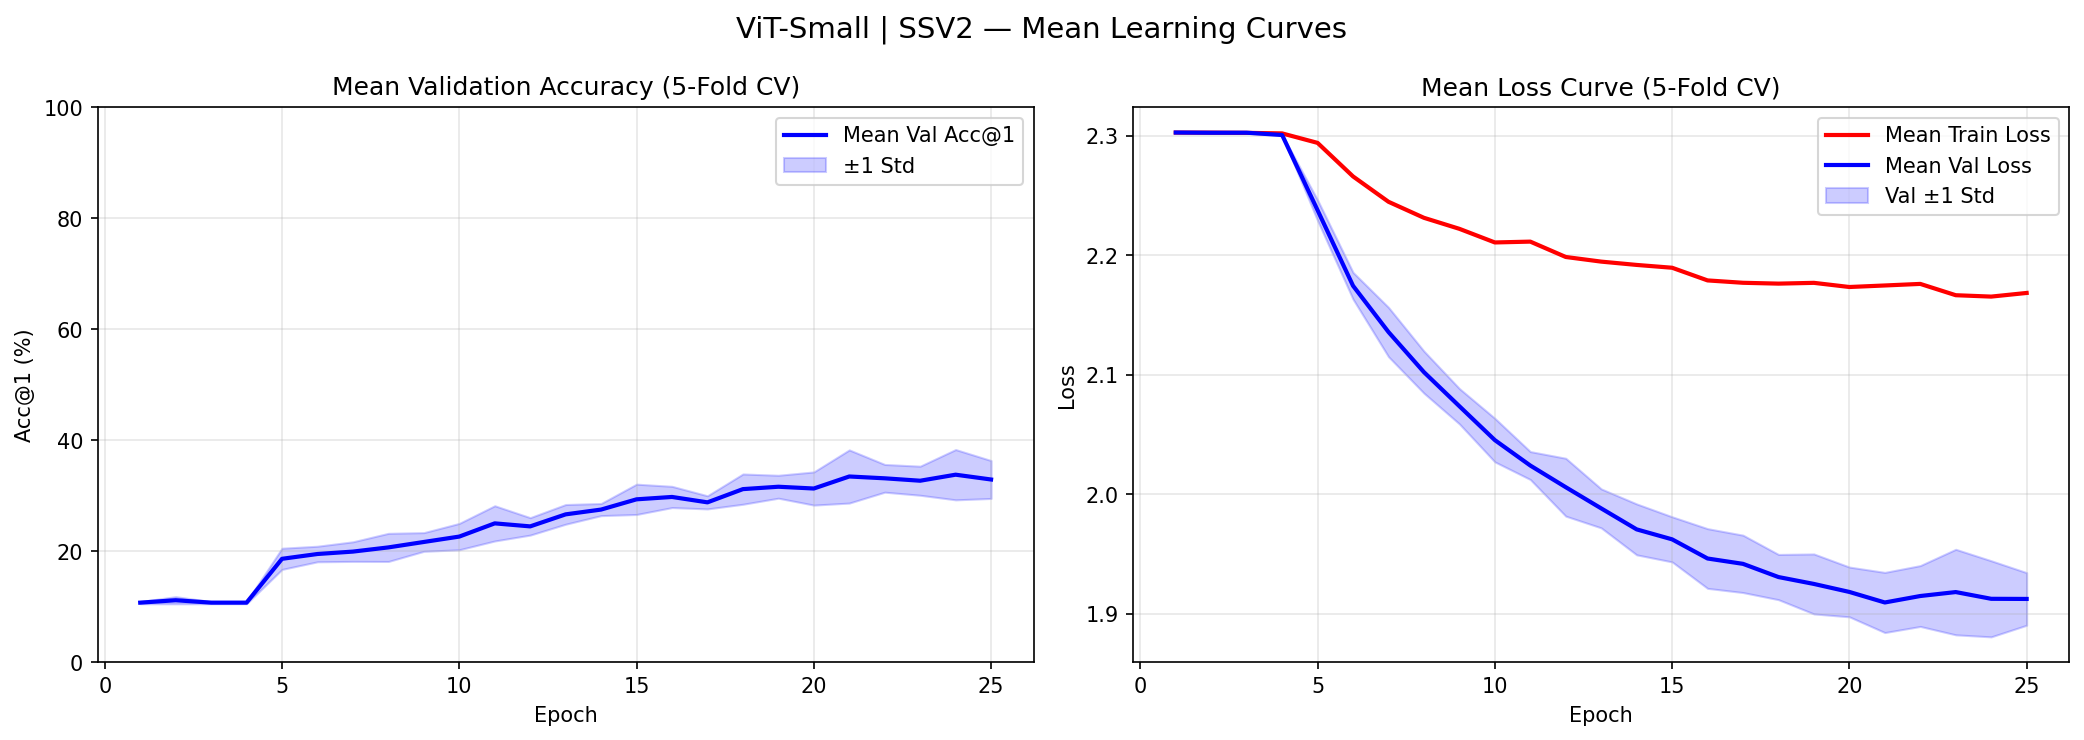
\includegraphics[width=0.95\textwidth]{figure/lc_vits_ssv2.png}
\caption{Kurva pelatihan rata-rata eksperimen E3 (ViT-Small + SSV2)}
\label{fig:4.lc_e3}
\end{figure}

Kurva pelatihan pada Gambar~\ref{fig:4.lc_e3} memperlihatkan pola konvergensi yang cukup stabil pada eksperimen E3. Akurasi validasi meningkat secara bertahap pada \textit{epoch-epoch} awal kemudian mulai melandai, mengindikasikan bahwa model berhasil mempelajari representasi fitur dari dataset SIBI meskipun kapasitas datanya terbatas. Terdapat fluktuasi pada nilai akurasi validasi antarfold yang mencerminkan variabilitas distribusi data antar lipatan, namun tren keseluruhan tetap menunjukkan peningkatan. \textit{Training loss} turun secara konsisten tanpa tanda-tanda divergensi, yang menandakan bahwa proses optimisasi berlangsung dengan baik. Dibandingkan dengan E1 dan E2 yang menggunakan K400, kurva E3 cenderung konvergen ke nilai yang lebih tinggi, memvalidasi keunggulan domain SSV2 untuk tugas pengenalan gestur tangan.\par

Tabel~\ref{tab:4.s1_perkelas} menyajikan laporan klasifikasi per kelas gabungan seluruh fold untuk keempat konfigurasi. Metrik presisi, \textit{recall}, dan F1-\textit{score} dihitung berdasarkan seluruh prediksi pada data validasi lintas lima fold.\par

\begin{table}[H]
\centering
\caption{Laporan klasifikasi per kelas (gabungan semua fold): E1--E4}
\label{tab:4.s1_perkelas}
{\setlength{\tabcolsep}{3pt}
\footnotesize
\resizebox{\linewidth}{!}{%
\begin{tabular}{|l|>{\centering\arraybackslash}p{0.6cm}|>{\centering\arraybackslash}p{0.6cm}|>{\centering\arraybackslash}p{0.6cm}|>{\centering\arraybackslash}p{0.6cm}|>{\centering\arraybackslash}p{0.6cm}|>{\centering\arraybackslash}p{0.6cm}|>{\centering\arraybackslash}p{0.6cm}|>{\centering\arraybackslash}p{0.6cm}|>{\centering\arraybackslash}p{0.6cm}|>{\centering\arraybackslash}p{0.6cm}|>{\centering\arraybackslash}p{0.6cm}|>{\centering\arraybackslash}p{0.6cm}|}
\hline
\rowcolor{gray!15} \multicolumn{1}{|c|}{\multirow{2}{*}{\textbf{Kelas}}} & \multicolumn{3}{c|}{\cellcolor{gray!15}\textbf{E1 (ViT-S + K400)}} & \multicolumn{3}{c|}{\cellcolor{gray!15}\textbf{E2 (ViT-B + K400)}} & \multicolumn{3}{c|}{\cellcolor{gray!15}\textbf{E3 (ViT-S + SSV2)}} & \multicolumn{3}{c|}{\cellcolor{gray!15}\textbf{E4 (ViT-B + SSV2)}} \\
\cline{2-13}
 & \multicolumn{1}{c|}{$P$} & \multicolumn{1}{c|}{$R$} & \multicolumn{1}{c|}{$F_1$} & \multicolumn{1}{c|}{$P$} & \multicolumn{1}{c|}{$R$} & \multicolumn{1}{c|}{$F_1$} & \multicolumn{1}{c|}{$P$} & \multicolumn{1}{c|}{$R$} & \multicolumn{1}{c|}{$F_1$} & \multicolumn{1}{c|}{$P$} & \multicolumn{1}{c|}{$R$} & \multicolumn{1}{c|}{$F_1$} \\
\hline
Aku     & 0.00 & 0.00 & 0.00 & 0.00 & 0.00 & 0.00 & 0.38 & 0.06 & 0.10 & 0.00 & 0.00 & 0.00 \\
Bapak   & 0.27 & 0.28 & 0.27 & 0.20 & 0.77 & 0.32 & 0.30 & 0.57 & 0.39 & 0.27 & 0.58 & 0.37 \\
Bawa    & 0.42 & 0.95 & 0.59 & 0.56 & 0.99 & 0.72 & 0.49 & 0.93 & 0.64 & 0.48 & 0.88 & 0.62 \\
Guru    & 0.00 & 0.00 & 0.00 & 0.50 & 0.01 & 0.02 & 0.70 & 0.31 & 0.43 & 0.70 & 0.08 & 0.14 \\
Ibu     & 0.16 & 0.67 & 0.26 & 0.28 & 0.18 & 0.22 & 0.19 & 0.33 & 0.24 & 0.23 & 0.46 & 0.31 \\
Kamu    & 0.00 & 0.00 & 0.00 & 0.14 & 0.20 & 0.17 & 0.29 & 0.09 & 0.13 & 0.18 & 0.17 & 0.17 \\
Mau     & 0.24 & 0.22 & 0.23 & 0.38 & 0.20 & 0.26 & 0.20 & 0.27 & 0.23 & 0.21 & 0.25 & 0.23 \\
Pulang  & 0.21 & 0.15 & 0.18 & 0.39 & 0.29 & 0.33 & 0.46 & 0.22 & 0.30 & 0.31 & 0.18 & 0.23 \\
Sekolah & 0.15 & 0.09 & 0.11 & 0.27 & 0.22 & 0.24 & 0.20 & 0.19 & 0.20 & 0.25 & 0.20 & 0.22 \\
Suka    & 0.36 & 0.04 & 0.08 & 0.29 & 0.08 & 0.12 & 0.34 & 0.24 & 0.28 & 0.16 & 0.06 & 0.08 \\
\hline
\textit{Macro} Avg & 0.18 & 0.24 & 0.17 & 0.30 & 0.29 & 0.24 & 0.35 & 0.32 & 0.29 & 0.28 & 0.29 & 0.24 \\
\hline
\end{tabular}%
}
}
\end{table}

Analisis per kelas pada Tabel~\ref{tab:4.s1_perkelas} mengungkapkan beberapa pola yang konsisten di seluruh konfigurasi. Kelas \textit{Bawa} secara konsisten memiliki \textit{recall} tertinggi di semua model (0.88--0.99), mengindikasikan bahwa gestur ``Bawa'' memiliki karakteristik visual yang paling mudah dikenali oleh model karena gerakan tangannya yang distingtif dan konsisten antar penutur. Sebaliknya, kelas \textit{Aku} hampir tidak dapat dikenali oleh tiga dari empat konfigurasi (F1 mendekati nol pada E1, E2, dan E4), kemungkinan disebabkan oleh kemiripan visual gestur ini dengan kelas lain atau tingginya variasi antar penutur. Eksperimen E3 menunjukkan keunggulan pada kelas \textit{Guru} (F1 0.43 vs. 0.00--0.14 pada konfigurasi lain) dan \textit{Suka} (F1 0.28 vs. 0.08--0.12), mengindikasikan bahwa representasi spasio-temporal dari SSV2 membantu model menangkap pola temporal yang lebih halus pada gestur-gestur tersebut. Kelas \textit{Kamu} tetap sulit dikenali di semua konfigurasi (F1 0.00--0.17), yang mungkin disebabkan oleh ambiguitas visual antara gestur ini dengan beberapa kelas lainnya. Pola asimetri presisi-\textit{recall} pada E2 untuk kelas \textit{Guru} (P=0.50, R=0.01) menunjukkan bahwa ViT-Base dengan K400 hanya mampu memprediksi kelas ini dalam kasus yang sangat jelas, sementara mayoritas sampel ``Guru'' salah diklasifikasikan sebagai kelas lain.\par
Analisis per kelas pada Tabel~\ref{tab:4.s1_perkelas} mengungkapkan beberapa pola yang konsisten di seluruh konfigurasi. Kelas \textit{Bawa} secara konsisten memiliki \textit{recall} tertinggi di semua model (0.88--0.99), mengindikasikan bahwa gestur ``Bawa'' memiliki karakteristik visual yang paling mudah dikenali oleh model karena gerakan tangannya yang distingtif dan konsisten antarpenutur. Sebaliknya, kelas \textit{Aku} hampir tidak dapat dikenali oleh tiga dari empat konfigurasi (F1 mendekati nol pada E1, E2, dan E4), kemungkinan disebabkan oleh kemiripan visual gestur ini dengan kelas lain atau tingginya variasi antarpenutur. Eksperimen E3 menunjukkan keunggulan pada kelas \textit{Guru} (F1 0.43 vs. 0.00--0.14 pada konfigurasi lain) dan \textit{Suka} (F1 0.28 vs. 0.08--0.12), mengindikasikan bahwa representasi spasio-temporal dari SSV2 membantu model menangkap pola temporal yang lebih halus pada gestur-gestur tersebut. Kelas \textit{Kamu} tetap sulit dikenali di semua konfigurasi (F1 0.00--0.17), yang mungkin disebabkan oleh ambiguitas visual antara gestur ini dengan beberapa kelas lainnya. Pola asimetri presisi-\textit{recall} pada E2 untuk kelas \textit{Guru} (P=0.50, R=0.01) menunjukkan bahwa ViT-Base dengan K400 hanya mampu memprediksi kelas ini dalam kasus yang sangat jelas, sementara mayoritas sampel ``Guru'' salah diklasifikasikan sebagai kelas lain.\par

Gambar~\ref{fig:4.cm_e3} menampilkan \textit{confusion matrix} gabungan seluruh fold untuk eksperimen E3 yang merupakan konfigurasi terbaik.\par

\begin{figure}[H]
\centering
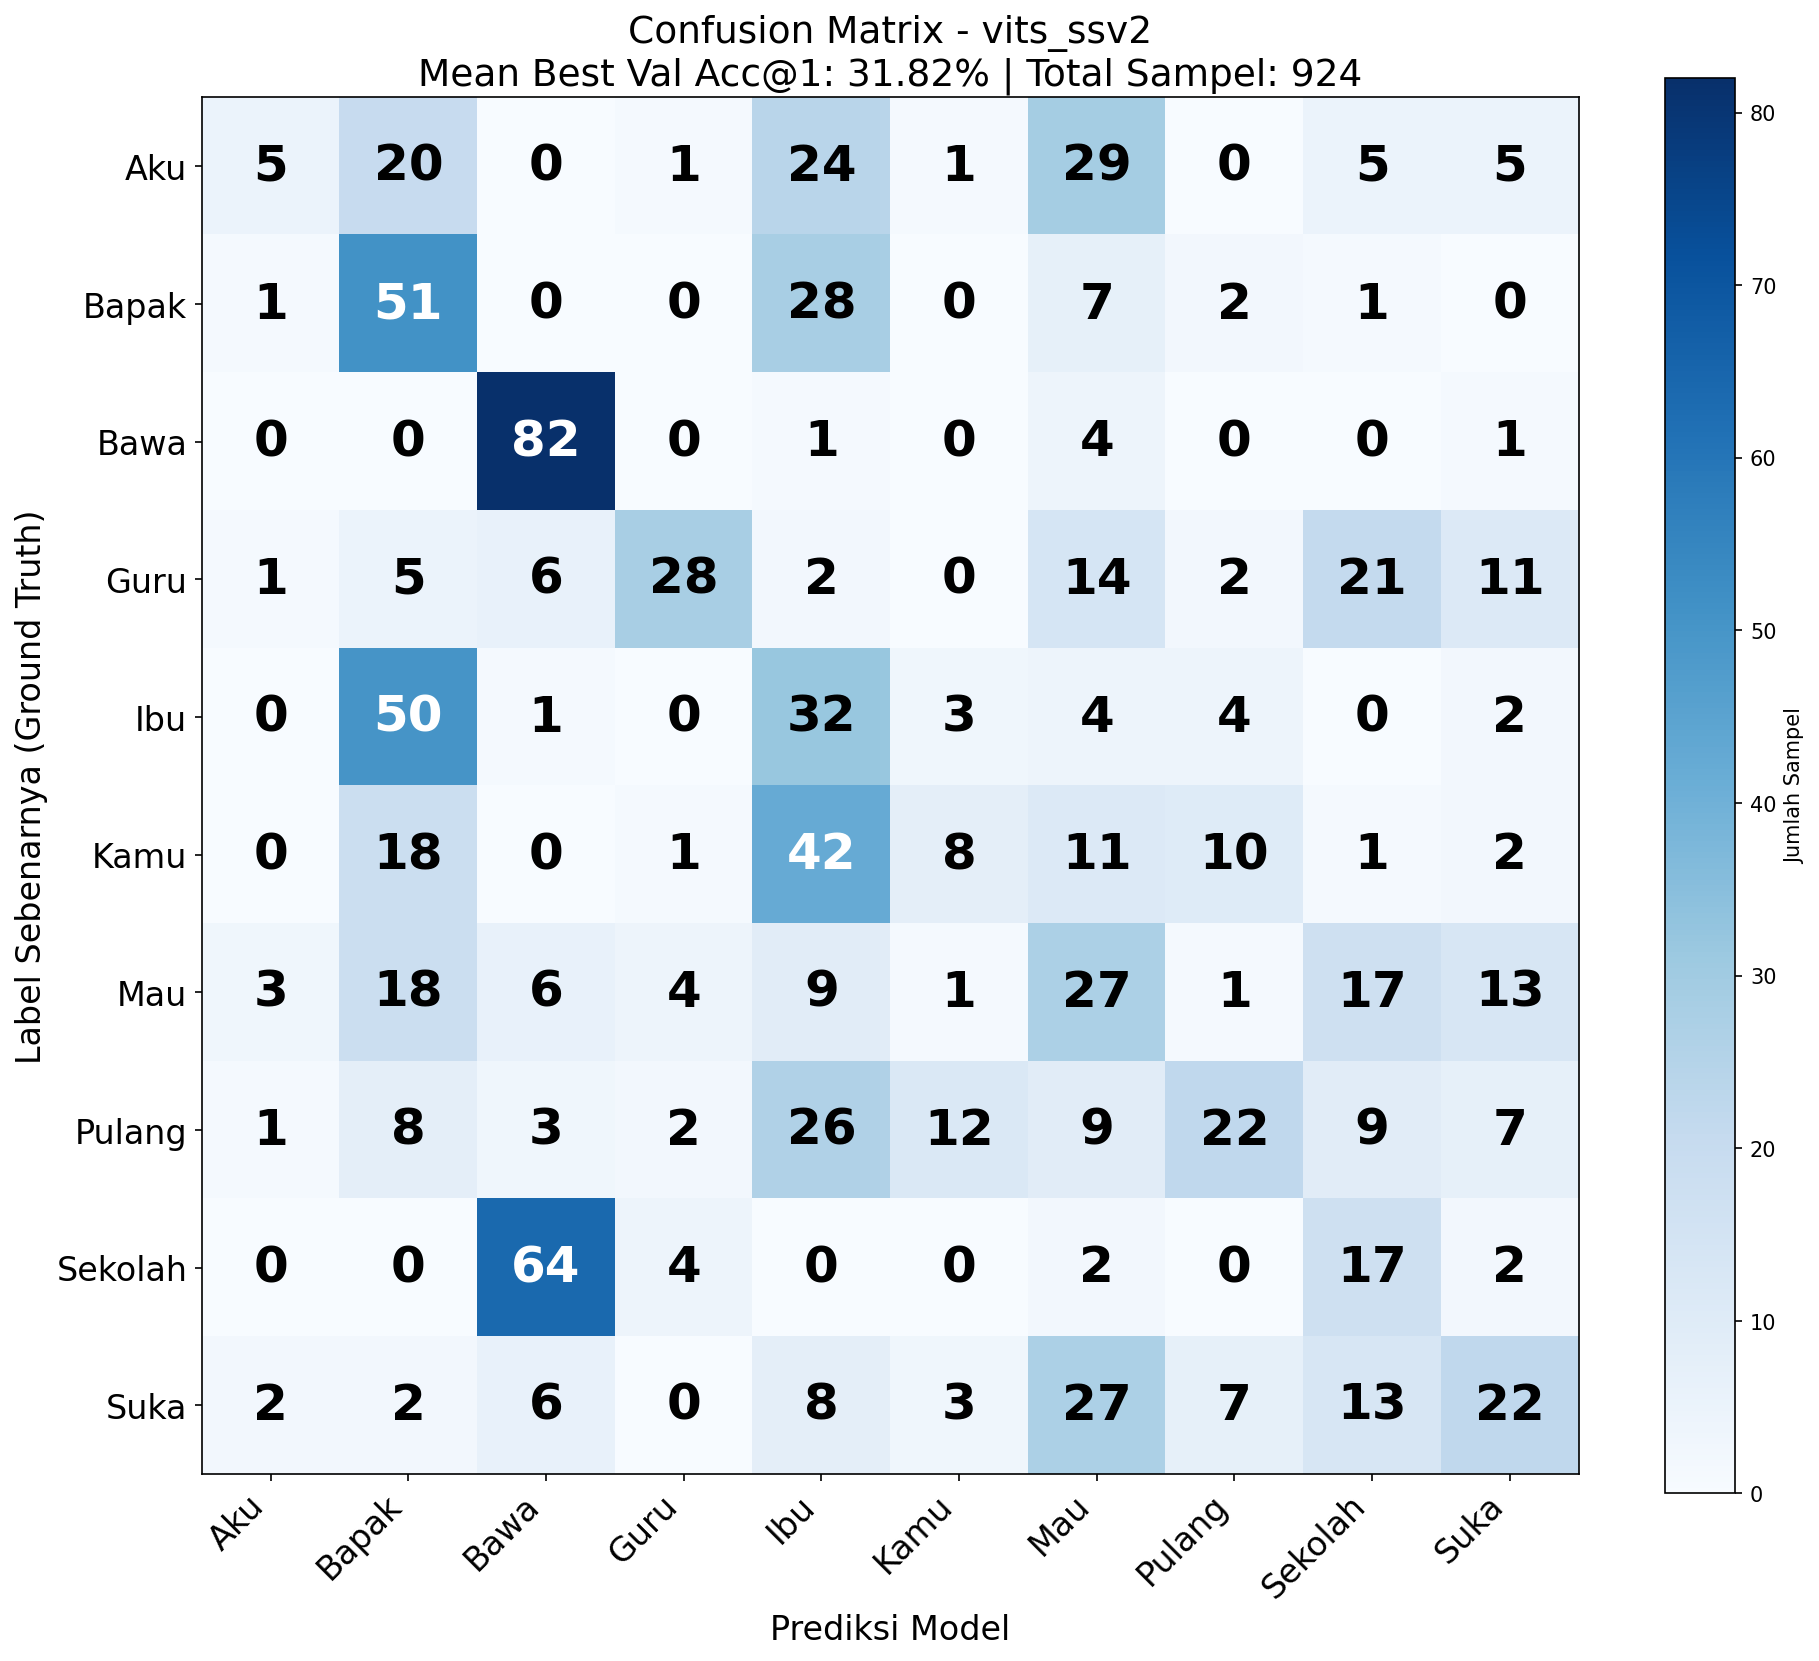
\includegraphics[width=0.95\textwidth]{figure/cm_vits_ssv2_new_font.png}
\caption{\textit{Confusion matrix} gabungan semua fold eksperimen E3 (ViT-Small + SSV2)}
\label{fig:4.cm_e3}
\end{figure}

\textit{Confusion matrix} pada Gambar~\ref{fig:4.cm_e3} memperlihatkan bahwa diagonal utama memiliki intensitas yang relatif rendah, mencerminkan akurasi keseluruhan yang masih terbatas. Kelas \textit{Bawa} menunjukkan nilai diagonal yang paling tinggi dengan prediksi yang hampir sempurna pada kolom tersebut, mengonfirmasi \textit{recall} tinggi yang terlihat pada Tabel~\ref{tab:4.s1_perkelas}. Terdapat pola kesalahan yang signifikan pada baris kelas \textit{Aku}, di mana hampir seluruh sampel diprediksi sebagai kelas lain terutama \textit{Bapak} dan \textit{Kamu} mengindikasikan adanya kemiripan temporal antara ketiga gestur tersebut yang sulit dibedakan oleh model. Kelas \textit{Mau} dan \textit{Pulang} juga menunjukkan distribusi kesalahan yang menyebar ke berbagai kelas, yang kemungkinan disebabkan oleh variasi inter-penutur yang tinggi pada kedua gestur ini sehingga representasi fiturnya kurang terpusat. Secara umum, \textit{confusion matrix} E3 menunjukkan distribusi kesalahan yang lebih merata dibandingkan E1 dan E2 yang cenderung memiliki satu atau dua kelas dominan sebagai target prediksi salah, yang mengindikasikan bahwa E3 memiliki kemampuan diskriminasi yang lebih baik secara keseluruhan.\par
\textit{Confusion matrix} pada Gambar~\ref{fig:4.cm_e3} memperlihatkan bahwa diagonal utama memiliki intensitas yang relatif rendah, mencerminkan akurasi keseluruhan yang masih terbatas. Kelas \textit{Bawa} menunjukkan nilai diagonal yang paling tinggi dengan prediksi yang hampir sempurna pada kolom tersebut, mengonfirmasi \textit{recall} tinggi yang terlihat pada Tabel~\ref{tab:4.s1_perkelas}. Terdapat pola kesalahan yang signifikan pada baris kelas \textit{Aku}, di mana hampir seluruh sampel diprediksi sebagai kelas lain terutama \textit{Bapak} dan \textit{Kamu} mengindikasikan adanya kemiripan temporal antara ketiga gestur tersebut yang sulit dibedakan oleh model. Kelas \textit{Mau} dan \textit{Pulang} juga menunjukkan distribusi kesalahan yang menyebar ke berbagai kelas, yang kemungkinan disebabkan oleh variasi interpenutur yang tinggi pada kedua gestur ini sehingga representasi fiturnya kurang terpusat. Secara umum, \textit{confusion matrix} E3 menunjukkan distribusi kesalahan yang lebih merata dibandingkan E1 dan E2 yang cenderung memiliki satu atau dua kelas dominan sebagai target prediksi salah, yang mengindikasikan bahwa E3 memiliki kemampuan diskriminasi yang lebih baik secara keseluruhan.\par

Berdasarkan seluruh hasil pada bagian ini, konfigurasi E3 (ViT-Small + SSV2) ditetapkan sebagai konfigurasi terbaik dan menjadi dasar bagi eksperimen pada bagian selanjutnya.\par


%===========================================================================
\subsection{Perbandingan Strategi Pelatihan \textit{Pre-train} dan \textit{Scratch}} \label{IV.Sek2}
%===========================================================================

Bagian ini mengevaluasi dampak bobot \textit{pre-train} VideoMAE terhadap performa akhir model dengan membandingkan tiga strategi pelatihan menggunakan \textit{backbone} ViT-Small dan dataset SSV2. Strategi \textit{two-stage pre-train} menggunakan bobot pra-latih SSV2 sebagai titik awal, kemudian dilatih dalam dua tahap: \textit{stage} 1 dengan \textit{learning rate} tinggi ($10^{-3}$, 5 epoch) untuk adaptasi cepat, dilanjutkan \textit{stage} 2 dengan \textit{learning rate} rendah ($10^{-5}$, 50 epoch) untuk penyempurnaan. Sebaliknya, strategi \textit{scratch} melatih model dari bobot yang diinisialisasi secara acak. Konfigurasi lengkap disajikan pada Tabel~\ref{tab:4.s2_config}.\par

\begin{table}[H]
\centering
\caption{Konfigurasi eksperimen perbandingan strategi pelatihan}
\label{tab:4.s2_config}
{\setlength{\tabcolsep}{3pt}
\footnotesize
\begin{tabular}{|l|l|l|l|}
\hline
\rowcolor{gray!15} \multicolumn{1}{|c|}{\textbf{Parameter}} & \multicolumn{1}{c|}{\textbf{E5}} & \multicolumn{1}{c|}{\textbf{E6}} & \multicolumn{1}{c|}{\textbf{E7}} \\
\hline
Strategi Pelatihan & \makecell[l]{\textit{Two-Stage}\\\textit{Pre-train}} & \makecell[l]{\textit{Two-Stage}\\\textit{Scratch}} & \makecell[l]{\textit{Single-Stage}\\\textit{Scratch}} \\
\hline
Inisialisasi & Bobot SSV2 & Acak & Acak \\
\hline
\textit{Epoch Stage} 1 & \multicolumn{1}{r|}{5} & \multicolumn{1}{r|}{5} & {--} \\
\hline
\textit{Epoch Stage} 2 & \multicolumn{1}{r|}{50} & \multicolumn{1}{r|}{50} & \multicolumn{1}{r|}{50} \\
\hline
\textit{Learning Rate Stage} 1 & \multicolumn{1}{r|}{$10^{-3}$} & \multicolumn{1}{r|}{$10^{-3}$} & {--} \\
\hline
\textit{Learning Rate Stage} 2 & \multicolumn{1}{r|}{$10^{-5}$} & \multicolumn{1}{r|}{$10^{-5}$} & \multicolumn{1}{r|}{$10^{-3}$} \\
\hline
\textit{Batch Size} & \multicolumn{1}{r|}{16} & \multicolumn{1}{r|}{16} & \multicolumn{1}{r|}{16} \\
\hline
\textit{Hyperparameter} Lain & \multicolumn{3}{l|}{Sama dengan Tabel~\ref{tab:4.umum_config}} \\
\hline
\end{tabular}
}
\end{table}

Pemilihan hiperparameter pada strategi \textit{two-stage pre-train} didasarkan pada peran masing-masing tahap yang berbeda secara fundamental. Pada \textit{stage} 1, seluruh lapisan \textit{backbone} (encoder Transformer) dibekukan (\textit{frozen}) sehingga hanya bobot \textit{classification head}, sebuah lapisan linear yang diinisialisasi secara acak, yang diperbarui. Karena \textit{head} belum memiliki representasi awal yang bermakna, \textit{learning rate} tinggi $10^{-3}$ diperlukan agar lapisan ini dapat konvergen dengan cepat. Dengan \textit{backbone} dalam kondisi beku, penggunaan LR tinggi tidak berisiko merusak representasi fitur yang telah dipelajari selama \textit{pre-training} SSV2. Durasi 5 epoch dipilih karena \textit{classification head} hanya terdiri dari satu lapisan linear dengan jumlah parameter yang kecil, sehingga nilai epoch yang lebih banyak tidak memberikan manfaat tambahan dan justru berisiko menyebabkan \textit{overfitting} pada fitur \textit{backbone} yang masih beku. Tujuan \textit{stage} 1 semata-mata adalah menginisialisasi \textit{head} dengan pemetaan kelas yang cukup baik sebagai titik awal \textit{stage} 2.

Pada \textit{stage} 2, seluruh lapisan dibebaskan (\textit{unfrozen}) dan model dilatih secara \textit{end-to-end}. \textit{Learning rate} yang jauh lebih kecil ($10^{-5}$) dipilih untuk mencegah \textit{catastrophic forgetting}, fenomena di mana pembaruan gradien yang terlalu besar menghapus representasi berharga yang telah dibangun selama \textit{pre-training} SSV2. Dengan LR kecil, bobot \textit{backbone} teradaptasi secara bertahap terhadap karakteristik spasio-temporal gestur SIBI tanpa kehilangan kemampuan ekstraksi fitur gerak yang diperoleh dari SSV2. Durasi 50 epoch dipilih agar proses penyempurnaan ini memiliki waktu yang cukup untuk konvergen secara menyeluruh.\par

\begin{table}[H]
\centering
\caption{Nilai \textit{Best Val Acc@1} (\%) per fold dan ringkasan hasil eksperimen E5--E7}
\label{tab:4.s2_fold}
{\setlength{\tabcolsep}{3pt}
\footnotesize
\begin{tabular}{|l|r|r|r|r|r|r|r|}
\hline
\rowcolor{gray!15} \multicolumn{1}{|c|}{\textbf{Kode}} & \multicolumn{1}{c|}{\textbf{Fold 1}} & \multicolumn{1}{c|}{\textbf{Fold 2}} & \multicolumn{1}{c|}{\textbf{Fold 3}} & \multicolumn{1}{c|}{\textbf{Fold 4}} & \multicolumn{1}{c|}{\textbf{Fold 5}} & \multicolumn{1}{c|}{\makecell[c]{\textbf{Rata-}\\\textbf{rata}}} & \multicolumn{1}{c|}{\textbf{Terbaik}} \\
\hline
\rowcolor{highlightgreen}E5 & 62.16 & 63.59 & 62.16 & 70.27 & 61.08 & 63.85 & 70.27 \\
\hline
\rowcolor{highlightpink}E6 & 10.27 & 10.33 & 12.43 & 12.43 & 11.35 & 11.36 & 12.43 \\
\hline
E7 & 11.35 & 13.04 & 11.35 & 11.89 & 12.43 & 12.01 & 13.04 \\
\hline
\end{tabular}
}
\end{table}

Tabel~\ref{tab:4.s2_fold} menunjukkan kesenjangan performa yang sangat besar antara strategi \textit{pre-train} (E5) dan kedua strategi \textit{scratch} (E6, E7). Eksperimen E5 mencapai rata-rata akurasi 63.85\%, meningkat 28.67 poin persentase dari \textit{baseline} E3, sementara E6 dan E7 hanya menghasilkan akurasi di kisaran 11--13\%, yang praktis tidak berbeda dari prediksi acak untuk 10 kelas (10\%). Konsistensi performa E5 di seluruh fold (61--70\%) berbanding terbalik dengan E6 dan E7 yang stagnan di angka rendah tanpa variasi berarti antar fold. Perbandingan E6 (\textit{two-stage scratch}) dan E7 (\textit{single-stage scratch}) yang hampir setara (11.36\% vs. 12.01\%) mengindikasikan bahwa skema pelatihan dua tahap tidak otomatis memberi manfaat jika \textit{backbone} belum memiliki representasi yang bermakna. Keunggulan E5 tidak hanya berasal dari bobot \textit{pre-train} SSV2, tetapi juga dari tahap \textit{linear probing} pada \textit{stage} 1 yang lebih dahulu menyesuaikan \textit{classification head} ke kelas-kelas SIBI sebelum \textit{fine-tuning} penuh dilakukan. Sebaliknya, pada E6, \textit{linear probing} diterapkan di atas \textit{backbone} acak yang dibekukan, sehingga \textit{head} hanya menerima fitur yang belum informatif dan tidak memperoleh titik awal yang kuat untuk \textit{stage} 2.\par
Tabel~\ref{tab:4.s2_fold} menunjukkan kesenjangan performa yang sangat besar antara strategi \textit{pre-train} (E5) dan kedua strategi \textit{scratch} (E6, E7). Eksperimen E5 mencapai rata-rata akurasi 63.85\%, meningkat 28.67 poin persentase dari \textit{baseline} E3, sementara E6 dan E7 hanya menghasilkan akurasi di kisaran 11--13\%, yang praktis tidak berbeda dari prediksi acak untuk 10 kelas (10\%). Konsistensi performa E5 di seluruh fold (61--70\%) berbanding terbalik dengan E6 dan E7 yang stagnan di angka rendah tanpa variasi berarti antarfold. Perbandingan E6 (\textit{two-stage scratch}) dan E7 (\textit{single-stage scratch}) yang hampir setara (11.36\% vs. 12.01\%) mengindikasikan bahwa skema pelatihan dua tahap tidak otomatis memberi manfaat jika \textit{backbone} belum memiliki representasi yang bermakna. Keunggulan E5 tidak hanya berasal dari bobot \textit{pre-train} SSV2, tetapi juga dari tahap \textit{linear probing} pada \textit{stage} 1 yang lebih dahulu menyesuaikan \textit{classification head} ke kelas-kelas SIBI sebelum \textit{fine-tuning} penuh dilakukan. Sebaliknya, pada E6, \textit{linear probing} diterapkan di atas \textit{backbone} acak yang dibekukan, sehingga \textit{head} hanya menerima fitur yang belum informatif dan tidak memperoleh titik awal yang kuat untuk \textit{stage} 2.\par

Gambar~\ref{fig:4.lc_e5} menampilkan kurva pelatihan rata-rata eksperimen E5 (\textit{two-stage pre-train}).\par

\begin{figure}[H]
\centering
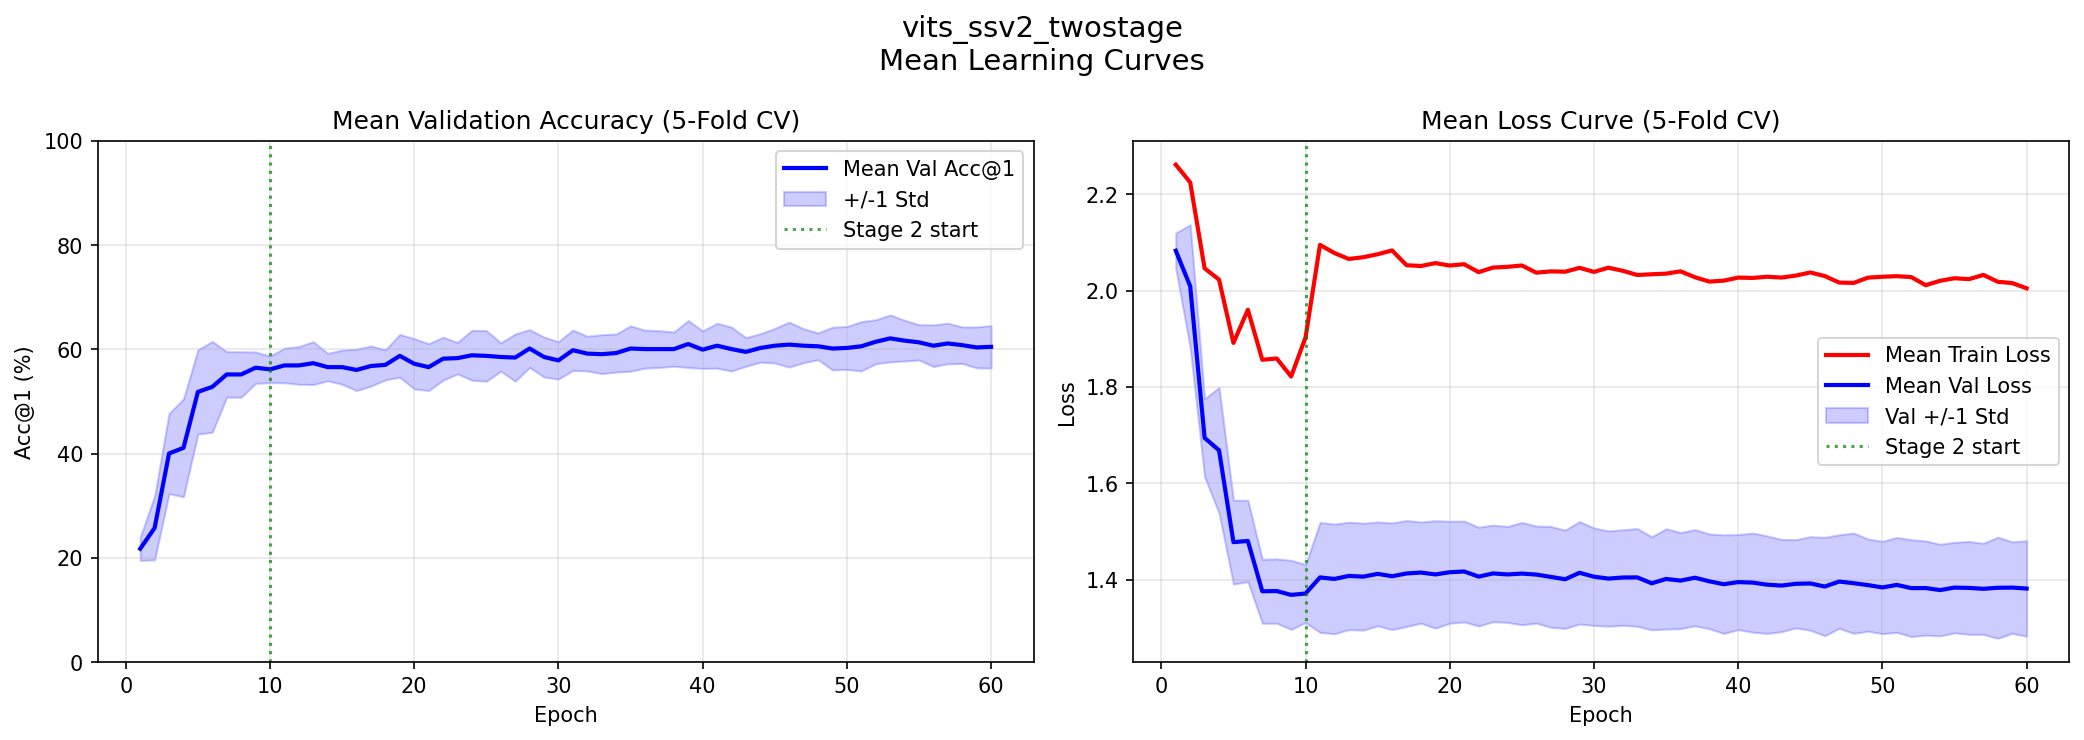
\includegraphics[width=0.95\textwidth]{figure/lc_vits_ssv2_twostage.png}
\caption{Kurva pelatihan rata-rata eksperimen E5 (\textit{Two-Stage Pre-train})}
\label{fig:4.lc_e5}
\end{figure}

Kurva pelatihan E5 pada Gambar~\ref{fig:4.lc_e5} menunjukkan konvergensi yang cepat dan stabil sejak epoch-epoch awal \textit{stage} 2, dengan akurasi validasi yang meningkat pesat hingga epoch ke-20 kemudian melandai secara bertahap. Stabilitas ini menunjukkan kombinasi dua faktor yang saling melengkapi: representasi \textit{pretrained} dari SSV2 sudah cukup relevan untuk domain gestur, dan tahap \textit{linear probing} pada \textit{stage} 1 membuat \textit{classification head} tidak memulai adaptasi dari kondisi acak ketika masuk ke \textit{stage} 2. Dengan demikian, kapasitas pelatihan dapat langsung difokuskan pada penyesuaian representasi spasio-temporal yang sudah ada terhadap karakteristik SIBI, bukan pada pencarian pemetaan kelas dari awal. Nilai akurasi validasi pada semua fold bergerak dalam rentang yang relatif konsisten (kurang lebih 61--70\%), mengindikasikan bahwa model tidak bergantung pada fold tertentu untuk menghasilkan performa yang baik. Tidak terlihat tanda-tanda \textit{overfitting} pada kurva ini, yang ditunjukkan oleh tidak adanya divergensi antara tren peningkatan \textit{training} dan \textit{validation}.\par

Gambar~\ref{fig:4.lc_e6} dan Gambar~\ref{fig:4.lc_e7} menampilkan kurva pelatihan eksperimen E6 dan E7 sebagai pembanding.\par

\begin{figure}[H]
\centering
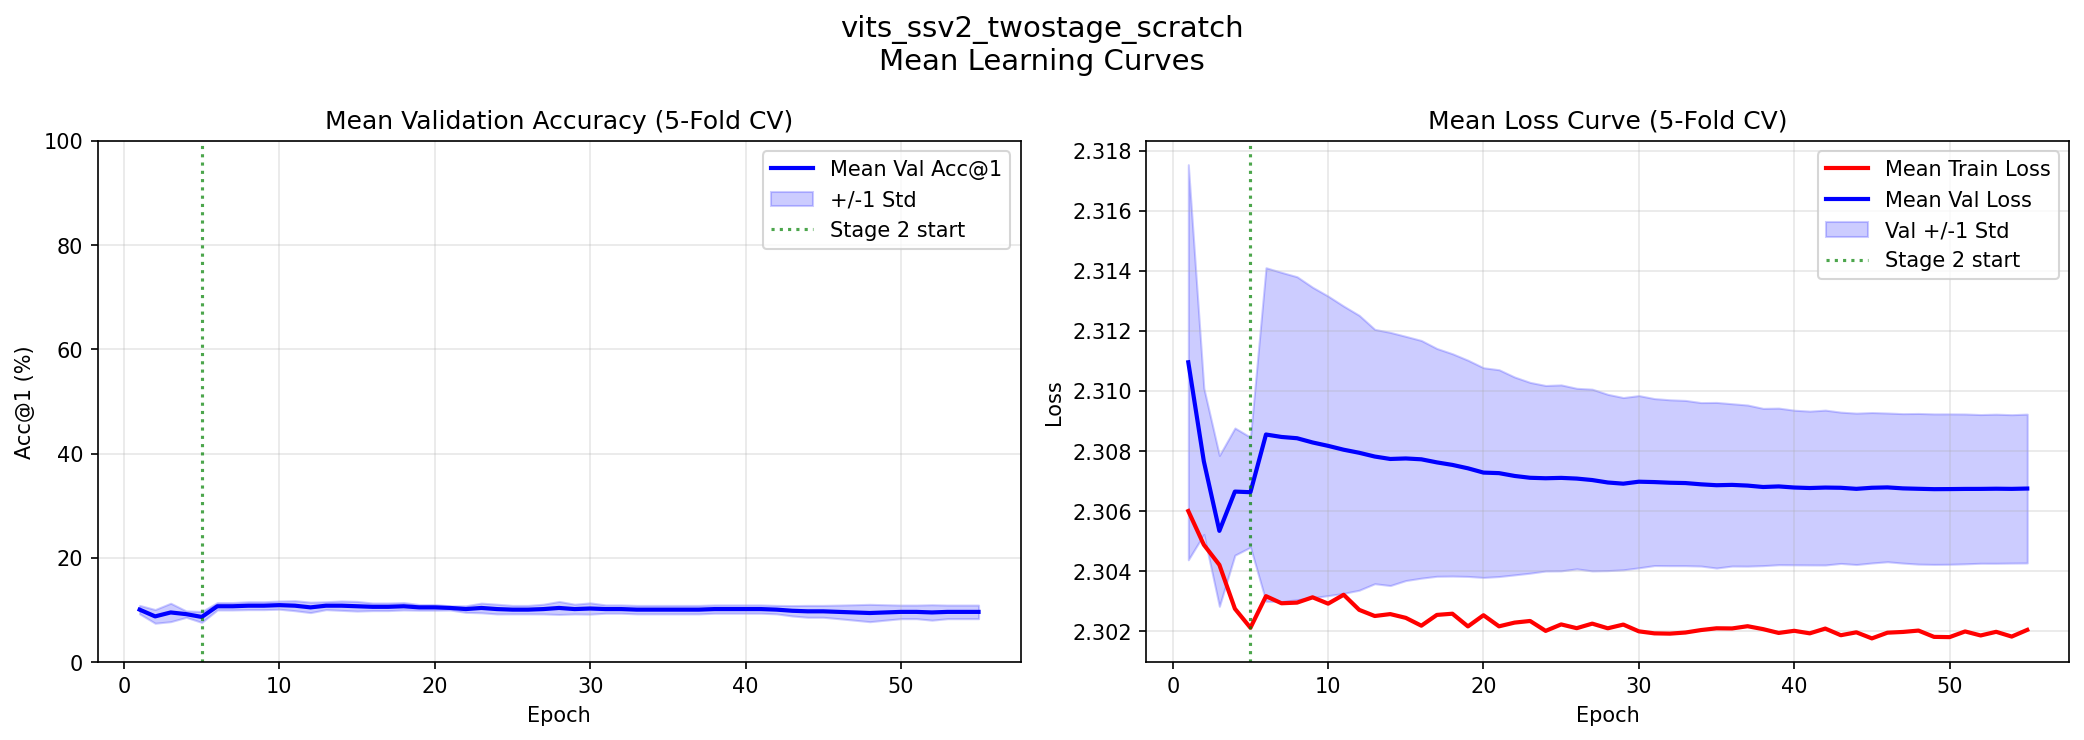
\includegraphics[width=0.95\textwidth]{figure/lc_vits_ssv2_twostage_scratch.png}
\caption{Kurva pelatihan rata-rata eksperimen E6 (\textit{Two-Stage Scratch})}
\label{fig:4.lc_e6}
\end{figure}

Kurva pelatihan E6 pada Gambar~\ref{fig:4.lc_e6} memperlihatkan pola yang sama sekali berbeda dari E5: akurasi validasi hampir tidak bergerak dari kisaran awal acak (~10\%) sepanjang 50 epoch pelatihan. \textit{Loss} pelatihan memang menurun secara bertahap, namun penurunan tersebut tidak berhasil diterjemahkan menjadi peningkatan kemampuan klasifikasi pada data validasi. Temuan ini penting karena menunjukkan bahwa keberadaan \textit{linear probing} saja belum cukup; pada E6, \textit{stage} 1 memang melatih \textit{head} lebih dahulu, tetapi \textit{head} tersebut bertumpu pada keluaran \textit{backbone} acak yang dibekukan sehingga ruang fitur yang dipelajari tetap lemah. Saat masuk ke \textit{stage} 2, model tetap tidak memiliki fondasi representasi yang stabil untuk dikembangkan. Dengan arsitektur VideoMAE yang berparameter besar dan dataset SIBI yang relatif terbatas, kondisi ini membuat gradien yang terbentuk tidak cukup konsisten untuk mendorong konvergensi yang bermakna. Karena itu, kegagalan E6 lebih tepat dipahami sebagai bukti bahwa \textit{linear probing} hanya efektif bila didukung representasi awal yang informatif, bukan sebagai akibat ketiadaan tahapan dua tahap semata.\par

\begin{figure}[H]
\centering
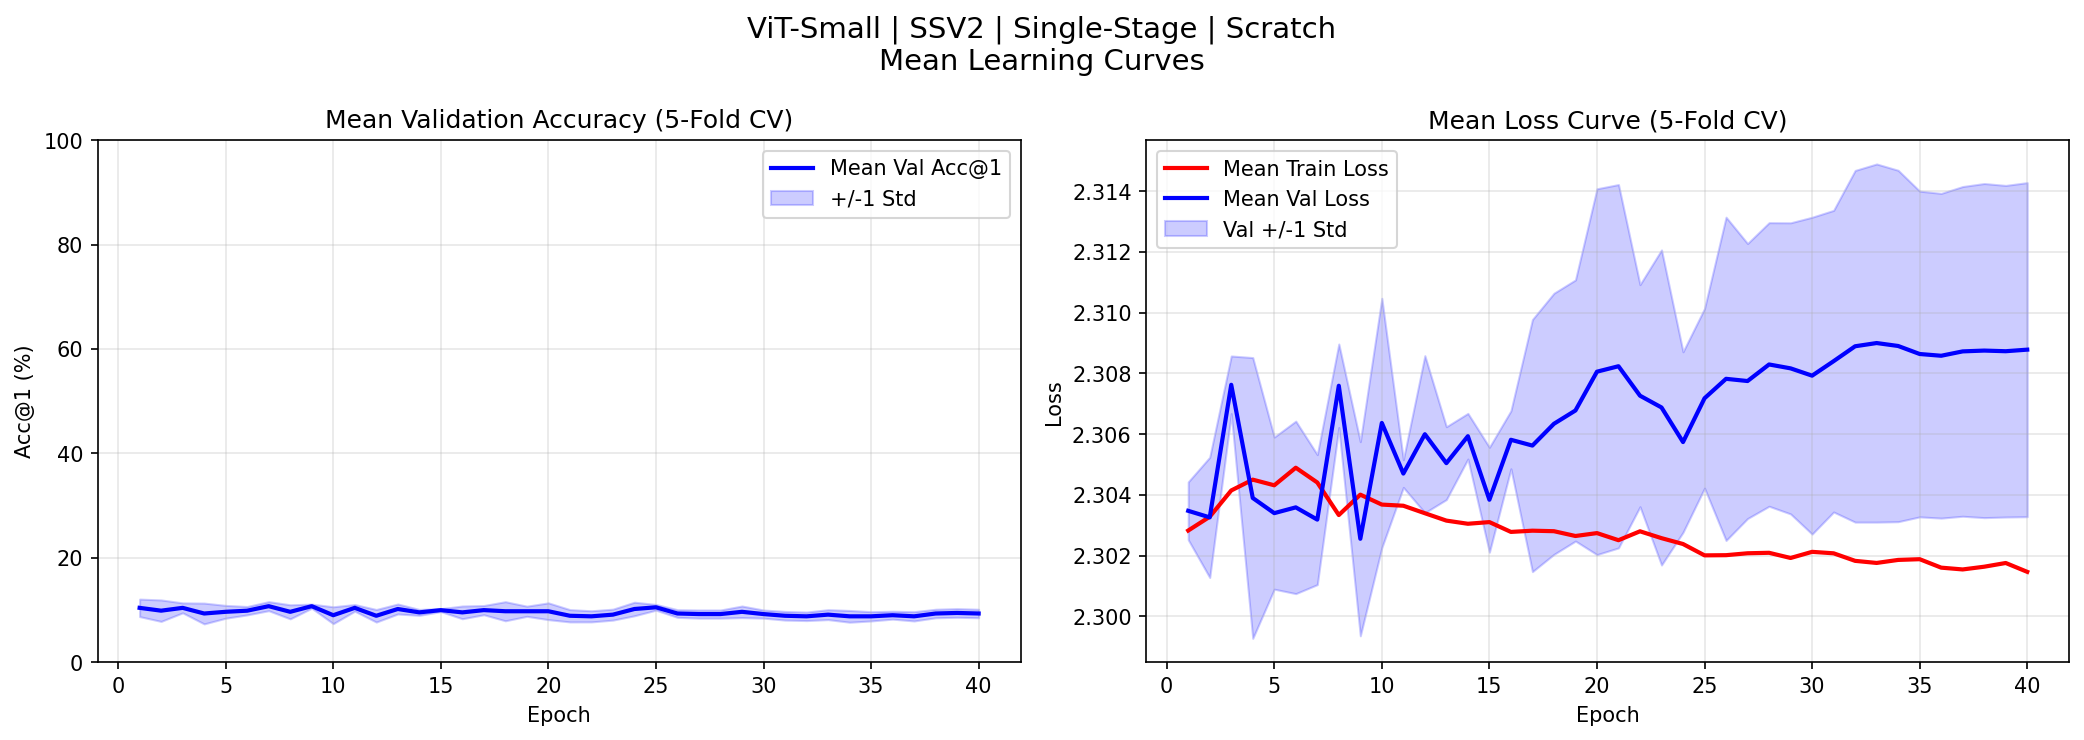
\includegraphics[width=0.95\textwidth]{figure/lc_vits_ssv2_singlestage_scratch.png}
\caption{Kurva pelatihan rata-rata eksperimen E7 (\textit{Single-Stage Scratch})}
\label{fig:4.lc_e7}
\end{figure}

Kurva E7 pada Gambar~\ref{fig:4.lc_e7} menunjukkan pola yang sangat mirip dengan E6, model gagal berkonvergensi dan akurasi validasi tetap berada di sekitar nilai acak sepanjang pelatihan. Meskipun E7 menggunakan \textit{learning rate} yang lebih tinggi ($10^{-3}$) dibandingkan \textit{stage} 2 E6 ($10^{-5}$), perbedaan ini tidak memberikan keuntungan berarti, model tetap tidak mampu mempelajari representasi diskriminatif dari data SIBI tanpa fondasi fitur awal yang informatif. Kemiripan kurva E6 dan E7 justru memperjelas posisi \textit{linear probing}: tahapan tersebut membantu pada E5 karena \textit{head} diadaptasikan di atas fitur \textit{pretrained} yang sudah kaya, tetapi pada E6 tidak cukup kuat untuk mengimbangi kelemahan \textit{backbone} acak. Dengan demikian, kegagalan kedua eksperimen \textit{scratch} ini bukan disebabkan oleh pilihan \textit{learning rate} semata, melainkan oleh absennya representasi awal yang dapat ditransfer ke tugas SIBI.\par

Perlu dicatat bahwa secara total, eksperimen E5 menjalani 55 epoch pelatihan (5 epoch \textit{stage} 1 ditambah 50 epoch \textit{stage} 2), sementara E7 hanya menjalani 50 epoch. Perbedaan 5 epoch ini tidak memengaruhi validitas perbandingan karena kurva pelatihan E7 telah menunjukkan kondisi stagnan sejak epoch-epoch awal, akurasi validasi tidak pernah meninggalkan kisaran nilai acak (10--13\%) sepanjang keseluruhan proses. Fenomena ini menunjukkan bahwa model telah mencapai batas kemampuannya jauh sebelum epoch ke-50, sehingga penambahan epoch dalam jumlah berapapun tidak akan mengubah kesimpulan. Hal ini dikuatkan pula oleh eksperimen E6 yang menggunakan skema dua tahap penuh (total 55 epoch) namun tetap menghasilkan akurasi yang setara dengan E7, keduanya gagal di angka yang sama tanpa memandang durasi atau skema pelatihan yang digunakan. Dengan demikian, perbandingan antara E5 dan E7 bersifat konklusif secara kualitatif, kesenjangan performa yang terlihat bukan merupakan artefak dari perbedaan jumlah epoch, melainkan mencerminkan perbedaan mendasar antara model yang diinisialisasi dengan representasi bermakna versus model yang diinisialisasi secara acak pada dataset berskala kecil.\par

Tabel~\ref{tab:4.s2_perkelas} menyajikan laporan klasifikasi per kelas untuk eksperimen E5. Eksperimen E6 dan E7 tidak dianalisis per kelas karena akurasi keduanya mendekati nilai acak sehingga metrik per kelas tidak mengandung informasi yang dapat diinterpretasikan secara bermakna.\par

\begin{table}[H]
\centering
\caption{Laporan klasifikasi per kelas (gabungan semua fold) eksperimen E5}
\label{tab:4.s2_perkelas}
{\setlength{\tabcolsep}{3pt}
\footnotesize
\begin{tabular}{|l|r|r|r|r|}
\hline
\rowcolor{gray!15} \multicolumn{1}{|c|}{Kelas} & \multicolumn{1}{c|}{Presisi} & \multicolumn{1}{c|}{\textit{Recall}} & \multicolumn{1}{c|}{F1-\textit{Score}} & \multicolumn{1}{c|}{\textit{Support}} \\
\hline
Aku     & 0.66 & 0.70 & 0.68 & 90 \\
Bapak   & 0.81 & 0.52 & 0.64 & 90 \\
Bawa    & 0.62 & 1.00 & 0.76 & 88 \\
Guru    & 0.79 & 0.84 & 0.82 & 90 \\
Ibu     & 0.54 & 0.86 & 0.66 & 96 \\
Kamu    & 0.60 & 0.60 & 0.60 & 93 \\
Mau     & 0.43 & 0.68 & 0.52 & 99 \\
Pulang  & 0.69 & 0.38 & 0.49 & 99 \\
Sekolah & 0.82 & 0.35 & 0.49 & 89 \\
Suka    & 0.58 & 0.21 & 0.31 & 90 \\
\hline
\textit{Macro} Avg & 0.65 & 0.61 & 0.60 & 924 \\
\hline
\end{tabular}
}
\end{table}

Peningkatan performa yang sangat signifikan pada E5 dibandingkan E3 juga tercermin jelas pada level per kelas. Kelas \textit{Aku} yang sebelumnya hampir tidak dapat dikenali pada E3 (F1=0.10) kini memiliki F1-\textit{score} 0.68 pada E5, sedangkan kelas \textit{Guru} meningkat dari 0.43 menjadi 0.82. Kelas \textit{Bawa} mempertahankan \textit{recall} sempurna (1.00), mengonfirmasi bahwa gestur ini memang memiliki karakteristik visual yang paling kuat dan mudah dipelajari. Di sisi lain, kelas \textit{Suka} (F1=0.31) dan \textit{Pulang} (F1=0.49) masih menunjukkan performa yang relatif lebih rendah, mengindikasikan bahwa kedua gestur ini memiliki variasi antar penutur yang lebih tinggi atau kemiripan visual dengan kelas lain yang lebih sulit dibedakan. Kelas \textit{Sekolah} menunjukkan pola asimetri yang menarik, presisi tinggi (0.82) namun \textit{recall} rendah (0.35), yang berarti model sangat selektif dalam memprediksi kelas ini, hanya memprediksinya ketika sinyal visual sangat jelas, sehingga banyak sampel ``Sekolah'' yang tidak terdeteksi.\par

Gambar~\ref{fig:4.cm_e5} menampilkan \textit{confusion matrix} gabungan seluruh fold untuk eksperimen E5.\par

\begin{figure}[H]
\centering
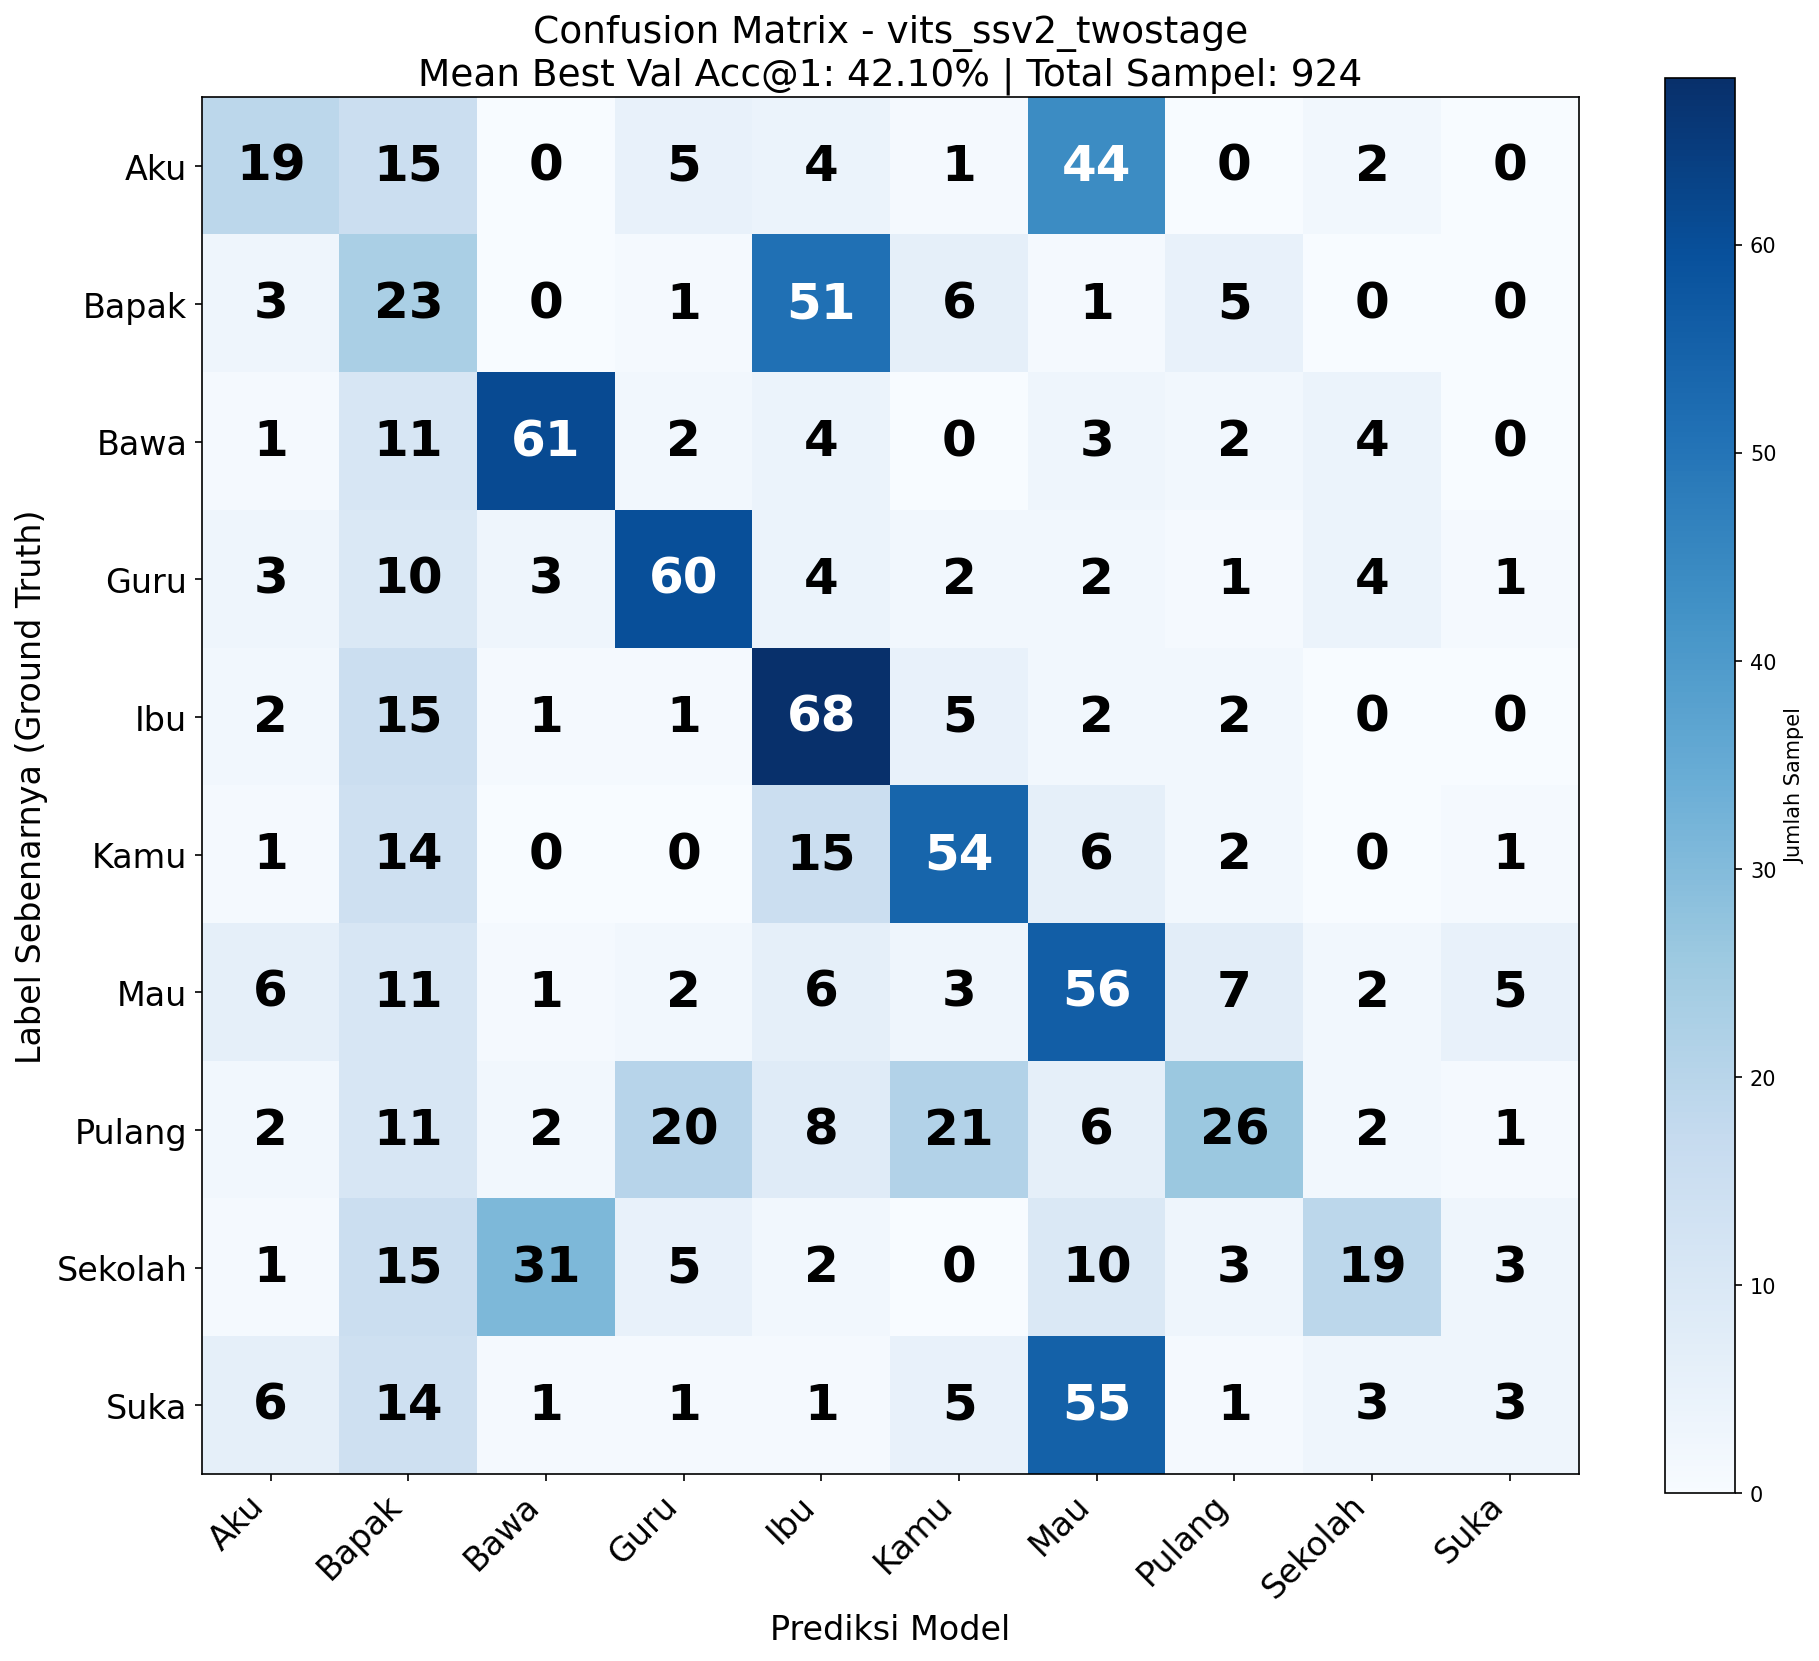
\includegraphics[width=0.95\textwidth]{figure/cm_vits_ssv2_twostage_new_font.png}
\caption{\textit{Confusion matrix} gabungan semua fold eksperimen E5 (\textit{Two-Stage Pre-train})}
\label{fig:4.cm_e5}
\end{figure}

\textit{Confusion matrix} E5 pada Gambar~\ref{fig:4.cm_e5} menunjukkan perbedaan mencolok dibandingkan E3: diagonal utama jauh lebih dominan dengan intensitas yang tinggi, mencerminkan peningkatan akurasi yang substansial. Sebagian besar kelas dapat diprediksi dengan benar pada proporsi yang cukup tinggi, terutama \textit{Bawa}, \textit{Guru}, \textit{Ibu}, dan \textit{Aku}. Kesalahan terbesar terjadi pada kelas \textit{Suka}, di mana sejumlah besar sampel diprediksi sebagai kelas lain, serta pada \textit{Sekolah} dan \textit{Pulang} yang menunjukkan distribusi prediksi yang lebih menyebar. Kelas \textit{Bapak} memiliki presisi tinggi namun beberapa sampelnya salah diprediksi sebagai \textit{Mau} atau \textit{Ibu}, yang mengindikasikan adanya kemiripan pola gerakan antara ketiga gestur ini. Secara keseluruhan, perubahan dramatis dari matriks E3 ke E5 memvisualisasikan dengan jelas dampak besar dari strategi \textit{two-stage pre-train} dalam meningkatkan kemampuan diskriminasi model.\par

Berdasarkan seluruh hasil pada bagian ini, strategi E5 (\textit{two-stage pre-train}) terbukti jauh unggul dan ditetapkan sebagai pendekatan pelatihan yang digunakan pada eksperimen selanjutnya.\par

%===========================================================================
\subsection{Pengaruh Jumlah \textit{Epoch} \textit{Stage} 2 terhadap Performa Model} \label{IV.Sek4}
%===========================================================================

Bagian ini menganalisis pengaruh durasi pelatihan pada \textit{stage} 2 terhadap performa model \textit{two-stage pre-train} menggunakan \textit{backbone} ViT-Small dengan bobot SSV2. Tiga konfigurasi jumlah epoch diuji (10, 50, dan 100 epoch), sedangkan \textit{stage} 1 dan seluruh parameter lainnya ditetapkan identik. Konfigurasi 50 epoch yang diuji dalam bagian ini identik dengan E5 dari Bagian~\ref{IV.Sek2}, sehingga kode E5 tetap digunakan sebagai titik referensi perbandingan. Konfigurasi lengkap disajikan pada Tabel~\ref{tab:4.s3_config}.\par

\begin{table}[H]
\centering
\caption{Konfigurasi eksperimen analisis jumlah \textit{epoch} \textit{stage} 2}
\label{tab:4.s3_config}
{\setlength{\tabcolsep}{3pt}
\footnotesize
\begin{tabular}{|l|l|l|l|}
\hline
\rowcolor{gray!15} \multicolumn{1}{|c|}{\textbf{Parameter}} & \multicolumn{1}{c|}{\textbf{E8}} & \multicolumn{1}{c|}{\textbf{E5}} & \multicolumn{1}{c|}{\textbf{E9}} \\
\hline
Strategi Pelatihan & \multicolumn{3}{l|}{\textit{Two-Stage Pre-train}} \\
\hline
Inisialisasi & \multicolumn{3}{l|}{Bobot SSV2} \\
\hline
\textit{Epoch Stage} 1 & \multicolumn{1}{r|}{5} & \multicolumn{1}{r|}{5} & \multicolumn{1}{r|}{5} \\
\hline
\textit{Epoch Stage} 2 & \multicolumn{1}{r|}{10} & \multicolumn{1}{r|}{50} & \multicolumn{1}{r|}{100} \\
\hline
\textit{Learning Rate Stage} 1 & \multicolumn{1}{r|}{$10^{-3}$} & \multicolumn{1}{r|}{$10^{-3}$} & \multicolumn{1}{r|}{$10^{-3}$} \\
\hline
\textit{Learning Rate Stage} 2 & \multicolumn{1}{r|}{$10^{-5}$} & \multicolumn{1}{r|}{$10^{-5}$} & \multicolumn{1}{r|}{$10^{-5}$} \\
\hline
\textit{Batch Size} & \multicolumn{1}{r|}{16} & \multicolumn{1}{r|}{16} & \multicolumn{1}{r|}{16} \\
\hline
\textit{Hyperparameter} Lain & \multicolumn{3}{l|}{Sama dengan Tabel~\ref{tab:4.umum_config}} \\
\hline
\end{tabular}
}
\end{table}

\begin{table}[H]
\centering
\caption{Nilai \textit{Best Val Acc@1} (\%) per fold dan ringkasan hasil eksperimen E8, E5, dan E9}
\label{tab:4.s3_fold}
{\setlength{\tabcolsep}{3pt}
\footnotesize
\begin{tabular}{|l|r|r|r|r|r|r|r|}
\hline
\rowcolor{gray!15} \multicolumn{1}{|c|}{Kode} & \multicolumn{1}{c|}{Fold 1} & \multicolumn{1}{c|}{Fold 2} & \multicolumn{1}{c|}{Fold 3} & \multicolumn{1}{c|}{Fold 4} & \multicolumn{1}{c|}{Fold 5} & \multicolumn{1}{c|}{\makecell[c]{Rata-\\rata}} & \multicolumn{1}{c|}{Terbaik} \\
\hline
\rowcolor{highlightpink}E8  & 54.59 & 62.50 & 57.84 & 66.49 & 60.00 & 60.28 & 66.49 \\
\hline
E5  & 62.16 & 63.59 & 62.16 & 70.27 & 61.08 & 63.85 & 70.27 \\
\hline
\rowcolor{highlightgreen}E9 & 65.41 & 66.30 & 64.32 & 70.81 & 65.95 & 66.56 & 70.81 \\
\hline
\end{tabular}
}
\end{table}

Tabel~\ref{tab:4.s3_fold} menunjukkan tren peningkatan yang konsisten seiring bertambahnya jumlah epoch pada \textit{stage} 2. Konfigurasi E8 (10 epoch) menghasilkan rata-rata akurasi 60.28\%, meningkat menjadi 63.85\% pada E5 (50 epoch), dan mencapai 66.56\% pada E9 (100 epoch). Peningkatan sebesar 6.28 poin persentase dari E8 ke E9 mengindikasikan bahwa model masih berada dalam fase peningkatan aktif dan belum mencapai titik kejenuhan dalam rentang epoch yang diuji. Yang menarik adalah Fold 4 secara konsisten menghasilkan nilai tertinggi di semua konfigurasi (66.49\%, 70.27\%, dan 70.81\%), mengindikasikan bahwa distribusi data validasi pada fold ini lebih mudah dikenali dibandingkan fold lainnya. Perbedaan antar fold yang cukup besar pada E8 (54.59\%--66.49\%) menyempit pada E9 (64.32\%--70.81\%), menunjukkan bahwa epoch yang lebih banyak tidak hanya meningkatkan rata-rata akurasi tetapi juga menghasilkan performa yang lebih konsisten antar fold.\par
Tabel~\ref{tab:4.s3_fold} menunjukkan tren peningkatan yang konsisten seiring bertambahnya jumlah epoch pada \textit{stage} 2. Konfigurasi E8 (10 epoch) menghasilkan rata-rata akurasi 60.28\%, meningkat menjadi 63.85\% pada E5 (50 epoch), dan mencapai 66.56\% pada E9 (100 epoch). Peningkatan sebesar 6.28 poin persentase dari E8 ke E9 mengindikasikan bahwa model masih berada dalam fase peningkatan aktif dan belum mencapai titik kejenuhan dalam rentang epoch yang diuji. Yang menarik adalah Fold 4 secara konsisten menghasilkan nilai tertinggi di semua konfigurasi (66.49\%, 70.27\%, dan 70.81\%), mengindikasikan bahwa distribusi data validasi pada fold ini lebih mudah dikenali dibandingkan fold lainnya. Perbedaan antar fold yang cukup besar pada E8 (54.59\%--66.49\%) menyempit pada E9 (64.32\%--70.81\%), menunjukkan bahwa epoch yang lebih banyak tidak hanya meningkatkan rata-rata akurasi tetapi juga menghasilkan performa yang lebih konsisten antarfold.\par

Gambar~\ref{fig:4.lc_e8} dan Gambar~\ref{fig:4.lc_e9} menampilkan kurva pelatihan rata-rata untuk E8 (10 epoch) dan E9 (100 epoch), sedangkan kurva E5 (50 epoch) telah ditampilkan pada Gambar~\ref{fig:4.lc_e5} (Bagian~\ref{IV.Sek2}).\par

\begin{figure}[H]
\centering
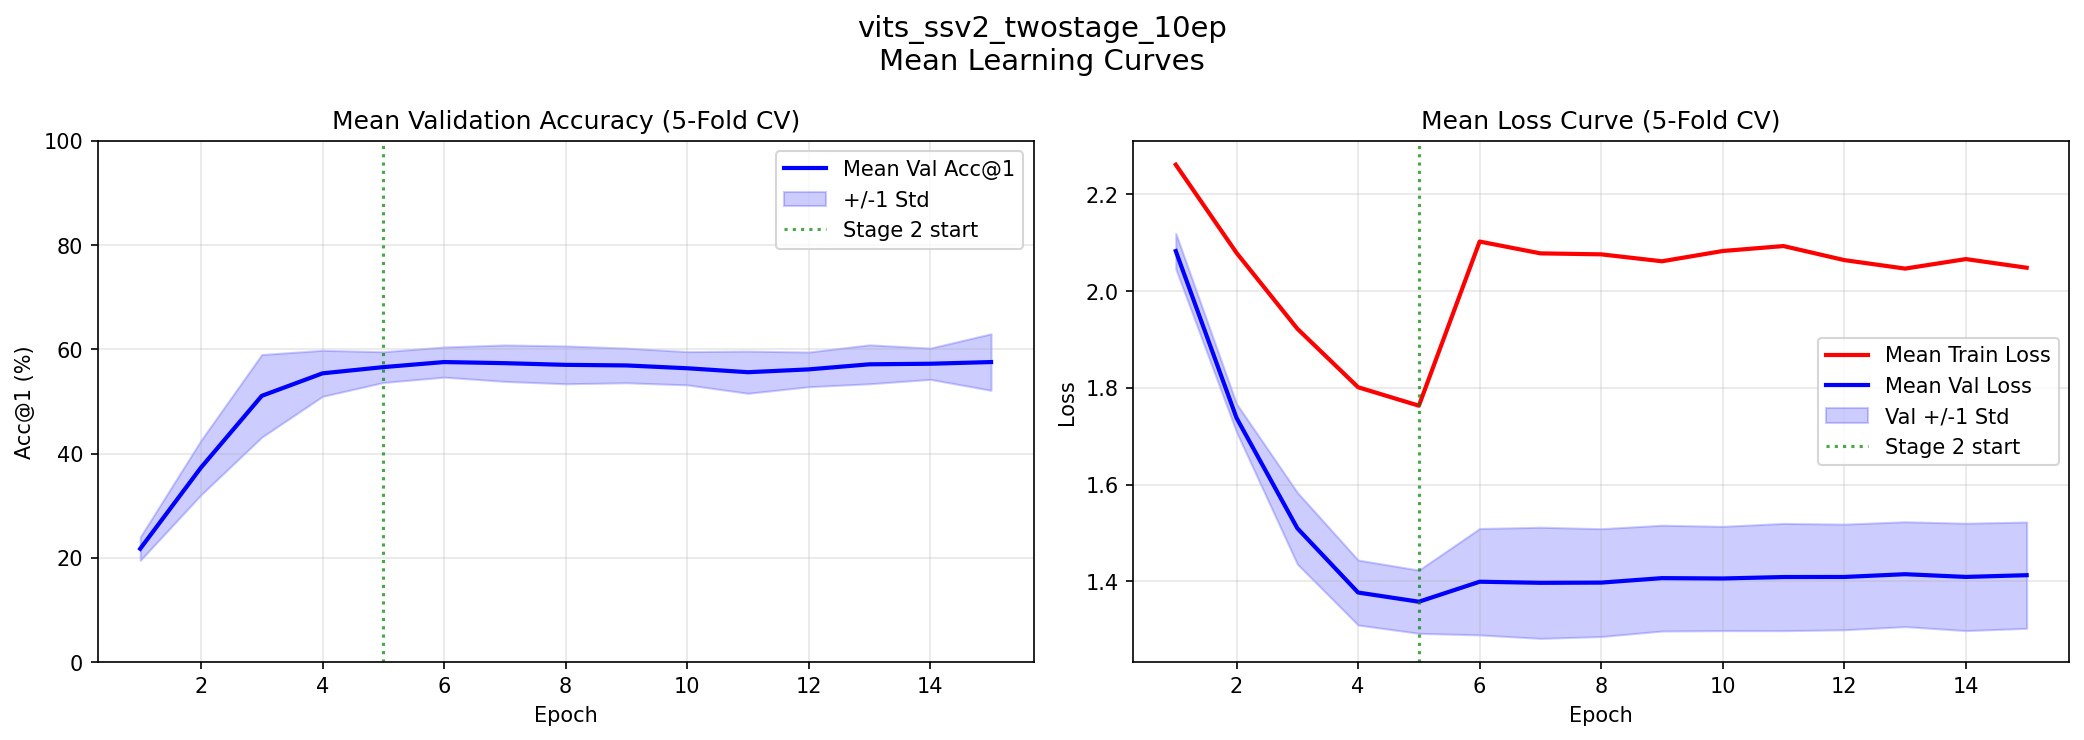
\includegraphics[width=0.95\textwidth]{figure/lc_vits_ssv2_twostage_10ep.png}
\caption{Kurva pelatihan rata-rata eksperimen E8 (\textit{Stage} 2 = 10 epoch)}
\label{fig:4.lc_e8}
\end{figure}

Kurva E8 pada Gambar~\ref{fig:4.lc_e8} memperlihatkan bahwa model masih dalam fase peningkatan aktif ketika pelatihan dihentikan pada epoch ke-10. Akurasi validasi cenderung masih meningkat di akhir \textit{stage} 2 tanpa menunjukkan tanda-tanda melandai, yang secara jelas mengindikasikan kondisi \textit{underfitting}, model belum memiliki cukup waktu pelatihan untuk mengekstraksi seluruh pola diskriminatif yang tersedia dalam data. Variabilitas antar fold juga lebih tinggi dibandingkan E5 dan E9, yang merupakan konsekuensi dari durasi pelatihan yang terlalu singkat sehingga model sensitif terhadap variasi distribusi data pada setiap fold. Meskipun demikian, capaian 60.28\% dengan hanya 10 epoch sudah jauh melampaui E3 (35.18\%), kembali membuktikan besarnya kontribusi bobot \textit{pre-train} SSV2 dalam mempercepat konvergensi. Sebagai perbandingan, kurva E5 (50 epoch) pada Gambar~\ref{fig:4.lc_e5} menunjukkan konvergensi yang lebih penuh, dengan akurasi validasi yang mulai melandai pada sekitar epoch ke-30 hingga ke-40, mengindikasikan bahwa 50 epoch sudah mencukupi untuk sebagian besar proses pembelajaran meskipun peningkatan lebih lanjut masih dimungkinkan.\par
Kurva E8 pada Gambar~\ref{fig:4.lc_e8} memperlihatkan bahwa model masih dalam fase peningkatan aktif ketika pelatihan dihentikan pada epoch ke-10. Akurasi validasi cenderung masih meningkat di akhir \textit{stage} 2 tanpa menunjukkan tanda-tanda melandai, yang secara jelas mengindikasikan kondisi \textit{underfitting}, model belum memiliki cukup waktu pelatihan untuk mengekstraksi seluruh pola diskriminatif yang tersedia dalam data. Variabilitas antarfold juga lebih tinggi dibandingkan E5 dan E9, yang merupakan konsekuensi dari durasi pelatihan yang terlalu singkat sehingga model sensitif terhadap variasi distribusi data pada setiap fold. Meskipun demikian, capaian 60.28\% dengan hanya 10 epoch sudah jauh melampaui E3 (35.18\%), kembali membuktikan besarnya kontribusi bobot \textit{pre-train} SSV2 dalam mempercepat konvergensi. Sebagai perbandingan, kurva E5 (50 epoch) pada Gambar~\ref{fig:4.lc_e5} menunjukkan konvergensi yang lebih penuh, dengan akurasi validasi yang mulai melandai pada sekitar epoch ke-30 hingga ke-40, mengindikasikan bahwa 50 epoch sudah mencukupi untuk sebagian besar proses pembelajaran meskipun peningkatan lebih lanjut masih dimungkinkan.\par

\begin{figure}[H]
\centering
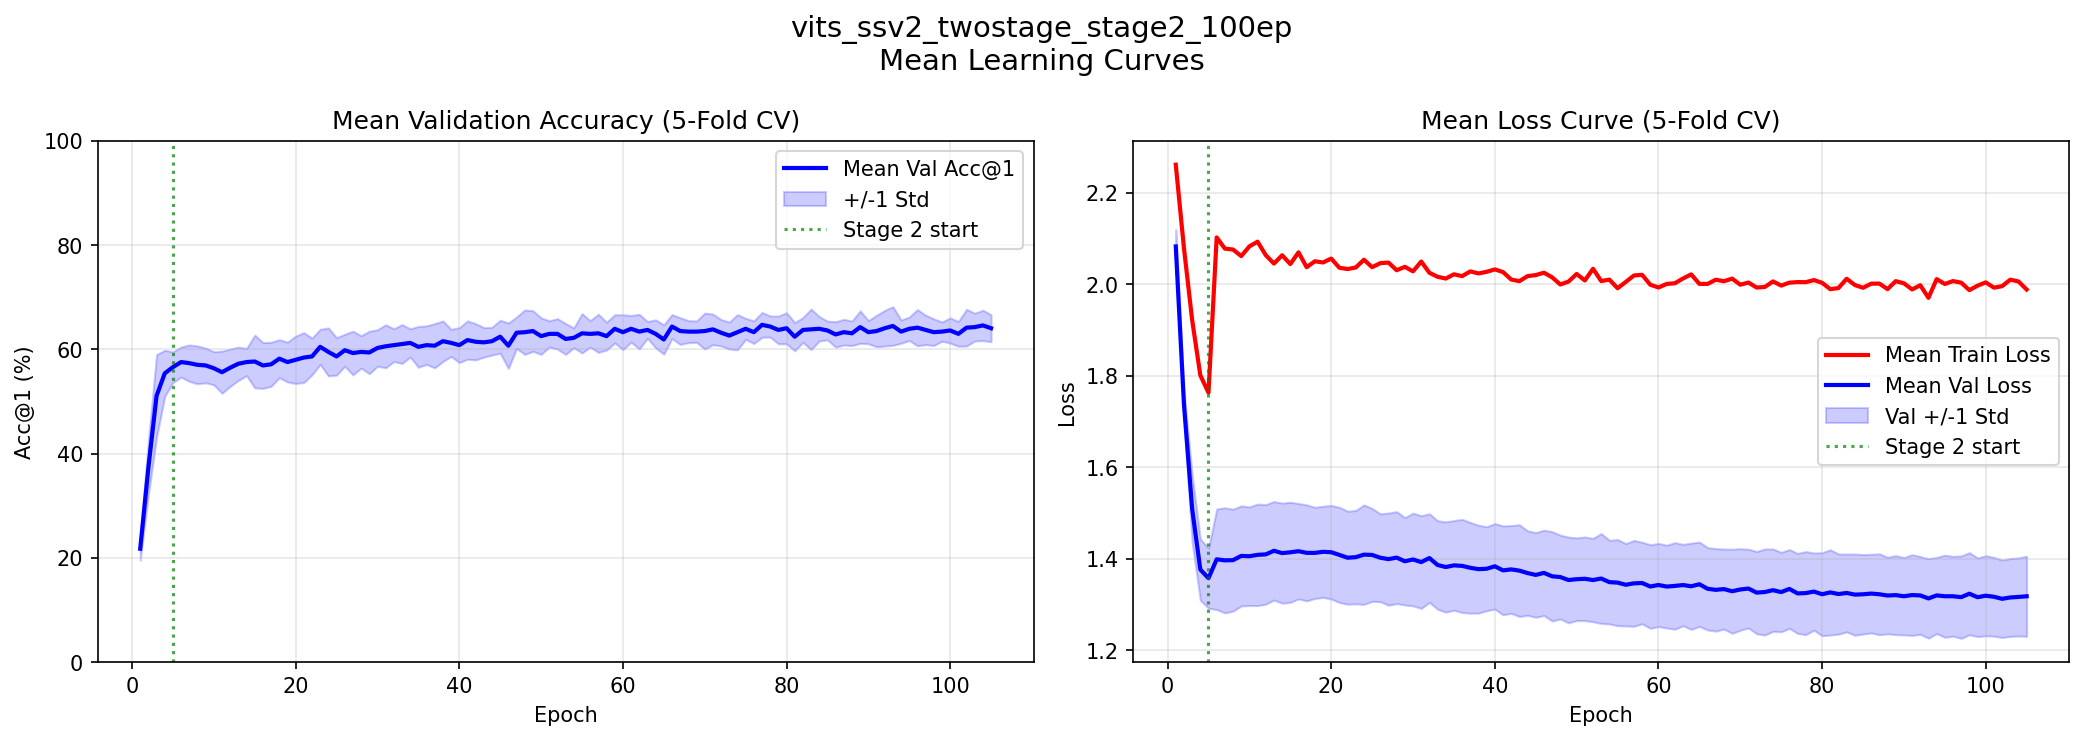
\includegraphics[width=0.95\textwidth]{figure/lc_vits_ssv2_twostage_stage2_100ep.png}
\caption{Kurva pelatihan rata-rata eksperimen E9 (\textit{Stage} 2 = 100 epoch)}
\label{fig:4.lc_e9}
\end{figure}

Kurva E9 pada Gambar~\ref{fig:4.lc_e9} memperlihatkan bahwa model masih mengalami peningkatan moderat bahkan di epoch-epoch akhir mendekati epoch ke-100, mengindikasikan bahwa model belum sepenuhnya jenuh dan masih ada ruang untuk peningkatan jika durasi pelatihan diperpanjang lebih lanjut. Tren akurasi validasi pada E9 lebih mulus dibandingkan E5, kemungkinan karena \textit{learning rate} yang sangat kecil ($10^{-5}$) menghasilkan pembaruan parameter yang lebih halus dan stabil. Tidak ditemukan divergensi antara \textit{training} dan \textit{validation accuracy} yang merupakan tanda klasik \textit{overfitting}, mengonfirmasi bahwa regularisasi yang diterapkan cukup efektif pada rentang 100 epoch ini.\par

Tabel~\ref{tab:4.s3_perkelas} menyajikan perbandingan laporan klasifikasi per kelas gabungan seluruh fold untuk ketiga konfigurasi epoch.\par

\begin{table}[H]
\centering
\caption{Laporan klasifikasi per kelas (gabungan semua fold): E8, E5, dan E9}
\label{tab:4.s3_perkelas}
{\setlength{\tabcolsep}{3pt}
\footnotesize
\begin{tabular}{|l|rrr|rrr|rrr|}
\hline
\rowcolor{gray!15} \multicolumn{1}{|c|}{\multirow{2}{*}{\textbf{Kelas}}} & \multicolumn{3}{c|}{\cellcolor{gray!15}\textbf{E8 (10 epoch)}} & \multicolumn{3}{c|}{\cellcolor{gray!15}\textbf{E5 (50 epoch)}} & \multicolumn{3}{c|}{\cellcolor{gray!15}\textbf{E9 (100 epoch)}} \\
\cline{2-10}
 & \multicolumn{1}{c|}{$P$} & \multicolumn{1}{c|}{$R$} & \multicolumn{1}{c|}{$F_1$} & \multicolumn{1}{c|}{$P$} & \multicolumn{1}{c|}{$R$} & \multicolumn{1}{c|}{$F_1$} & \multicolumn{1}{c|}{$P$} & \multicolumn{1}{c|}{$R$} & \multicolumn{1}{c|}{$F_1$} \\
\hline
Aku     & 0.52 & 0.64 & 0.58 & 0.66 & 0.70 & 0.68 & 0.74 & 0.72 & 0.73 \\
Bapak   & 0.65 & 0.62 & 0.64 & 0.81 & 0.52 & 0.64 & 0.90 & 0.50 & 0.64 \\
Bawa    & 0.62 & 0.99 & 0.76 & 0.62 & 1.00 & 0.76 & 0.65 & 1.00 & 0.79 \\
Guru    & 0.77 & 0.80 & 0.79 & 0.79 & 0.84 & 0.82 & 0.79 & 0.91 & 0.85 \\
Ibu     & 0.47 & 0.74 & 0.57 & 0.54 & 0.86 & 0.66 & 0.57 & 0.91 & 0.70 \\
Kamu    & 0.54 & 0.45 & 0.49 & 0.60 & 0.60 & 0.60 & 0.68 & 0.70 & 0.69 \\
Mau     & 0.42 & 0.61 & 0.50 & 0.43 & 0.68 & 0.52 & 0.51 & 0.67 & 0.58 \\
Pulang  & 0.63 & 0.32 & 0.43 & 0.69 & 0.38 & 0.49 & 0.75 & 0.51 & 0.60 \\
Sekolah & 0.73 & 0.30 & 0.43 & 0.82 & 0.35 & 0.49 & 0.86 & 0.42 & 0.56 \\
Suka    & 0.42 & 0.16 & 0.23 & 0.58 & 0.21 & 0.31 & 0.67 & 0.43 & 0.53 \\
\hline
\textit{Macro} Avg & 0.58 & 0.56 & 0.54 & 0.65 & 0.61 & 0.60 & 0.71 & 0.68 & 0.67 \\
\hline
\end{tabular}
}
\end{table}

Tabel~\ref{tab:4.s3_perkelas} memperlihatkan bahwa peningkatan epoch secara konsisten memperbaiki metrik di hampir seluruh kelas. Kelas yang paling signifikan meningkat dari E8 ke E9 adalah \textit{Suka} (F1: 0.23 $\rightarrow$ 0.53), \textit{Pulang} (0.43 $\rightarrow$ 0.60), dan \textit{Kamu} (0.49 $\rightarrow$ 0.69), ketiga kelas ini merupakan kelas yang relatif sulit pada eksperimen-eksperimen sebelumnya, dan hasilnya menunjukkan bahwa epoch yang lebih banyak memungkinkan model untuk mempelajari pola diskriminatif yang lebih halus dari gestur-gestur tersebut. Kelas \textit{Bawa} mempertahankan \textit{recall} sempurna (1.00) di seluruh konfigurasi, mengonfirmasi bahwa gestur ini memiliki karakteristik visual yang sangat kuat sehingga mudah dipelajari bahkan dengan durasi pelatihan yang singkat. Kelas \textit{Bapak} menunjukkan pola yang menarik, presisinya terus meningkat (0.65 $\rightarrow$ 0.90) namun \textit{recall}-nya menurun (0.62 $\rightarrow$ 0.50) seiring bertambahnya epoch, mengindikasikan bahwa model menjadi semakin selektif dalam memprediksi kelas ini, hanya memprediksi ``Bapak'' pada kasus yang sangat jelas sehingga beberapa sampel yang ambigu diabaikan. Nilai \textit{Macro} F1 yang meningkat secara konsisten (0.54 $\rightarrow$ 0.60 $\rightarrow$ 0.67) menegaskan bahwa peningkatan epoch bermanfaat secara merata di seluruh kelas, bukan hanya pada kelas tertentu.\par

Gambar~\ref{fig:4.cm_e9} menampilkan \textit{confusion matrix} gabungan seluruh fold untuk eksperimen E9 yang merupakan konfigurasi terbaik.\par

\begin{figure}[H]
\centering
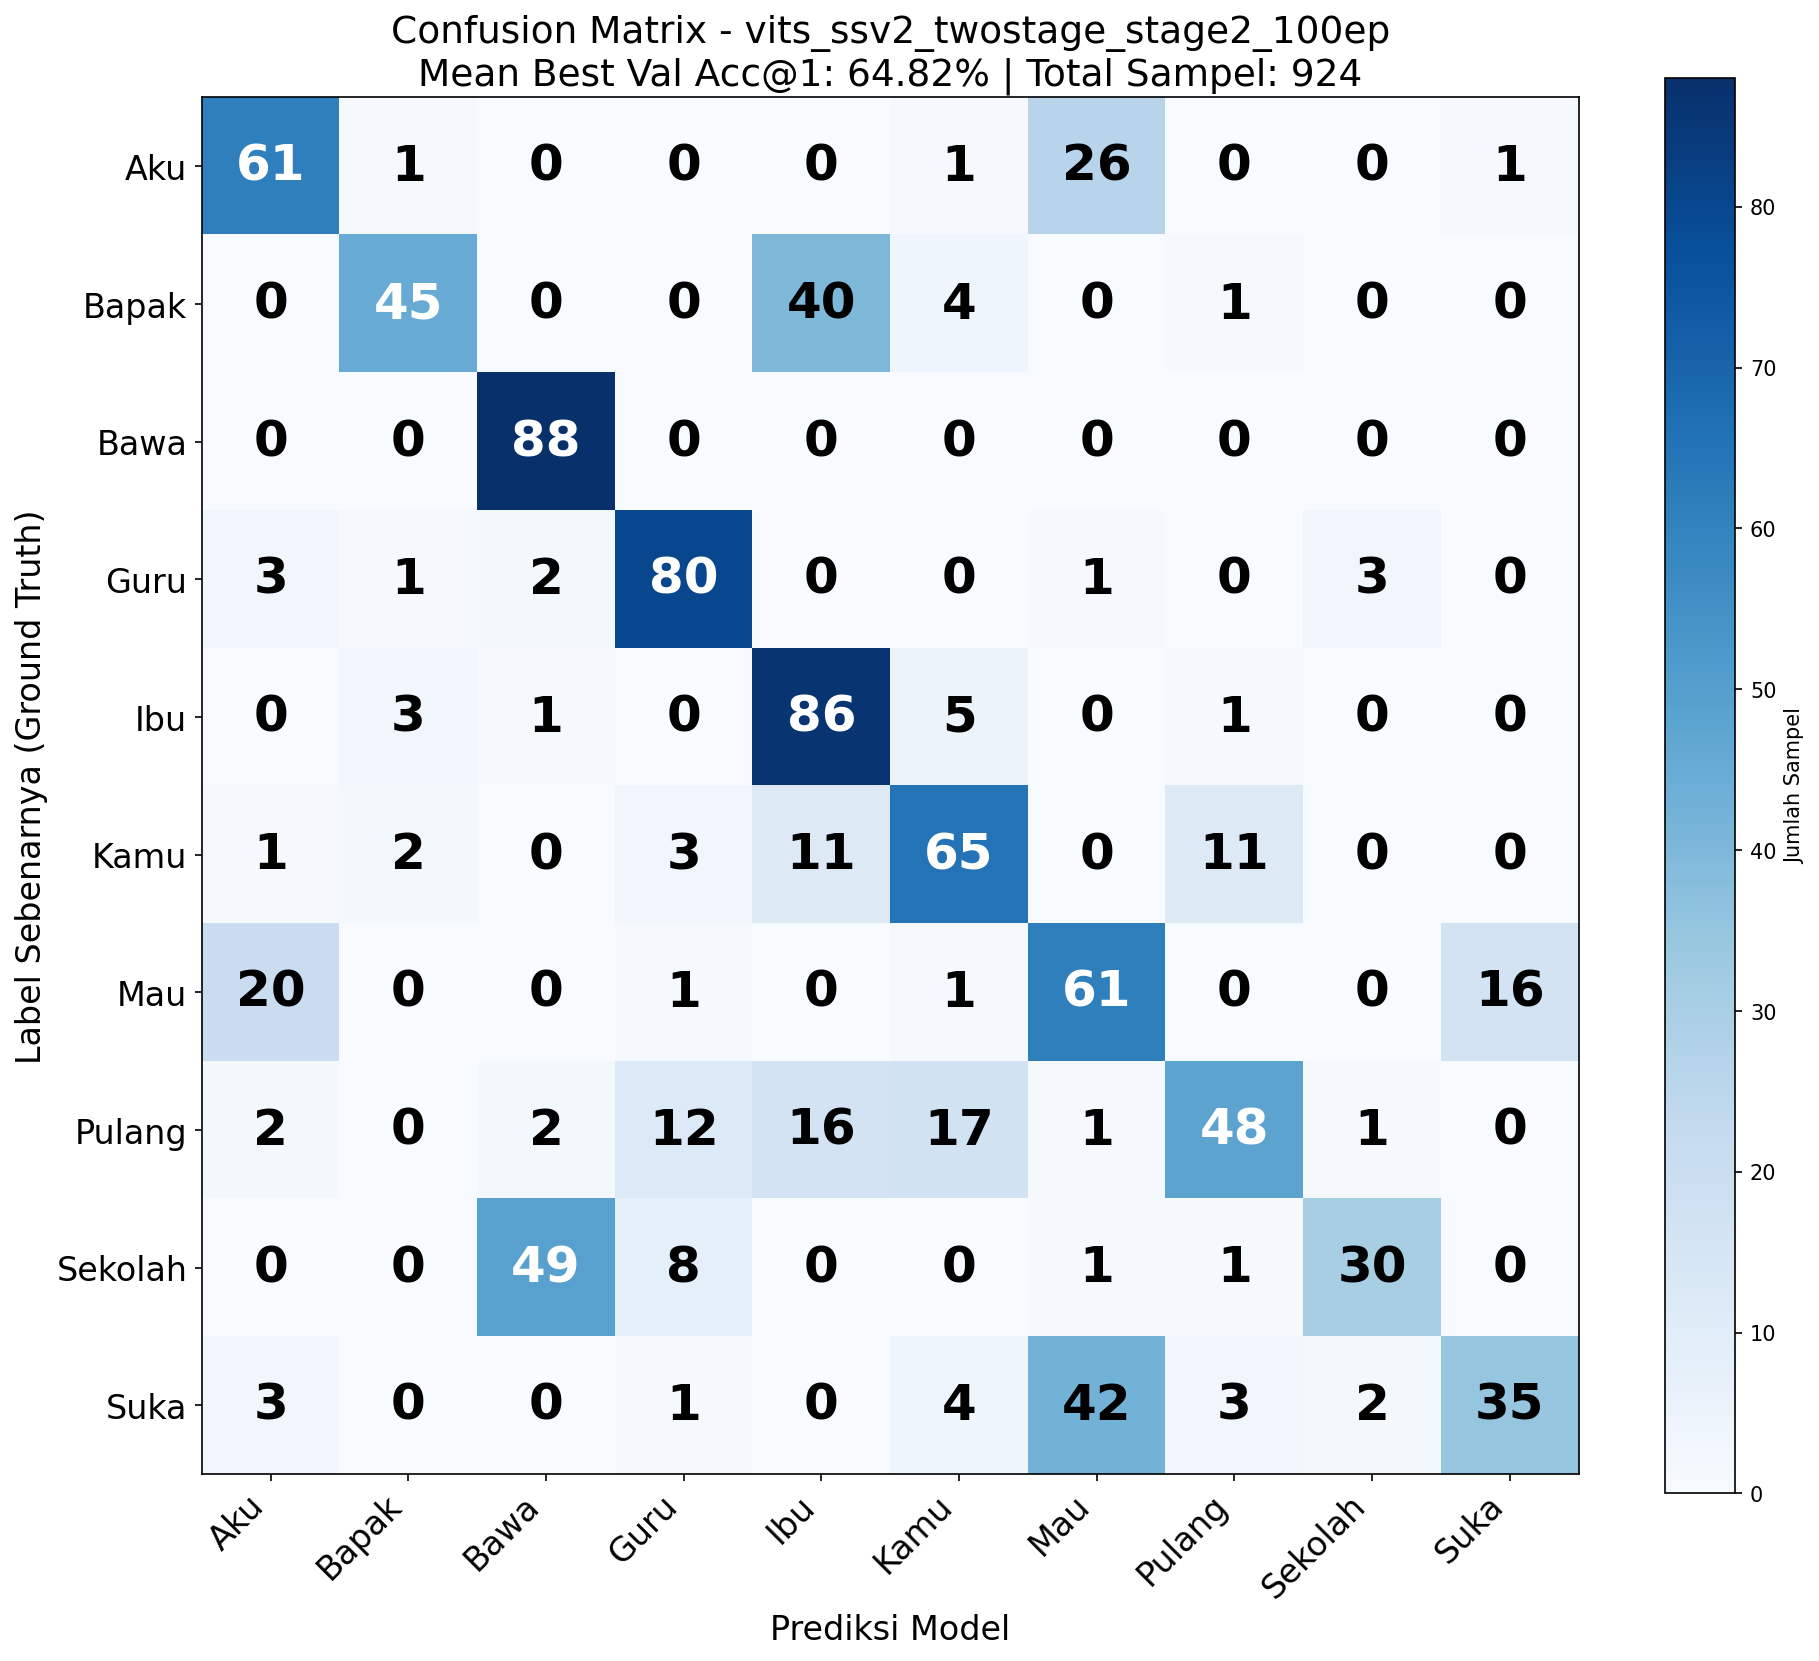
\includegraphics[width=0.95\textwidth]{figure/cm_vits_ssv2_twostage_stage2_100ep_new_font.png}
\caption{\textit{Confusion matrix} gabungan semua fold eksperimen E9 (\textit{Stage} 2 = 100 epoch)}
\label{fig:4.cm_e9}
\end{figure}

\textit{Confusion matrix} E9 pada Gambar~\ref{fig:4.cm_e9} menampilkan diagonal yang lebih dominan dibandingkan matriks E5 (Gambar~\ref{fig:4.cm_e5}), mencerminkan peningkatan kemampuan klasifikasi yang dicapai dengan tambahan epoch pelatihan. Sel-sel di luar diagonal tampak lebih pudar secara keseluruhan, mengindikasikan berkurangnya kesalahan prediksi antar kelas secara umum. Kelas \textit{Bawa}, \textit{Guru}, dan \textit{Ibu} menunjukkan nilai diagonal yang paling menonjol, sesuai dengan F1-\textit{score} tertinggi mereka pada Tabel~\ref{tab:4.s3_perkelas}. Beberapa pola kesalahan yang persisten masih terlihat, terutama pada kelas \textit{Suka} yang sebagian sampelnya masih terprediksi sebagai \textit{Mau} atau \textit{Kamu}, serta kelas \textit{Sekolah} yang masih memiliki distribusi kesalahan yang cukup menyebar. Meski demikian, matriks ini secara visual mengonfirmasi bahwa E9 merupakan konfigurasi dengan kemampuan diskriminasi terbaik di antara seluruh skenario epoch yang diuji.\par
\textit{Confusion matrix} E9 pada Gambar~\ref{fig:4.cm_e9} menampilkan diagonal yang lebih dominan dibandingkan matriks E5 (Gambar~\ref{fig:4.cm_e5}), mencerminkan peningkatan kemampuan klasifikasi yang dicapai dengan tambahan epoch pelatihan. Sel-sel di luar diagonal tampak lebih pudar secara keseluruhan, mengindikasikan berkurangnya kesalahan prediksi antarkelas secara umum. Kelas \textit{Bawa}, \textit{Guru}, dan \textit{Ibu} menunjukkan nilai diagonal yang paling menonjol, sesuai dengan F1-\textit{score} tertinggi mereka pada Tabel~\ref{tab:4.s3_perkelas}. Beberapa pola kesalahan yang persisten masih terlihat, terutama pada kelas \textit{Suka} yang sebagian sampelnya masih terprediksi sebagai \textit{Mau} atau \textit{Kamu}, serta kelas \textit{Sekolah} yang masih memiliki distribusi kesalahan yang cukup menyebar. Meski demikian, matriks ini secara visual mengonfirmasi bahwa E9 merupakan konfigurasi dengan kemampuan diskriminasi terbaik di antara seluruh skenario epoch yang diuji.\par
%===========================================================================
\subsection{Perbandingan Strategi \textit{Sampling} Frame \textit{Dense} dan \textit{Uniform}} \label{IV.Sek3}
%===========================================================================

Bagian ini menganalisis pengaruh strategi \textit{sampling} frame terhadap performa model dengan membandingkan \textit{dense sampling} dan \textit{uniform sampling} pada konfigurasi \textit{two-stage pre-train} ViT-Small + SSV2 dengan \textit{stage} 2 sebanyak 50 epoch. \textit{Dense sampling} mengambil 16 frame secara berurutan dari segmen video yang rapat, sehingga menangkap informasi temporal lokal yang halus namun berisiko hanya merepresentasikan sebagian durasi gestur. \textit{Uniform sampling} mengambil 16 frame secara merata di sepanjang keseluruhan durasi video, memastikan seluruh fase gestur, dari posisi awal tangan, fase gerak inti, hingga posisi akhir, terwakili dalam satu klip masukan. Seluruh parameter pelatihan identik antara kedua eksperimen. Konfigurasi disajikan pada Tabel~\ref{tab:4.s4_config}.\par

\begin{table}[H]
\centering
\caption{Konfigurasi eksperimen perbandingan strategi \textit{sampling}}
\label{tab:4.s4_config}
{\setlength{\tabcolsep}{3pt}
\footnotesize
\begin{tabular}{|l|p{2.8cm}|p{2.8cm}|}
\hline
\rowcolor{gray!15} \multicolumn{1}{|c|}{\textbf{Parameter}} & \multicolumn{1}{c|}{\textbf{E5}} & \multicolumn{1}{c|}{\textbf{E10}} \\
\hline
Strategi \textit{Sampling} & \textit{Uniform} & \textit{Dense} \\
\hline
\textit{Epoch Stage} 1 & \multicolumn{1}{r|}{5} & \multicolumn{1}{r|}{5} \\
\hline
\textit{Epoch Stage} 2 & \multicolumn{1}{r|}{50} & \multicolumn{1}{r|}{50} \\
\hline
Jumlah \textit{Frame} & \multicolumn{1}{r|}{16} & \multicolumn{1}{r|}{16} \\
\hline
\textit{Batch Size} & \multicolumn{1}{r|}{16} & \multicolumn{1}{r|}{16} \\
\hline
\textit{Learning Rate} & \multicolumn{1}{r|}{$10^{-3}$} & \multicolumn{1}{r|}{$10^{-3}$} \\
\hline
\textit{Hyperparameter} Lain & \multicolumn{2}{l|}{Sama dengan Tabel~\ref{tab:4.umum_config}} \\
\hline
\end{tabular}
}
\end{table}

\begin{table}[H]
\centering
\caption{Nilai \textit{Best Val Acc@1} (\%) per fold dan ringkasan hasil eksperimen E5 dan E10}
\label{tab:4.s4_fold}
{\setlength{\tabcolsep}{3pt}
\footnotesize
\begin{tabular}{|l|r|r|r|r|r|r|r|}
\hline
\rowcolor{gray!15} \multicolumn{1}{|c|}{Kode} & \multicolumn{1}{c|}{Fold 1} & \multicolumn{1}{c|}{Fold 2} & \multicolumn{1}{c|}{Fold 3} & \multicolumn{1}{c|}{Fold 4} & \multicolumn{1}{c|}{Fold 5} & \multicolumn{1}{c|}{\makecell[c]{Rata-\\rata}} & \multicolumn{1}{c|}{Terbaik} \\
\hline
\rowcolor{highlightgreen}E5  & 62.16 & 63.59 & 62.16 & 70.27 & 61.08 & 63.85 & 70.27 \\
\hline
\rowcolor{highlightpink}E10 & 54.59 & 61.96 & 55.14 & 57.30 & 51.35 & 56.07 & 61.96 \\
\hline
\end{tabular}
}
\end{table}

Tabel~\ref{tab:4.s4_fold} menunjukkan bahwa penggunaan \textit{dense sampling} pada E10 menyebabkan penurunan performa dibandingkan \textit{uniform sampling} pada E5 di seluruh fold tanpa pengecualian. Rata-rata akurasi menurun sebesar 7.78 poin persentase dari 63.85\% pada E5 menjadi 56.07\% pada E10. Penurunan terbesar terjadi pada Fold 4 (70.27\% menjadi 57.30\%), sedangkan penurunan terkecil terjadi pada Fold 2 (63.59\% menjadi 61.96\%). Konsistensi penurunan performa pada seluruh fold menunjukkan bahwa strategi \textit{dense sampling} kurang sesuai dengan karakteristik temporal gestur SIBI dibandingkan \textit{uniform sampling}. Nilai terbaik juga mengalami penurunan cukup besar dari 70.27\% pada E5 menjadi 61.96\% pada E10, memperlihatkan bahwa performa maksimum model ikut terdampak ketika menggunakan \textit{dense sampling}.\par

Gambar~\ref{fig:4.lc_e10} menampilkan kurva pelatihan rata-rata untuk eksperimen E10 (\textit{dense sampling}), sedangkan kurva pelatihan E5 (\textit{uniform sampling}) telah ditampilkan pada Gambar~\ref{fig:4.lc_e5} (Bagian~\ref{IV.Sek2}).\par

\begin{figure}[H]
\centering
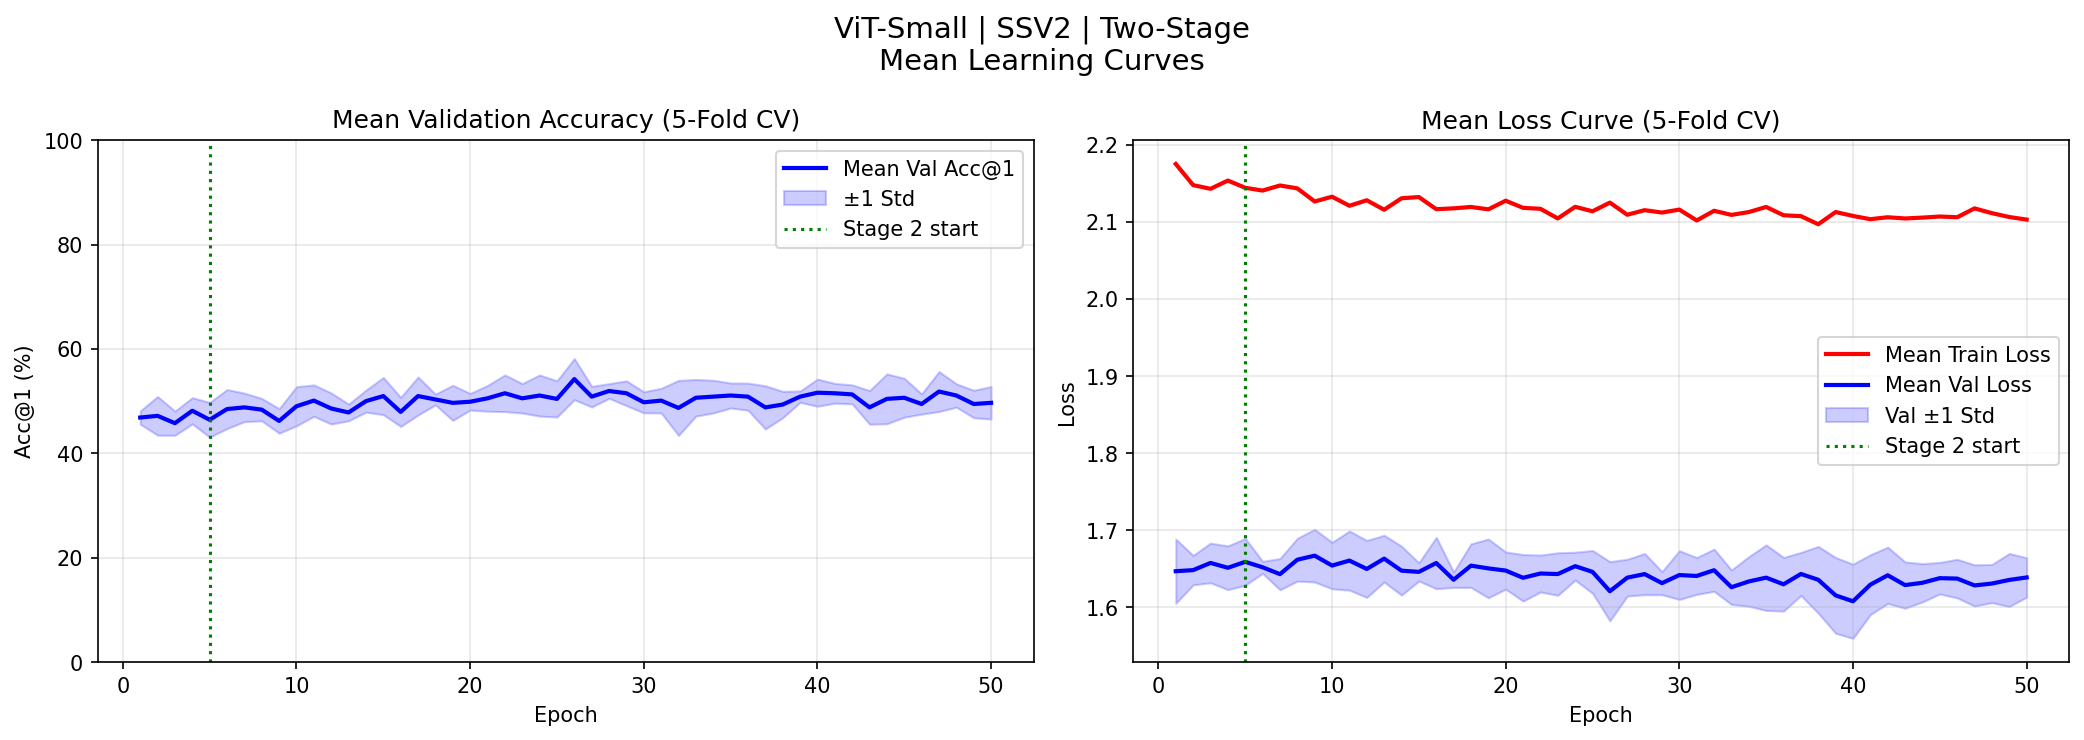
\includegraphics[width=0.95\textwidth]{figure/lc_vits_ssv2_dense.png}
\caption{Kurva pelatihan rata-rata eksperimen E10 (\textit{Dense Sampling})}
\label{fig:4.lc_e10}
\end{figure}

Kurva pelatihan E10 pada Gambar~\ref{fig:4.lc_e10} menunjukkan konvergensi yang lebih lambat dan lebih fluktuatif dibandingkan E5. Akurasi validasi bergerak dalam rentang yang lebih sempit dengan variasi antar fold yang lebih besar, mengindikasikan bahwa representasi temporal yang tidak lengkap akibat \textit{dense sampling} menyebabkan ketidakstabilan dalam proses pembelajaran. Model tampak lebih sensitif terhadap variasi fold yang kemungkinan berkaitan dengan perbedaan durasi gestur antar penutur, ketika \textit{dense sampling} menangkap segmen yang tidak representatif, kualitas pelatihan pada fold tersebut menurun secara signifikan. Meskipun kurva akhirnya mencapai nilai 56\%, laju konvergensinya lebih lambat dibandingkan E5 yang sudah mencapai nilai serupa pada epoch yang lebih awal. Sebagai perbandingan, kurva pelatihan E5 (\textit{uniform sampling}) yang ditampilkan pada Gambar~\ref{fig:4.lc_e5} memperlihatkan konvergensi yang lebih cepat, lebih stabil, dan dengan variasi antar fold yang lebih kecil, mencerminkan manfaat representasi temporal yang komprehensif dari \textit{uniform sampling}.\par

Tabel~\ref{tab:4.s4_perkelas} menyajikan perbandingan laporan klasifikasi per kelas antara E5 dan E10.\par

\begin{table}[H]
\centering
\caption{Laporan klasifikasi per kelas (gabungan semua fold): E5 dan E10}
\label{tab:4.s4_perkelas}
{\setlength{\tabcolsep}{3pt}
\footnotesize
\begin{tabular}{|l|>{\centering\arraybackslash}p{0.9cm}|>{\centering\arraybackslash}p{0.9cm}|>{\centering\arraybackslash}p{0.9cm}|>{\centering\arraybackslash}p{0.9cm}|>{\centering\arraybackslash}p{0.9cm}|>{\centering\arraybackslash}p{0.9cm}|}
\hline
\rowcolor{gray!15} \multicolumn{1}{|c|}{\multirow{2}{*}{\textbf{Kelas}}} & \multicolumn{3}{c|}{\cellcolor{gray!15}\textbf{E5 (\textit{Uniform Sampling})}} & \multicolumn{3}{c|}{\cellcolor{gray!15}\textbf{E10 (\textit{Dense Sampling})}} \\
\cline{2-7}
 & \multicolumn{1}{c|}{$P$} & \multicolumn{1}{c|}{$R$} & \multicolumn{1}{c|}{$F_1$} & \multicolumn{1}{c|}{$P$} & \multicolumn{1}{c|}{$R$} & \multicolumn{1}{c|}{$F_1$} \\
\hline
Aku     & 0.66 & 0.70 & 0.68 & 0.78 & 0.50 & 0.61 \\
Bapak   & 0.81 & 0.52 & 0.64 & 0.51 & 0.33 & 0.40 \\
Bawa    & 0.62 & 1.00 & 0.76 & 0.74 & 0.96 & 0.83 \\
Guru    & 0.79 & 0.84 & 0.82 & 0.79 & 0.88 & 0.83 \\
Ibu     & 0.54 & 0.86 & 0.66 & 0.45 & 0.79 & 0.58 \\
Kamu    & 0.60 & 0.60 & 0.60 & 0.65 & 0.77 & 0.70 \\
Mau     & 0.43 & 0.68 & 0.52 & 0.41 & 0.87 & 0.56 \\
Pulang  & 0.69 & 0.38 & 0.49 & 0.72 & 0.27 & 0.39 \\
Sekolah & 0.82 & 0.35 & 0.49 & 0.74 & 0.40 & 0.52 \\
Suka    & 0.58 & 0.21 & 0.31 & 0.38 & 0.08 & 0.14 \\
\hline
\textit{Macro} Avg & 0.65 & 0.61 & 0.60 & 0.62 & 0.59 & 0.56 \\
\hline
\end{tabular}
}
\end{table}

Perbandingan per kelas pada Tabel~\ref{tab:4.s4_perkelas} menunjukkan bahwa penggunaan \textit{dense sampling} pada E10 menyebabkan penurunan performa pada beberapa kelas dibandingkan E5. Penurunan F1-\textit{score} paling besar terjadi pada kelas \textit{Bapak}, \textit{Suka}, dan \textit{Pulang} (masing-masing 0.64$\rightarrow$0.40, 0.31$\rightarrow$0.14, dan 0.49$\rightarrow$0.39), mengindikasikan bahwa strategi \textit{dense sampling} kurang mampu menangkap pola temporal gestur yang tersebar sepanjang durasi video. Penurunan ini menunjukkan bahwa sebagian informasi penting kemungkinan tidak terambil ketika frame difokuskan hanya pada segmen tertentu secara rapat. Kelas \textit{Kamu} justru mengalami peningkatan F1 pada E10 (0.60$\rightarrow$0.70), yang mengindikasikan bahwa ciri pembeda gestur tersebut lebih terkonsentrasi pada segmen pendek sehingga lebih mudah ditangkap oleh \textit{dense sampling}. Kelas \textit{Bawa} dan \textit{Guru} juga menunjukkan performa yang relatif serupa atau sedikit lebih baik pada E10. Namun secara keseluruhan, nilai \textit{Macro} F1 tetap mengalami penurunan dari 0.60 pada E5 menjadi 0.56 pada E10, mengonfirmasi bahwa \textit{uniform sampling} memberikan performa yang lebih stabil dan merata di seluruh kelas.\par

Gambar~\ref{fig:4.cm_e10} menampilkan \textit{confusion matrix} gabungan seluruh fold untuk E10, sedangkan \textit{confusion matrix} E5 telah ditampilkan pada Gambar~\ref{fig:4.cm_e5} (Bagian~\ref{IV.Sek2}).\par

\begin{figure}[H]
\centering
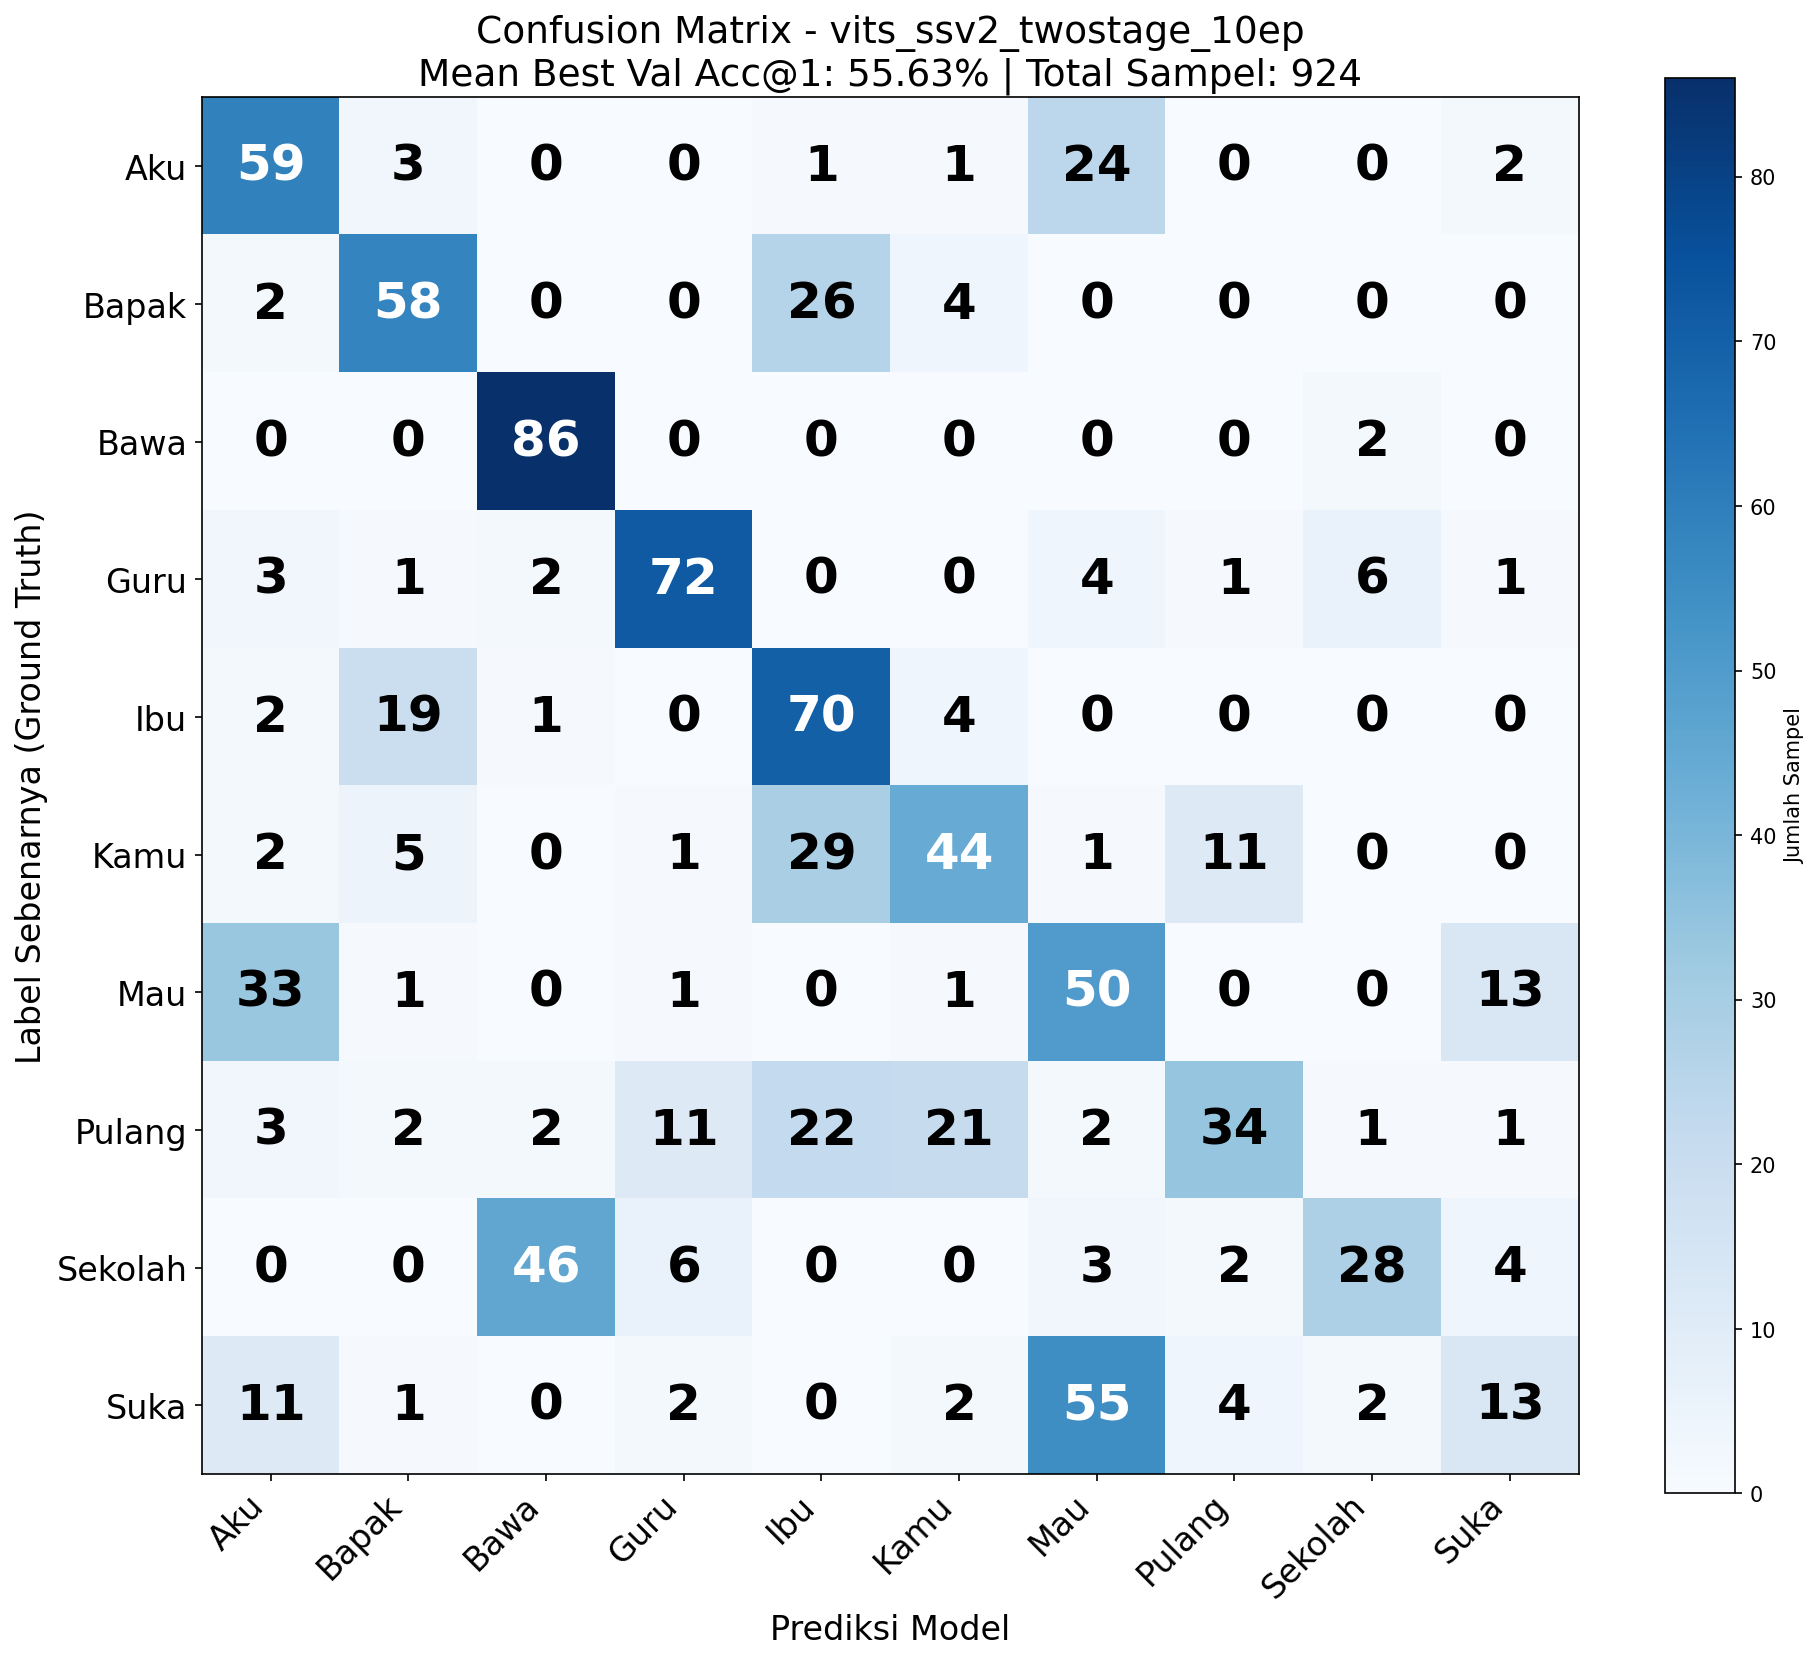
\includegraphics[width=0.95\textwidth]{figure/cm_vits_ssv2_dense_new_font.png}
\caption{\textit{Confusion matrix} gabungan semua fold eksperimen E10 (\textit{Dense Sampling})}
\label{fig:4.cm_e10}
\end{figure}

\textit{Confusion matrix} E10 pada Gambar~\ref{fig:4.cm_e10} menunjukkan pola diagonal yang kurang dominan dibandingkan E5, dengan beberapa sel di luar diagonal yang masih cukup kuat. Kelas \textit{Suka} memiliki nilai diagonal yang sangat rendah, sebagian besar sampelnya terprediksi sebagai kelas lain, terutama \textit{Mau} dan \textit{Kamu}, yang merupakan konsekuensi dari \textit{recall} yang sangat rendah (0.08). Kelas \textit{Pulang} juga menunjukkan distribusi prediksi yang menyebar luas, mengindikasikan bahwa \textit{dense sampling} gagal menangkap pola temporal khas gestur ini secara konsisten. Di sisi lain, kelas \textit{Kamu} dan \textit{Guru} memiliki diagonal yang relatif lebih kuat pada E10, konsisten dengan F1-\textit{score} keduanya yang lebih tinggi dibandingkan E5 pada kelas-kelas tersebut. Sebaliknya, \textit{confusion matrix} E5 (Gambar~\ref{fig:4.cm_e5}) menampilkan diagonal yang lebih kuat secara keseluruhan, dengan performa klasifikasi yang lebih stabil pada sebagian besar kelas, terutama \textit{Bapak}, \textit{Suka}, dan \textit{Pulang}. Hal ini kembali memperlihatkan bahwa \textit{uniform sampling} lebih efektif dalam merepresentasikan pola temporal gestur yang tersebar sepanjang durasi video.\par

Berdasarkan seluruh hasil pada bagian ini, penggunaan \textit{dense sampling} pada E10 terbukti menurunkan performa model dibandingkan \textit{uniform sampling} pada E5. Oleh karena itu, \textit{uniform sampling} direkomendasikan sebagai strategi \textit{sampling} yang lebih sesuai untuk pengenalan gestur SIBI pada sistem serupa.\par

%===========================================================================
\subsection{Pengaruh Augmentasi \textit{Mixup}, \textit{CutMix}, dan \textit{Reprob}} \label{IV.Sek5}
%===========================================================================

Bagian ini menganalisis dampak penggunaan teknik augmentasi \textit{mixup}, \textit{CutMix}, dan \textit{reprob} (\textit{random erasing probability}) terhadap performa model VideoMAE pada dataset SIBI. Eksperimen E5 yang telah dibahas sebelumnya mengaktifkan ketiga augmentasi tersebut selama \textit{stage} 2 pelatihan, sedangkan eksperimen E11 menonaktifkan seluruhnya dengan konfigurasi lain yang identik. Kedua eksperimen menggunakan \textit{backbone} ViT-Small dengan bobot SSV2, \textit{uniform sampling}, dan strategi \textit{two-stage fine-tune}. Konfigurasi lengkap disajikan pada Tabel~\ref{tab:4.s5aug_config}.\par

\begin{table}[H]
\centering
\caption{Konfigurasi eksperimen pengaruh augmentasi: E5 dan E11}
\label{tab:4.s5aug_config}
{\setlength{\tabcolsep}{3pt}
\footnotesize
\begin{tabular}{|l|l|l|}
\hline
\rowcolor{gray!15} \multicolumn{1}{|c|}{\textbf{Parameter}} & \multicolumn{1}{c|}{\textbf{E5}} & \multicolumn{1}{c|}{\textbf{E11}} \\
\hline
\textit{Backbone} & ViT-Small & ViT-Small \\
\hline
Dataset \textit{Pre-train} & SSV2 & SSV2 \\
\hline
Strategi \textit{Sampling} & \textit{Uniform} & \textit{Uniform} \\
\hline
\makecell[l]{Augmentasi\\(\textit{Mixup, CutMix, Reprob})} & Aktif & Dinonaktifkan \\
\hline
\textit{Epoch Stage} 1 / \textit{Stage} 2 & \multicolumn{1}{r|}{5 / 50} & \multicolumn{1}{r|}{5 / 50} \\
\hline
\textit{Batch Size} & \multicolumn{1}{r|}{16} & \multicolumn{1}{r|}{16} \\
\hline
\textit{Learning Rate} & \multicolumn{1}{r|}{$10^{-3}$} & \multicolumn{1}{r|}{$10^{-3}$} \\
\hline
\textit{Hyperparameter} Lain & \multicolumn{2}{l|}{Sama dengan Tabel~\ref{tab:4.umum_config}} \\
\hline
\end{tabular}
}
\end{table}

\begin{table}[H]
\centering
\caption{Nilai \textit{Best Val Acc@1} (\%) per fold dan ringkasan hasil eksperimen E5 dan E11}
\label{tab:4.s5aug_fold}
{\setlength{\tabcolsep}{3pt}
\footnotesize
\begin{tabular}{|l|r|r|r|r|r|r|r|}
\hline
\rowcolor{gray!15} \multicolumn{1}{|c|}{Kode} & \multicolumn{1}{c|}{Fold 1} & \multicolumn{1}{c|}{Fold 2} & \multicolumn{1}{c|}{Fold 3} & \multicolumn{1}{c|}{Fold 4} & \multicolumn{1}{c|}{Fold 5} & \multicolumn{1}{c|}{\makecell[c]{Rata-\\rata}} & \multicolumn{1}{c|}{Terbaik} \\
\hline
\rowcolor{highlightpink}E5  & 62.16 & 63.59 & 62.16 & 70.27 & 61.08 & 63.85 & 70.27 \\
\hline
\rowcolor{highlightgreen}E11 & 94.05 & 94.57 & 92.43 & 95.68 & 92.97 & 93.94 & 95.68 \\
\hline
\end{tabular}
}
\end{table}

Tabel~\ref{tab:4.s5aug_fold} menunjukkan peningkatan performa yang sangat besar ketika augmentasi dinonaktifkan: E11 mencapai rata-rata akurasi 93.94\%, meningkat 30.09 poin persentase dibandingkan E5 (63.85\%). Keunggulan E11 bersifat konsisten di seluruh fold tanpa pengecualian, dengan nilai terendah E11 (92.43\% pada Fold 3) masih jauh melampaui nilai tertinggi E5 (70.27\% pada Fold 4). Stabilitas ini mengindikasikan bahwa perbedaan performa bukan disebabkan oleh variasi distribusi data antar fold, melainkan mencerminkan dampak struktural dari aktivasi augmentasi terhadap proses pembelajaran.\par

Gambar~\ref{fig:4.lc_e11} menampilkan kurva pelatihan rata-rata eksperimen E11.\par

\begin{figure}[H]
\centering
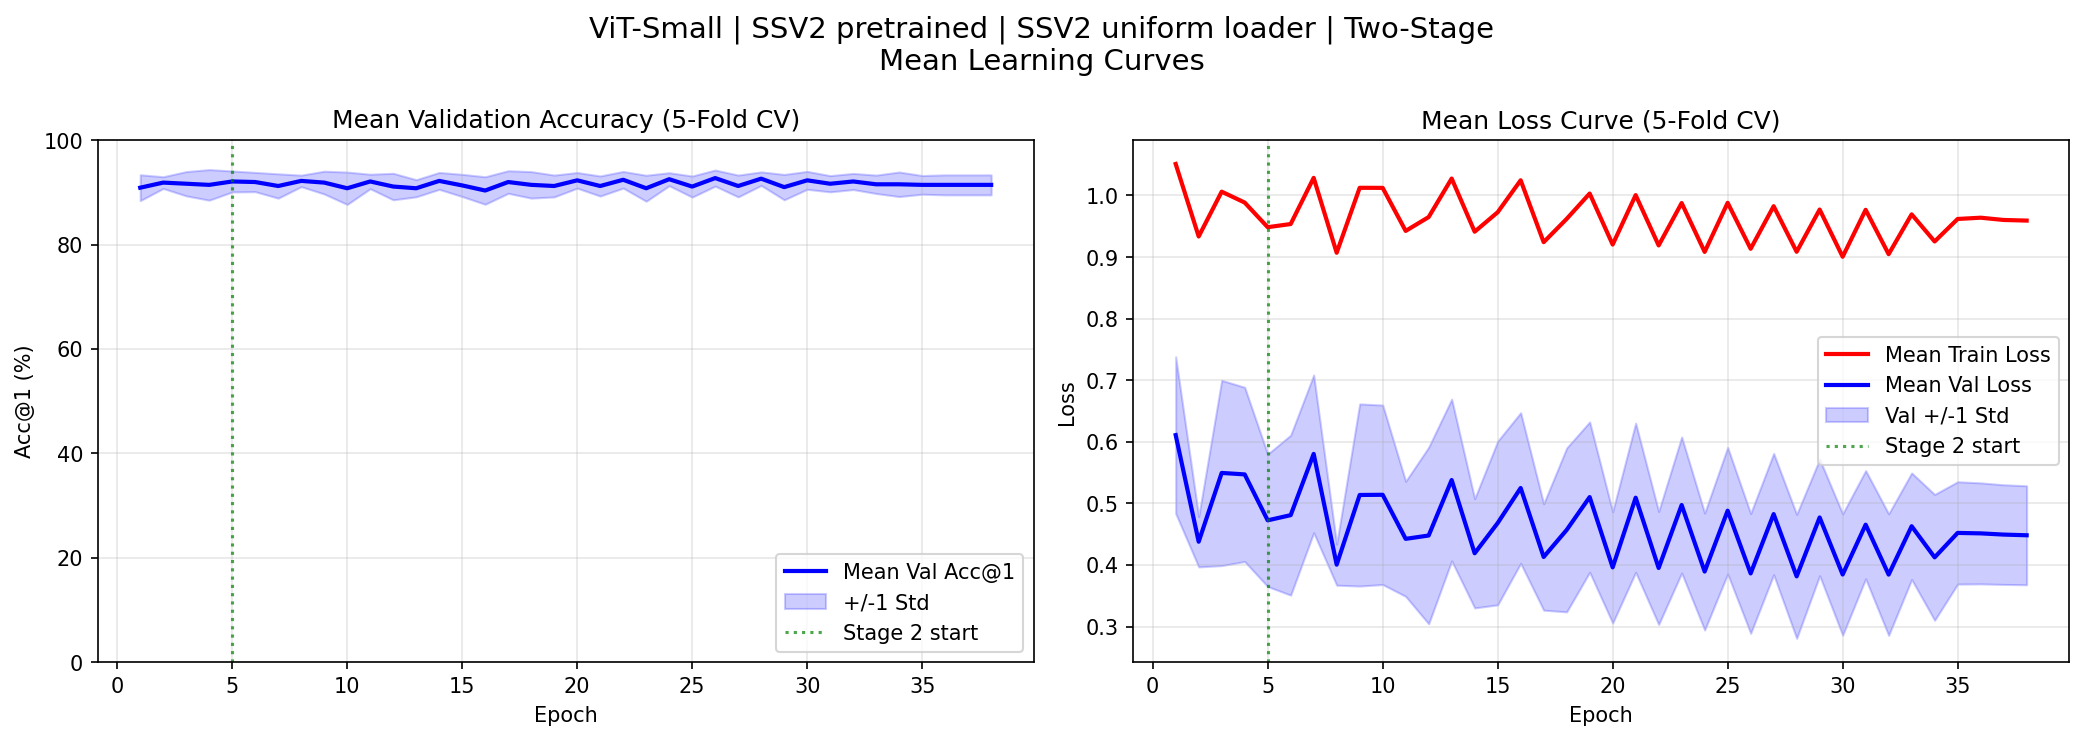
\includegraphics[width=0.95\textwidth]{figure/lc_vits_ssv2_uniform_nomixup.png}
\caption{Kurva pelatihan rata-rata eksperimen E11 (tanpa augmentasi \textit{mixup}/\textit{CutMix}/\textit{reprob})}
\label{fig:4.lc_e11}
\end{figure}

Kurva pelatihan E11 pada Gambar~\ref{fig:4.lc_e11} memperlihatkan konvergensi yang sangat cepat dan stabil, dengan akurasi validasi meningkat tajam sejak epoch-epoch awal dan mencapai kisaran 90\% lebih dalam beberapa puluh epoch pertama. Dibandingkan dengan kurva E5 yang berfluktuasi dan terbatas pada kisaran 60--70\%, kurva E11 jauh lebih konsisten antar fold dengan rentang akurasi validasi yang lebih sempit. Tidak ada tanda-tanda \textit{overfitting} yang berarti, yang mengonfirmasi bahwa tanpa augmentasi pun model tidak terjebak pada data latih secara berlebihan berkat mekanisme regularisasi bawaan AdamW dan strategi \textit{two-stage fine-tune}.\par
Kurva pelatihan E11 pada Gambar~\ref{fig:4.lc_e11} memperlihatkan konvergensi yang sangat cepat dan stabil, dengan akurasi validasi meningkat tajam sejak epoch-epoch awal dan mencapai kisaran 90\% lebih dalam beberapa puluh epoch pertama. Dibandingkan dengan kurva E5 yang berfluktuasi dan terbatas pada kisaran 60--70\%, kurva E11 jauh lebih konsisten antarfold dengan rentang akurasi validasi yang lebih sempit. Tidak ada tanda-tanda \textit{overfitting} yang berarti, yang mengonfirmasi bahwa tanpa augmentasi pun model tidak terjebak pada data latih secara berlebihan berkat mekanisme regularisasi bawaan AdamW dan strategi \textit{two-stage fine-tune}.\par

Gambar~\ref{fig:4.aug_mixup}, Gambar~\ref{fig:4.aug_cutmix}, dan Gambar~\ref{fig:4.aug_reprob} memperlihatkan secara langsung bagaimana masing-masing augmentasi mengubah integritas visual frame gestur SIBI.\par

\begin{figure}[H]
\centering
\begin{subfigure}[t]{0.47\textwidth}
  \centering
  
\includegraphics[width=\linewidth]{figure/aug_mixup_asli.png}
  \caption{Asli: gestur \textit{Aku}}
\end{subfigure}
\hfill
\begin{subfigure}[t]{0.47\textwidth}
  \centering
  
\includegraphics[width=\linewidth]{figure/aug_mixup_hasil.png}
  \caption{\textit{Mixup} ($\lambda{=}0.5$): perpaduan piksel \textit{Aku} + \textit{Bapak}}
\end{subfigure}

\caption{Ilustrasi efek augmentasi \textit{Mixup} pada frame gestur SIBI}
\label{fig:4.aug_mixup}
\end{figure}

\begin{figure}[H]
\centering
\begin{subfigure}[t]{0.47\textwidth}
  \centering
  
\includegraphics[width=\linewidth]{figure/aug_cutmix_asli.png}
  \caption{Asli: gestur \textit{Aku}}
\end{subfigure}
\hfill
\begin{subfigure}[t]{0.47\textwidth}
  \centering
  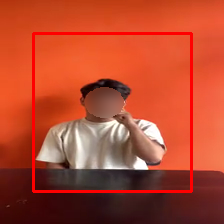
\includegraphics[width=\linewidth]{figure/aug_cutmix_hasil.png}
  \caption{\textit{CutMix} ($\lambda{=}0.5$): region dari \textit{Bapak} ditempel ke \textit{Aku}}
\end{subfigure}

\caption{Ilustrasi efek augmentasi \textit{CutMix} pada frame gestur SIBI}
\label{fig:4.aug_cutmix}
\end{figure}

\begin{figure}[H]
\centering
\begin{subfigure}[t]{0.47\textwidth}
  \centering
  
\includegraphics[width=\linewidth]{figure/aug_erase_asli.png}
  \caption{Asli: gestur \textit{Aku}}
\end{subfigure}
\hfill
\begin{subfigure}[t]{0.47\textwidth}
  \centering
  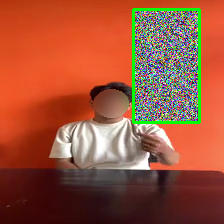
\includegraphics[width=\linewidth]{figure/aug_erase_hasil.png}
  \caption{\textit{Random Erasing}: area tangan digantikan \textit{noise} piksel acak}
\end{subfigure}

\caption{Ilustrasi efek augmentasi \textit{Random Erasing} pada frame gestur SIBI}
\label{fig:4.aug_reprob}
\end{figure}

Hasil ini mengungkap alasan mendasar mengapa augmentasi berdampak negatif pada pengenalan gestur SIBI: ketiga teknik tersebut secara langsung merusak konteks gerakan detail yang menjadi ciri pembeda antar isyarat. \textit{Mixup} dan \textit{CutMix} mencampur dua klip video beserta labelnya secara proporsional, sehingga gerakan tangan yang memiliki trajektori dan posisi jari yang spesifik, seperti perbedaan halus antara gestur \textit{Kamu}, \textit{Aku}, dan \textit{Bapak} yang seluruhnya melibatkan gerakan tangan menuju referensi tertentu, menjadi tercampur dan tidak lagi merepresentasikan pola spasio-temporal yang koheren. Model dipaksa mempelajari transisi antara dua gestur yang berbeda alih-alih mengenali karakteristik unik masing-masing gestur. \textit{Reprob} (\textit{random erasing}) memperburuk masalah ini dengan menghapus area frame secara acak, yang pada video gestur tangan berpotensi menghilangkan informasi kritis seperti posisi jari, orientasi telapak tangan, atau kecepatan pergerakan pada momen tertentu, detail yang justru merupakan pembeda utama antar kelas SIBI. Karena gestur bahasa isyarat sangat bergantung pada sekuens spasio-temporal yang utuh dan terstruktur, setiap gangguan pada kontinuitas gerakan tersebut menghilangkan konteks yang dibutuhkan model untuk membangun representasi diskriminatif yang akurat. Dengan menonaktifkan ketiga augmentasi ini, model dapat mempelajari seluruh pola gerakan secara penuh dari sampel asli, sehingga mampu menangkap detail halus yang membedakan satu gestur dari yang lain.\par

Berdasarkan hasil ini, E11 ditetapkan sebagai konfigurasi VideoMAE terbaik dalam penelitian ini dan menjadi acuan pada perbandingan lintas arsitektur di bagian berikutnya.\par

%===========================================================================
\subsection{Perbandingan Lintas Arsitektur: VideoMAE, ViViT, dan I3D} \label{IV.Sek6}
%===========================================================================

Bagian ini membandingkan empat konfigurasi model secara lintas arsitektur untuk mengevaluasi posisi relatif VideoMAE terhadap model video lainnya pada dataset SIBI. Empat model yang dibandingkan adalah: (1) E11, VideoMAE ViT-Small dengan bobot SSV2 dan \textit{uniform sampling}, (2) E12, VideoMAE ViT-Base dengan bobot K400 dan \textit{Kinetics loader} (\textit{dense sampling}), (3) ViViT-B/16x2 yang di-\textit{fine-tune} dari bobot K400, serta (4) I3D (\textit{Inflated 3D ConvNet}) yang dilatih menggunakan bobot \textit{pre-train} ImageNet. ViViT (\textit{Video Vision Transformer}) merupakan model \textit{Transformer} berbasis \textit{tubelet embedding} yang mengolah video sebagai urutan \textit{patch} spasio-temporal secara langsung tanpa \textit{masked autoencoding pre-training}, sedangkan I3D merupakan model berbasis arsitektur 3D CNN yang secara historis terbukti efektif pada dataset aksi video berskala kecil berkat \textit{local inductive bias} yang kuat. Konfigurasi lengkap disajikan pada Tabel~\ref{tab:4.s6_config}.\par
Empat model yang dibandingkan adalah (1) E11, VideoMAE ViT-Small dengan bobot SSV2 dan \textit{uniform sampling}, (2) E12, VideoMAE ViT-Base dengan bobot K400 dan \textit{Kinetics loader} (\textit{dense sampling}), (3) ViViT-B/16x2 yang di-\textit{fine-tune} dari bobot K400, serta (4) I3D (\textit{Inflated 3D ConvNet}) yang dilatih menggunakan bobot \textit{pre-train} ImageNet. ViViT (\textit{Video Vision Transformer}) merupakan model \textit{Transformer} berbasis \textit{tubelet embedding} yang mengolah video sebagai urutan \textit{patch} spasio-temporal secara langsung tanpa \textit{masked autoencoding pre-training}, sedangkan I3D merupakan model berbasis arsitektur 3D CNN yang secara historis terbukti efektif pada dataset aksi video berskala kecil berkat \textit{local inductive bias} yang kuat. Konfigurasi lengkap disajikan pada Tabel~\ref{tab:4.s6_config}.\par

\begin{table}[H]
\centering
\caption{Konfigurasi eksperimen perbandingan lintas arsitektur: E11, E12, ViViT, dan I3D}
\label{tab:4.s6_config}
{\setlength{\tabcolsep}{3pt}
\footnotesize
\begin{tabular}{|l|l|l|l|l|}
\hline
\rowcolor{gray!15} \multicolumn{1}{|c|}{\textbf{Parameter}} & \multicolumn{1}{c|}{\textbf{E11}} & \multicolumn{1}{c|}{\textbf{E12}} & \multicolumn{1}{c|}{\textbf{ViViT}} & \multicolumn{1}{c|}{\textbf{I3D}} \\
\hline
\makecell[l]{Arsitektur\\Model} & \makecell[l]{VideoMAE\\ViT-Small} & \makecell[l]{VideoMAE\\ViT-Base} & \multicolumn{1}{l|}{ViViT-B/16x2} & \makecell[l]{I3D (Inflated\\3D ConvNet)} \\
\hline
\makecell[l]{Dataset\\\textit{Pre-train}} & \multicolumn{1}{l|}{SSV2} & \multicolumn{1}{l|}{Kinetics-400} & \multicolumn{1}{l|}{Kinetics-400} & \multicolumn{1}{l|}{ImageNet} \\
\hline
\makecell[l]{Strategi\\\textit{Sampling}} & \makecell[l]{\textit{Uniform}\\(SSV2 loader)} & \makecell[l]{\textit{Dense}\\(Kin. loader)} & \multicolumn{1}{l|}{Seragam} & \makecell[l]{Seluruh video\\(RGB)} \\
\hline
\makecell[l]{\textit{Epoch}\\Total} & \multicolumn{1}{r|}{55 (5 + 50)} & \multicolumn{1}{r|}{55 (5 + 50)} & \multicolumn{1}{r|}{55} & \multicolumn{1}{r|}{55} \\
\hline
\makecell[l]{Jumlah\\\textit{Frame}} & \multicolumn{1}{r|}{16} & \multicolumn{1}{r|}{16} & \multicolumn{1}{r|}{32} & \multicolumn{1}{r|}{64} \\
\hline
\makecell[l]{\textit{Learning}\\Rate} & \multicolumn{1}{r|}{$10^{-3}$} & \multicolumn{1}{r|}{$10^{-3}$} & \multicolumn{1}{r|}{$10^{-3}$} & \multicolumn{1}{r|}{$10^{-3}$} \\
\hline
\makecell[l]{\textit{Hyperparameter}\\Lain} & \multicolumn{4}{c|}{Sama dengan Tabel~\ref{tab:4.umum_config}} \\
\hline
\end{tabular}
}
\end{table}

\begin{table}[H]
\centering
\caption{Nilai \textit{Best Val Acc@1} (\%) per fold dan ringkasan hasil perbandingan lintas arsitektur}
\label{tab:4.s6_fold}
{\setlength{\tabcolsep}{3pt}
\footnotesize
\begin{tabular}{|l|r|r|r|r|r|r|r|}
\hline
\rowcolor{gray!15} \multicolumn{1}{|c|}{Kode} & \multicolumn{1}{c|}{Fold 1} & \multicolumn{1}{c|}{Fold 2} & \multicolumn{1}{c|}{Fold 3} & \multicolumn{1}{c|}{Fold 4} & \multicolumn{1}{c|}{Fold 5} & \multicolumn{1}{c|}{\makecell[c]{Rata-\\rata}} & \multicolumn{1}{c|}{Terbaik} \\
\hline
\rowcolor{highlightpink}E11   & 94.05 & 94.57 & 92.43 & 95.68 & 92.97 & 93.94 & 95.68 \\
\hline
\rowcolor{highlightgreen}E12   & 97.84 & 95.11 & 97.84 & 98.92 & 96.22 & 97.18 & 98.92 \\
\hline
ViViT & 95.14 & 96.20 & 95.68 & 95.14 & 91.89 & 94.81 & 96.20 \\
\hline
I3D   & 98.38 & 96.74 & 96.22 & 97.30 & 95.68 & 96.86 & 98.38 \\
\hline
\end{tabular}
}
\end{table}

Tabel~\ref{tab:4.s6_fold} menunjukkan bahwa E12 (VideoMAE ViT-Base + K400) mencapai performa terbaik dengan rata-rata akurasi 97.18\%, diikuti I3D (96.86\%), ViViT (94.81\%), dan E11 (93.94\%). Selisih antar keempat model berkisar 0.32--3.24 poin persentase, mengindikasikan bahwa seluruh model berada dalam rentang performa yang kompetitif. Keunggulan E12 atas I3D yang hanya 0.32 poin persentase sangat signifikan: VideoMAE berbasis \textit{Transformer} dengan konfigurasi yang tepat mampu menyamai bahkan sedikit melampaui arsitektur 3D CNN yang secara historis unggul pada dataset kecil. Variabilitas antar fold pada E12 (95.11\%--98.92\%) sedikit lebih besar dibandingkan I3D (95.68\%--98.38\%), namun rata-rata E12 tetap unggul di semua fold kecuali Fold 2 di mana ViViT (96.20\%) mengungguli E12 (95.11\%). I3D menunjukkan konsistensi yang sangat tinggi antar fold (95.68\%--98.38\%), yang mencerminkan kemantapan \textit{local inductive bias} arsitektur CNN pada dataset berskala kecil.\par
Tabel~\ref{tab:4.s6_fold} menunjukkan bahwa E12 (VideoMAE ViT-Base + K400) mencapai performa terbaik dengan rata-rata akurasi 97.18\%, diikuti I3D (96.86\%), ViViT (94.81\%), dan E11 (93.94\%). Selisih antar keempat model berkisar 0.32--3.24 poin persentase, mengindikasikan bahwa seluruh model berada dalam rentang performa yang kompetitif. Keunggulan E12 atas I3D yang hanya 0.32 poin persentase sangat signifikan: VideoMAE berbasis \textit{Transformer} dengan konfigurasi yang tepat mampu menyamai bahkan sedikit melampaui arsitektur 3D CNN yang secara historis unggul pada dataset kecil. Variabilitas antarfold pada E12 (95.11\%--98.92\%) sedikit lebih besar dibandingkan I3D (95.68\%--98.38\%), namun rata-rata E12 tetap unggul di semua fold kecuali Fold 2 di mana ViViT (96.20\%) mengungguli E12 (95.11\%). I3D menunjukkan konsistensi yang sangat tinggi antarfold (95.68\%--98.38\%), yang mencerminkan kemantapan \textit{local inductive bias} arsitektur CNN pada dataset berskala kecil.\par

Gambar~\ref{fig:4.lc_e12}, Gambar~\ref{fig:4.lc_vivit}, dan Gambar~\ref{fig:4.lc_i3d} menampilkan kurva pelatihan rata-rata untuk E12, ViViT, dan I3D.\par

\begin{figure}[H]
\centering
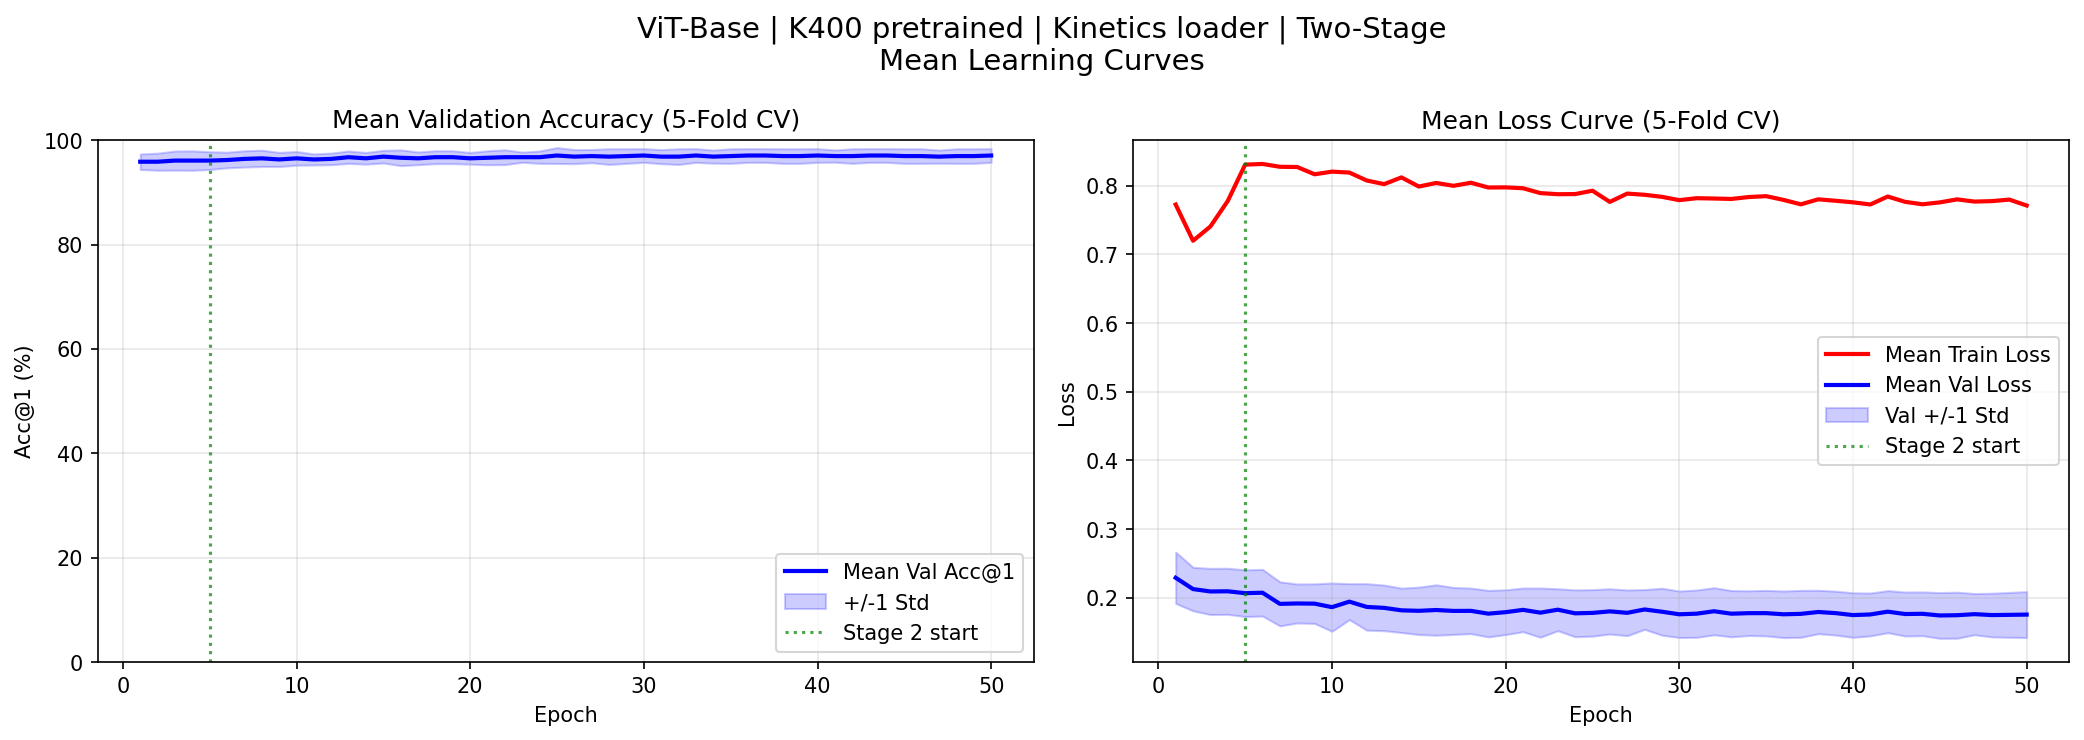
\includegraphics[width=0.95\textwidth]{figure/lc_vitb_k400_dense_nomixup.png}
\caption{Kurva pelatihan rata-rata eksperimen E12 (VideoMAE ViT-Base + K400)}
\label{fig:4.lc_e12}
\end{figure}

Kurva pelatihan E12 pada Gambar~\ref{fig:4.lc_e12} memperlihatkan konvergensi yang cepat dan stabil sejak epoch-epoch awal \textit{stage} 2, konsisten dengan hasil E11. Akurasi validasi mencapai kisaran 95\% lebih dalam beberapa puluh epoch pertama dan terus meningkat secara bertahap hingga akhir pelatihan. Variasi antar fold relatif kecil, mencerminkan bahwa bobot K400 pada ViT-Base memberikan representasi awal yang kuat dan konsisten untuk domain gestur tangan. Tidak ditemukan tanda-tanda \textit{overfitting} pada kurva ini, mengonfirmasi bahwa mekanisme regularisasi yang diterapkan cukup efektif meskipun augmentasi dinonaktifkan.\par
Kurva pelatihan E12 pada Gambar~\ref{fig:4.lc_e12} memperlihatkan konvergensi yang cepat dan stabil sejak epoch-epoch awal \textit{stage} 2, konsisten dengan hasil E11. Akurasi validasi mencapai kisaran 95\% lebih dalam beberapa puluh epoch pertama dan terus meningkat secara bertahap hingga akhir pelatihan. Variasi antarfold relatif kecil, mencerminkan bahwa bobot K400 pada ViT-Base memberikan representasi awal yang kuat dan konsisten untuk domain gestur tangan. Tidak ditemukan tanda-tanda \textit{overfitting} pada kurva ini, mengonfirmasi bahwa mekanisme regularisasi yang diterapkan cukup efektif meskipun augmentasi dinonaktifkan.\par

\begin{figure}[H]
\centering
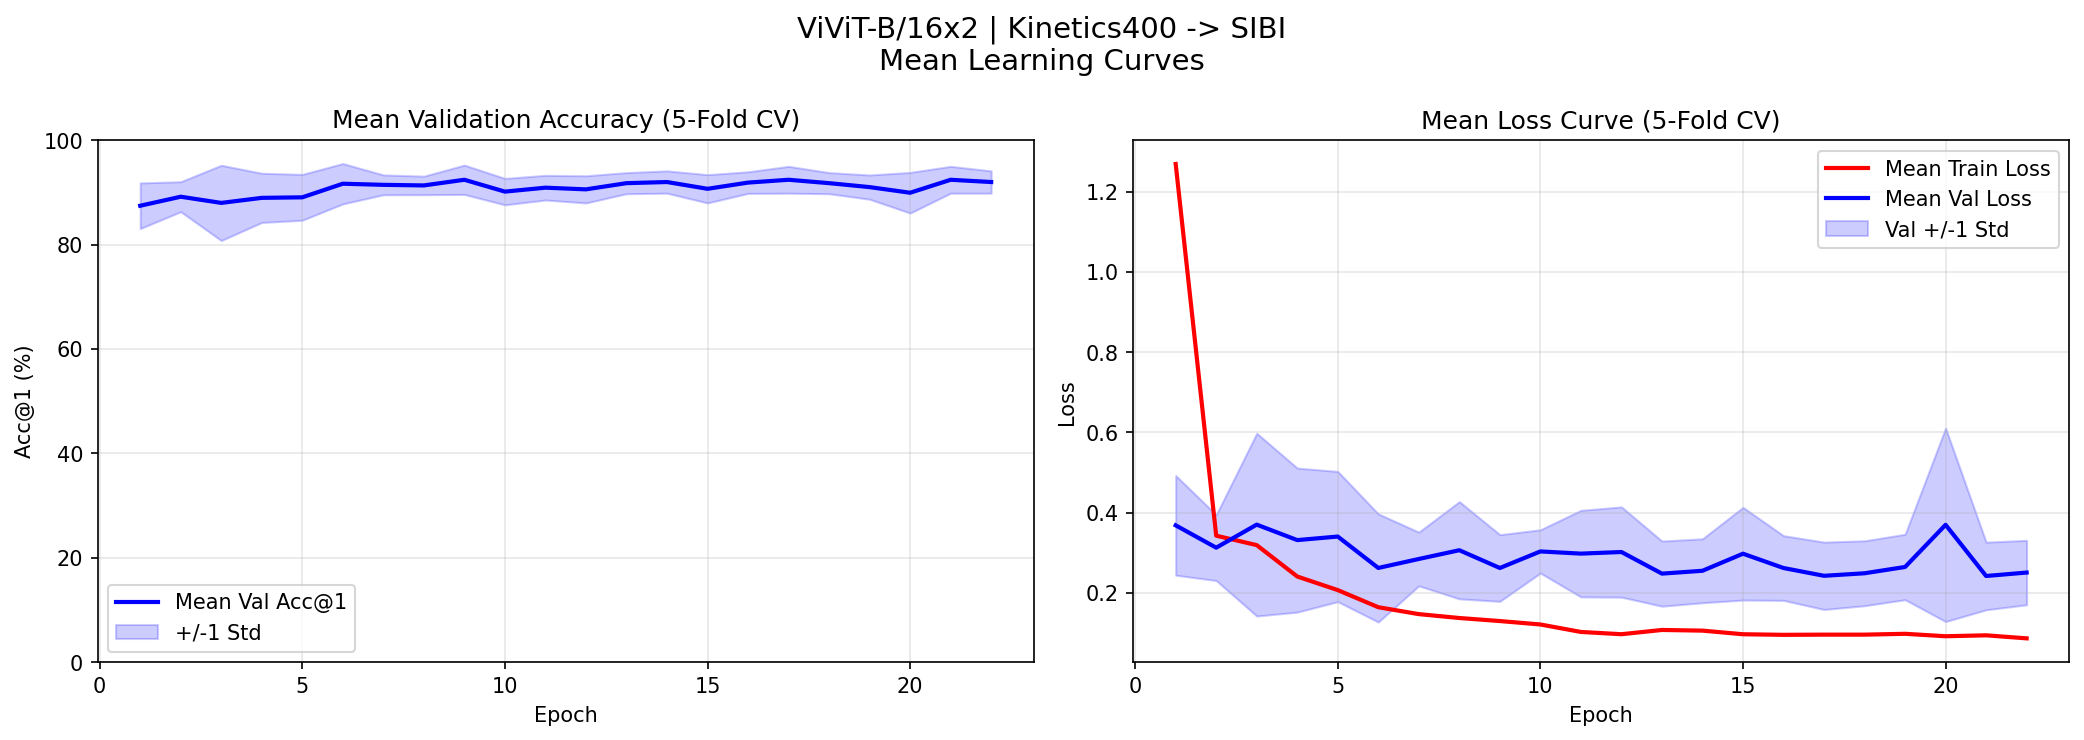
\includegraphics[width=0.95\textwidth]{figure/lc_vivit.png}
\caption{Kurva pelatihan rata-rata model ViViT-B/16x2 (5-Fold)}
\label{fig:4.lc_vivit}
\end{figure}

Kurva pelatihan ViViT pada Gambar~\ref{fig:4.lc_vivit} menunjukkan pola yang berbeda dari E11 dan E12: konvergensi terjadi lebih cepat namun disertai fluktuasi yang lebih besar antar fold, terutama pada Fold 5 yang menghasilkan akurasi validasi lebih rendah (91.89\%). Penggunaan \textit{early stopping} dengan kesabaran 5 epoch membuat beberapa fold berhenti relatif lebih awal, yang berkontribusi pada variabilitas antar fold yang lebih tinggi. Meski demikian, kurva ViViT secara keseluruhan menunjukkan kemampuan konvergensi yang baik dalam 55 epoch, mengonfirmasi bahwa bobot K400 juga efektif sebagai titik awal \textit{fine-tune} untuk ViViT pada dataset SIBI.\par
Kurva pelatihan ViViT pada Gambar~\ref{fig:4.lc_vivit} menunjukkan pola yang berbeda dari E11 dan E12: konvergensi terjadi lebih cepat namun disertai fluktuasi yang lebih besar antarfold, terutama pada Fold 5 yang menghasilkan akurasi validasi lebih rendah (91.89\%). Penggunaan \textit{early stopping} dengan kesabaran 5 epoch membuat beberapa fold berhenti relatif lebih awal, yang berkontribusi pada variabilitas antarfold yang lebih tinggi. Meski demikian, kurva ViViT secara keseluruhan menunjukkan kemampuan konvergensi yang baik dalam 55 epoch, mengonfirmasi bahwa bobot K400 juga efektif sebagai titik awal \textit{fine-tune} untuk ViViT pada dataset SIBI.\par

\begin{figure}[H]
\centering
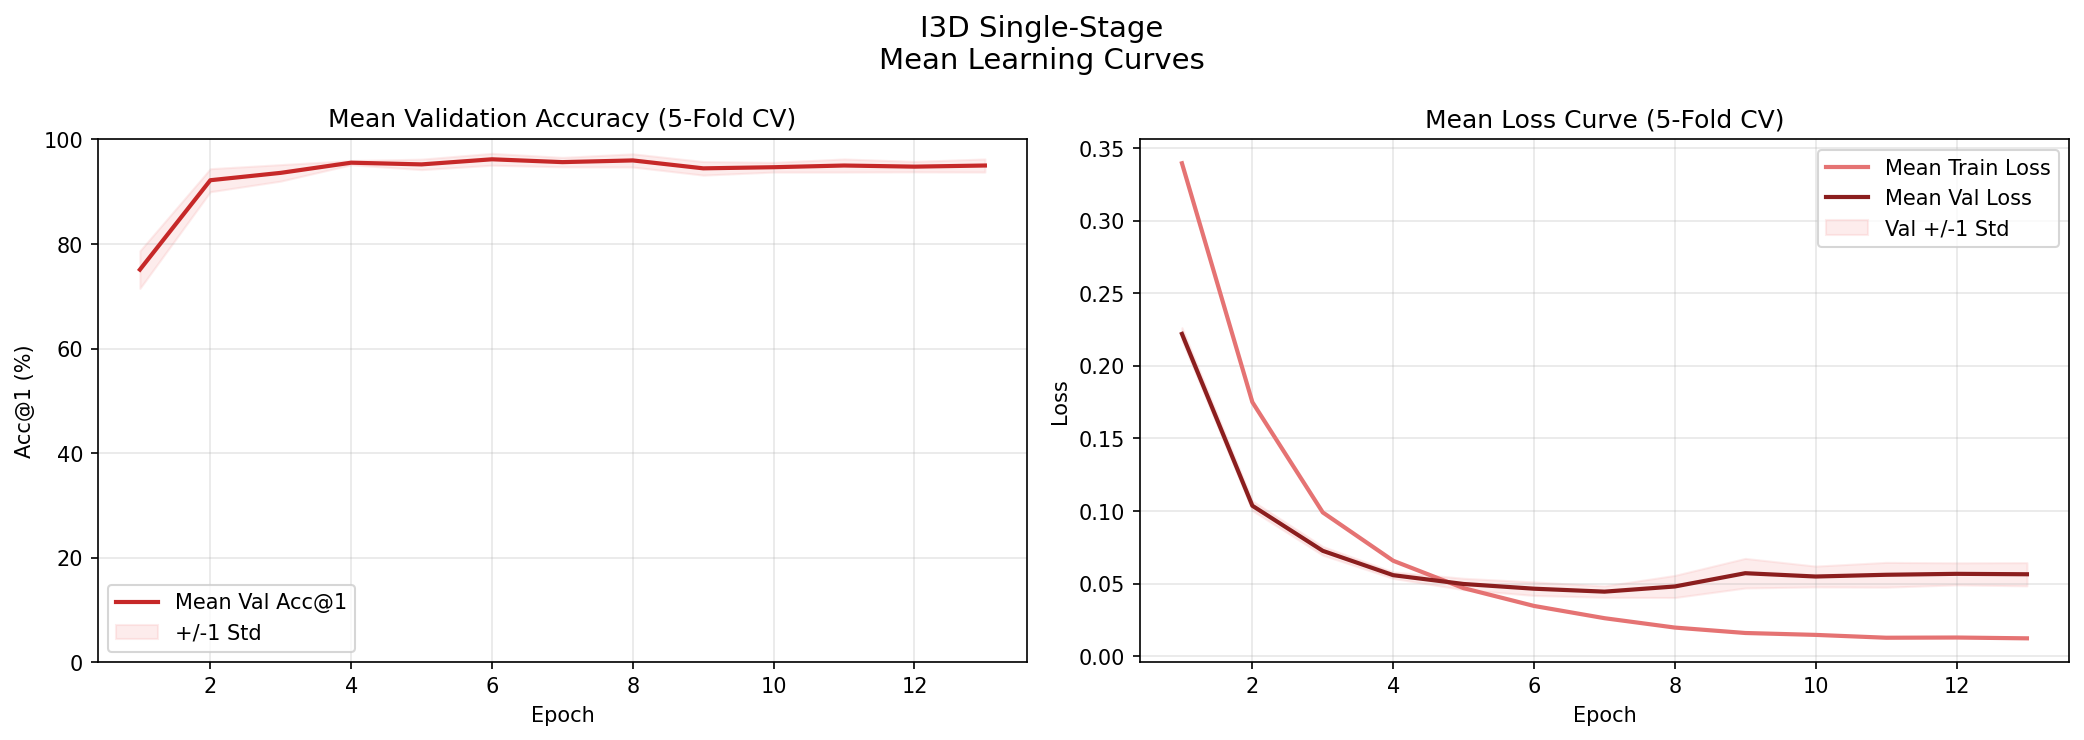
\includegraphics[width=0.95\textwidth]{figure/lc_i3d.png}
\caption{Kurva pelatihan rata-rata model I3D \textit{baseline} (5-Fold)}
\label{fig:4.lc_i3d}
\end{figure}

Kurva pelatihan I3D pada Gambar~\ref{fig:4.lc_i3d} memperlihatkan konvergensi yang sangat cepat dan stabil: akurasi validasi melonjak tajam sejak epoch-epoch pertama dan mencapai nilai di atas 90\% hanya dalam beberapa epoch pelatihan. Pola ini mencerminkan karakteristik model berbasis 3D CNN yang diinisialisasi dengan bobot ImageNet, representasi awal dari domain gambar alami sudah cukup kuat untuk langsung disesuaikan (\textit{fine-tune}) pada domain gestur tangan dengan data yang terbatas. Tidak ada tanda-tanda \textit{overfitting} yang signifikan, karena \textit{training loss} dan \textit{validation accuracy} bergerak secara sinkron menuju konvergensi sebelum akhirnya dihentikan oleh mekanisme \textit{early stopping} dalam 9--13 epoch per fold. Kecepatan konvergensi I3D yang jauh lebih tinggi dibandingkan model-model berbasis \textit{Transformer} (E11, E12, ViViT) menunjukkan keunggulan \textit{inductive bias} lokal CNN dalam memanfaatkan representasi tekstur dan bentuk dari bobot ImageNet secara efisien pada dataset berskala kecil.\par

Tabel~\ref{tab:4.s6_perkelas_vivit} dan Tabel~\ref{tab:4.s6_perkelas_i3d} menyajikan laporan klasifikasi per kelas gabungan seluruh fold untuk model ViViT dan I3D.\par

\begin{table}[H]
\centering
\caption{Laporan klasifikasi per kelas (gabungan semua fold) model ViViT-B/16x2}
\label{tab:4.s6_perkelas_vivit}
\footnotesize
\begin{tabular}{|l|r|r|r|r|}
\hline
\rowcolor{gray!15} \multicolumn{1}{|c|}{Kelas} & \multicolumn{1}{c|}{Presisi} & \multicolumn{1}{c|}{\textit{Recall}} & \multicolumn{1}{c|}{F1-\textit{Score}} & \multicolumn{1}{c|}{\textit{Support}} \\
\hline
Aku     & 0.94 & 0.97 & 0.95 & 90 \\
Bapak   & 0.94 & 0.93 & 0.94 & 90 \\
Bawa    & 0.99 & 0.99 & 0.99 & 88 \\
Guru    & 0.99 & 1.00 & 0.99 & 90 \\
Ibu     & 0.92 & 0.97 & 0.94 & 96 \\
Kamu    & 0.96 & 0.94 & 0.95 & 93 \\
Mau     & 0.88 & 0.91 & 0.90 & 99 \\
Pulang  & 0.98 & 0.95 & 0.96 & 99 \\
Sekolah & 0.99 & 0.98 & 0.98 & 89 \\
Suka    & 0.91 & 0.86 & 0.88 & 90 \\
\hline
\textit{Macro} Avg & 0.95 & 0.95 & 0.95 & 924 \\
\hline
\end{tabular}
\end{table}

\begin{table}[H]
\centering
\caption{Laporan klasifikasi per kelas (gabungan semua fold) model I3D \textit{baseline}}
\label{tab:4.s6_perkelas_i3d}
\footnotesize
\begin{tabular}{|l|r|r|r|r|}
\hline
\rowcolor{gray!15} \multicolumn{1}{|c|}{Kelas} & \multicolumn{1}{c|}{Presisi} & \multicolumn{1}{c|}{\textit{Recall}} & \multicolumn{1}{c|}{F1-\textit{Score}} & \multicolumn{1}{c|}{\textit{Support}} \\
\hline
Aku     & 0.94 & 0.99 & 0.96 & 90 \\
Bapak   & 1.00 & 0.98 & 0.99 & 90 \\
Bawa    & 1.00 & 1.00 & 1.00 & 88 \\
Guru    & 0.99 & 1.00 & 0.99 & 90 \\
Ibu     & 0.98 & 1.00 & 0.99 & 96 \\
Kamu    & 0.98 & 0.98 & 0.98 & 93 \\
Mau     & 0.89 & 0.91 & 0.90 & 99 \\
Pulang  & 0.99 & 0.97 & 0.98 & 99 \\
Sekolah & 0.99 & 0.99 & 0.99 & 89 \\
Suka    & 0.94 & 0.88 & 0.91 & 90 \\
\hline
\textit{Macro} Avg & 0.97 & 0.97 & 0.97 & 924 \\
\hline
\end{tabular}
\end{table}

Tabel~\ref{tab:4.s6_perkelas_vivit} menunjukkan kinerja ViViT yang merata di seluruh kelas dengan F1-\textit{score} minimum 0.88 (kelas \textit{Suka}) dan maksimum 0.99 (kelas \textit{Bawa} dan \textit{Guru}). Tabel~\ref{tab:4.s6_perkelas_i3d} memperlihatkan keunggulan I3D yang lebih tinggi lagi dengan F1-\textit{score} minimum 0.90 (kelas \textit{Mau}), bahkan kelas-kelas yang paling sulit bagi VideoMAE E5 seperti \textit{Suka} (F1=0.91), \textit{Pulang} (F1=0.98), dan \textit{Sekolah} (F1=0.99) dapat diklasifikasikan I3D dengan F1 di atas 0.90. Kelas \textit{Bawa} mencapai F1=1.00 pada I3D, mengonfirmasi bahwa gestur ini memiliki karakteristik visual yang sangat kuat. \textit{Macro} F1 I3D (0.97) lebih tinggi dari ViViT (0.95), namun keduanya jauh melampaui VideoMAE E5 (0.60), mengindikasikan bahwa penonaktifan augmentasi (sebagaimana pada E11 dan E12) merupakan faktor paling krusial dalam meningkatkan performa model pada dataset SIBI.\par

Gambar~\ref{fig:4.cm_e12}, Gambar~\ref{fig:4.cm_vivit}, dan Gambar~\ref{fig:4.cm_i3d} menampilkan \textit{confusion matrix} gabungan seluruh fold untuk E12, ViViT, dan I3D.\par

\begin{figure}[H]
\centering
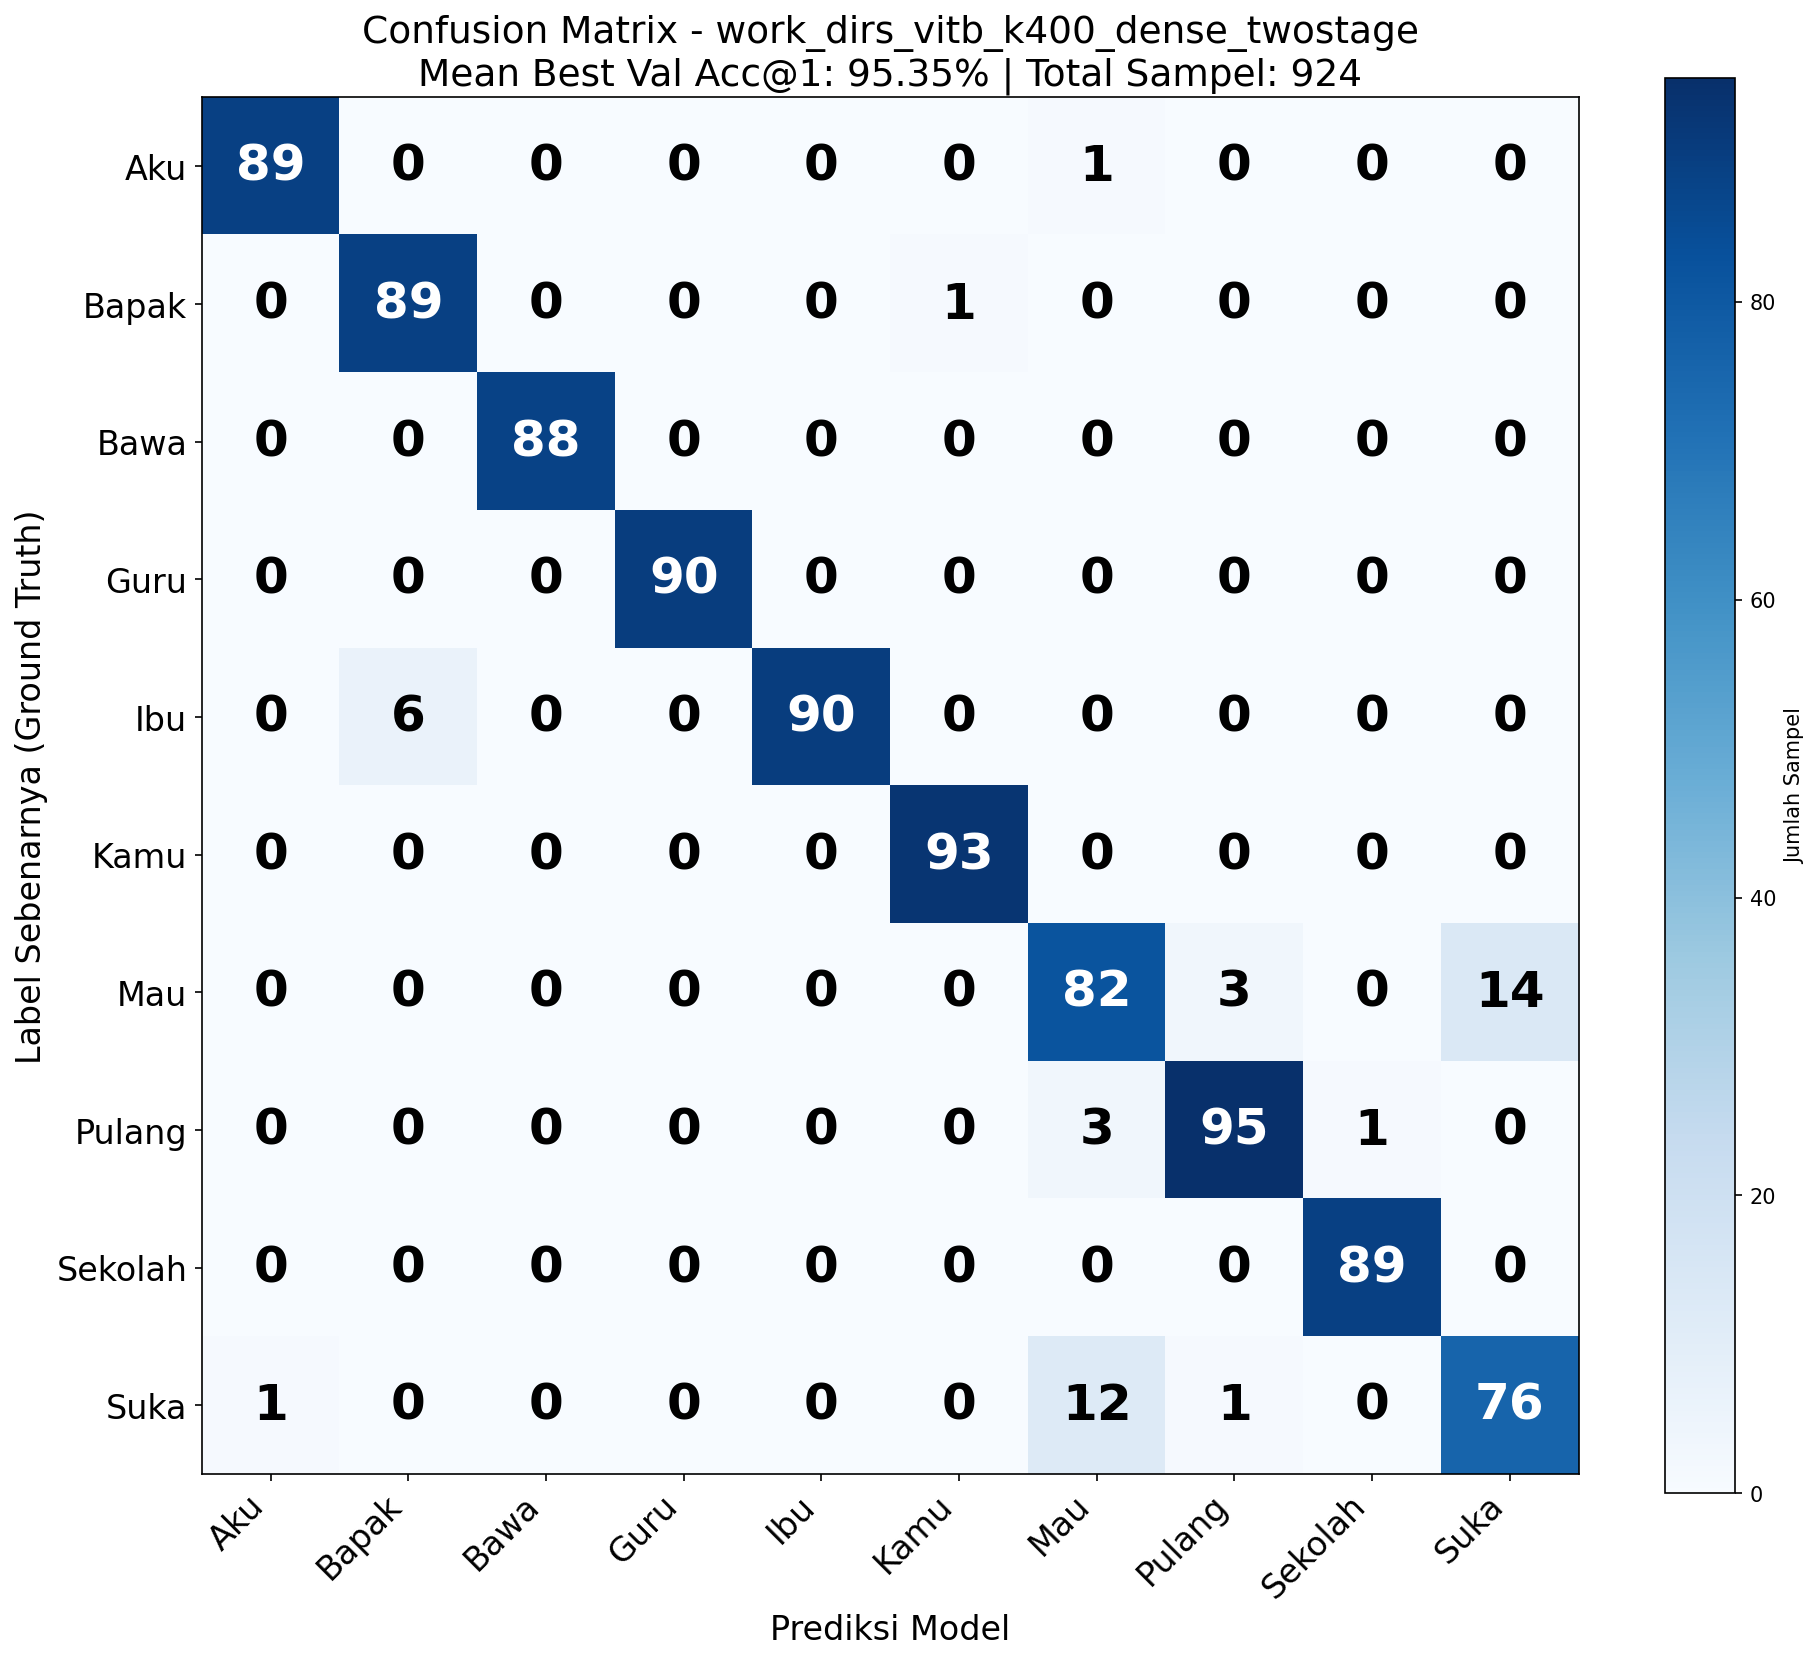
\includegraphics[width=0.95\textwidth]{figure/cm_vitb_k400_dense_nomixup_new_font.png}
\caption{\textit{Confusion matrix} gabungan semua fold eksperimen E12 (VideoMAE ViT-Base + K400)}
\label{fig:4.cm_e12}
\end{figure}

\textit{Confusion matrix} E12 pada Gambar~\ref{fig:4.cm_e12} menampilkan diagonal yang sangat dominan dengan intensitas tinggi hampir seragam di seluruh kelas. Sel-sel di luar diagonal sangat jarang bernilai tinggi, mencerminkan akurasi 97.18\% yang tinggi secara merata. Beberapa kesalahan kecil masih tampak pada kelas \textit{Mau} dan kelas yang berdekatan secara semantik, namun intensitasnya sangat rendah dibandingkan nilai diagonal. Dibandingkan dengan \textit{confusion matrix} E5 (Gambar~\ref{fig:4.cm_e5}), perubahan ini sangat dramatis, memperlihatkan bahwa kombinasi ViT-Base, bobot K400, dan penonaktifan augmentasi menghasilkan kemampuan diskriminasi yang hampir setara dengan I3D.\par

\begin{figure}[H]
\centering
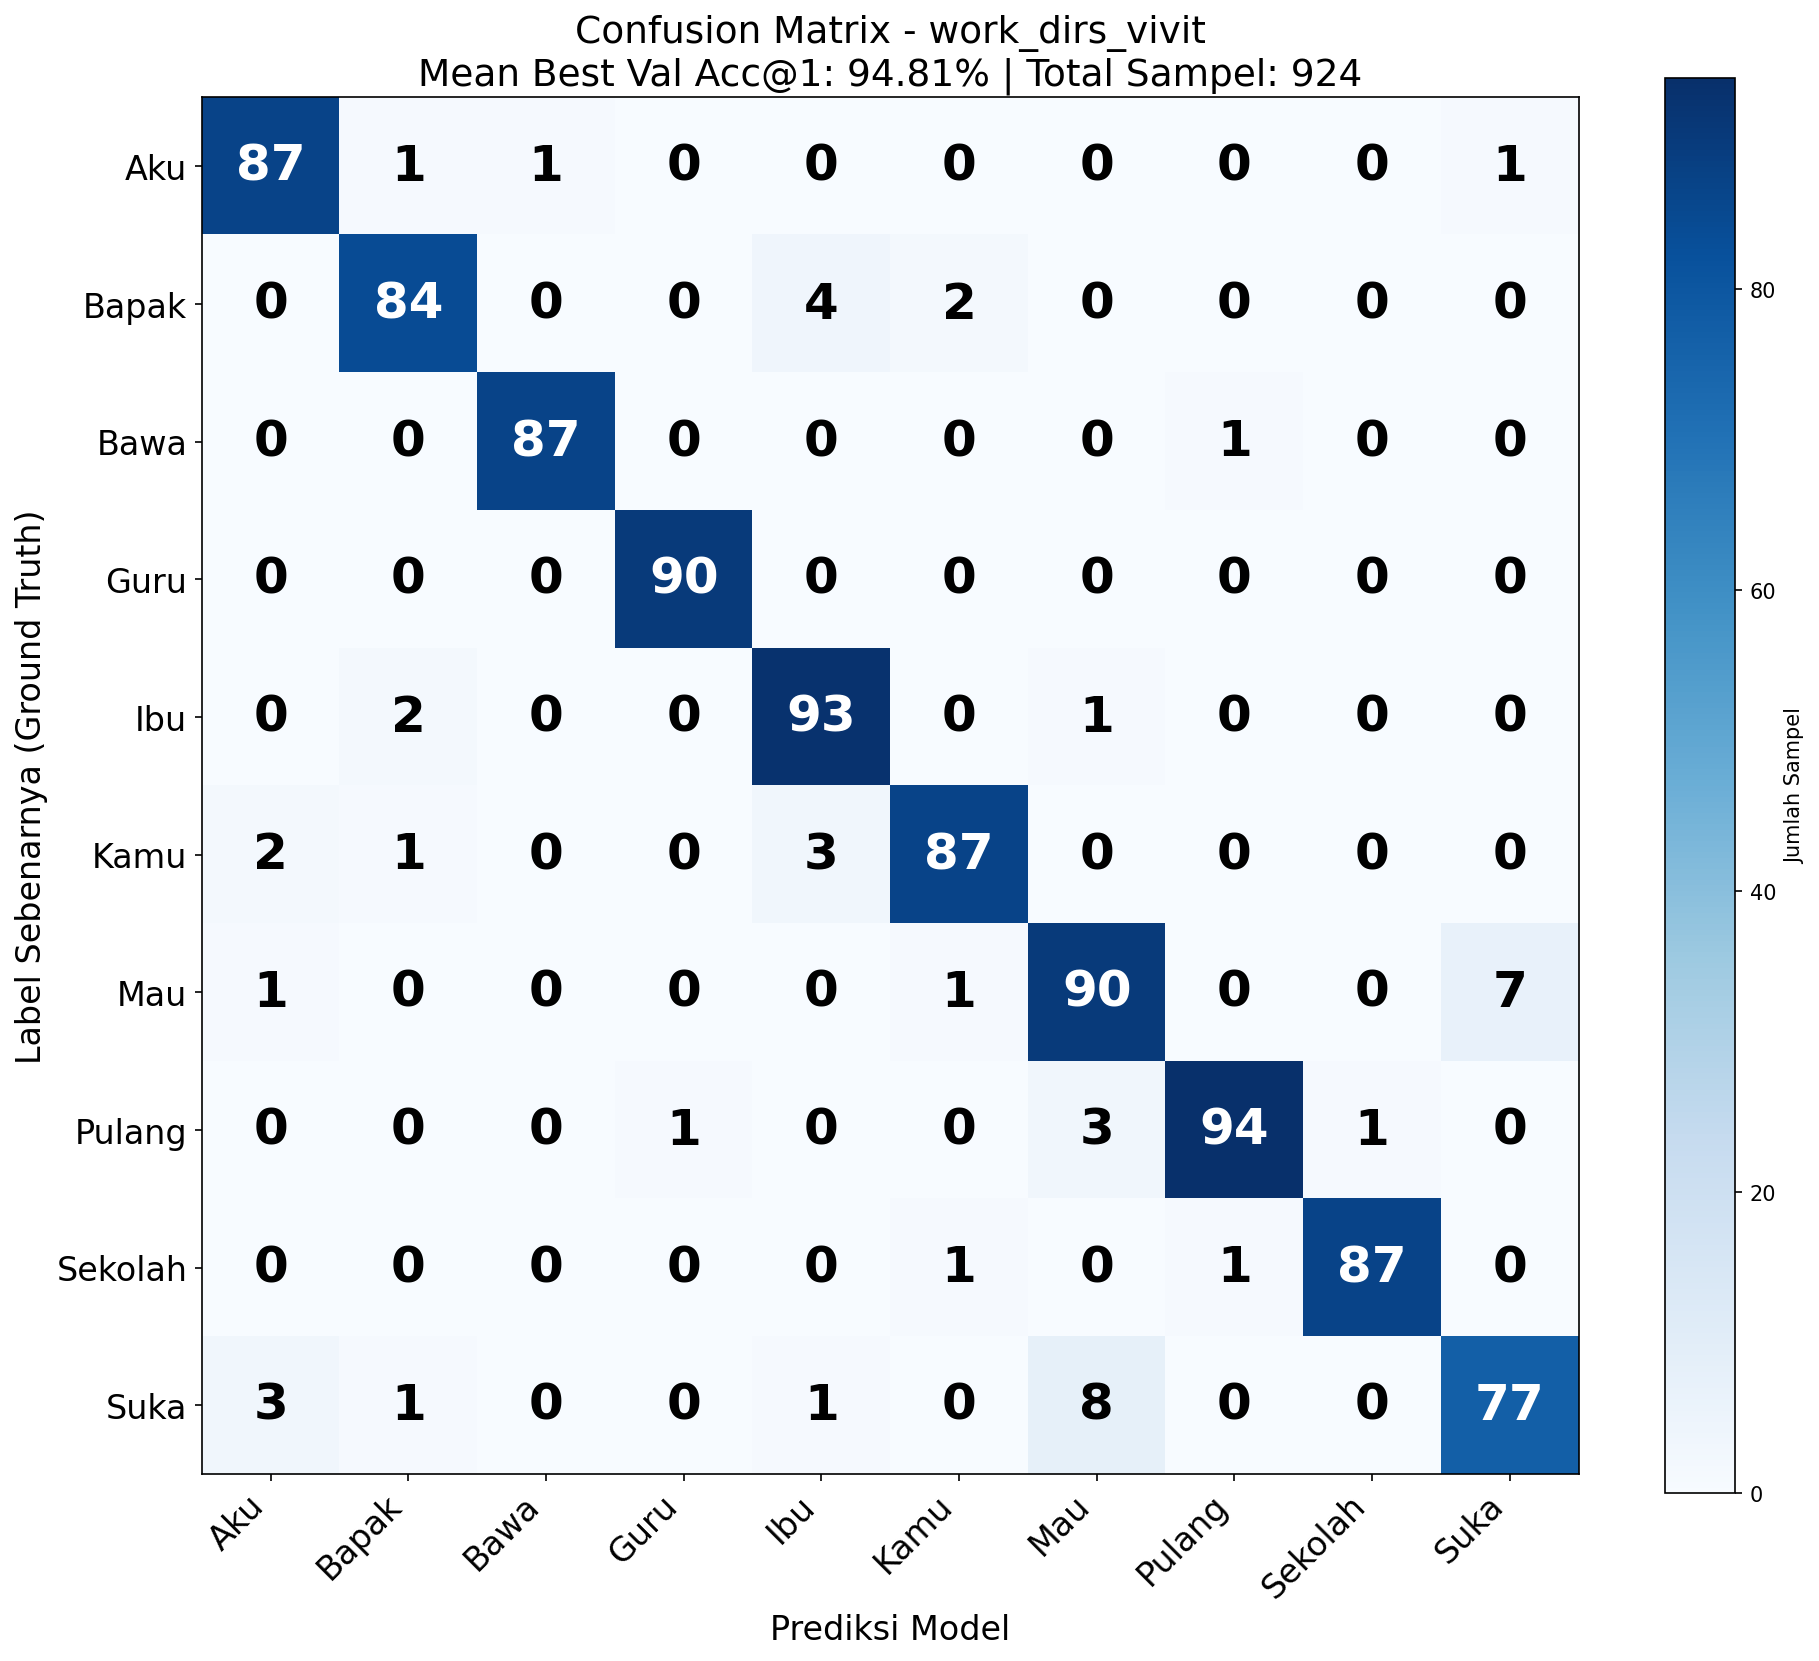
\includegraphics[width=0.95\textwidth]{figure/cm_vivit_new_font.png}
\caption{\textit{Confusion matrix} gabungan semua fold model ViViT-B/16x2}
\label{fig:4.cm_vivit}
\end{figure}

\textit{Confusion matrix} ViViT pada Gambar~\ref{fig:4.cm_vivit} menampilkan pola yang serupa dengan E12, diagonal yang kuat dengan distribusi kesalahan yang kecil dan tersebar. Perbedaan utama terlihat pada kelas \textit{Suka} dan \textit{Mau} yang menunjukkan sedikit lebih banyak kesalahan lintas kelas dibandingkan E12, konsisten dengan F1-\textit{score} \textit{Suka} yang lebih rendah (0.88) pada ViViT.\par

\begin{figure}[H]
\centering
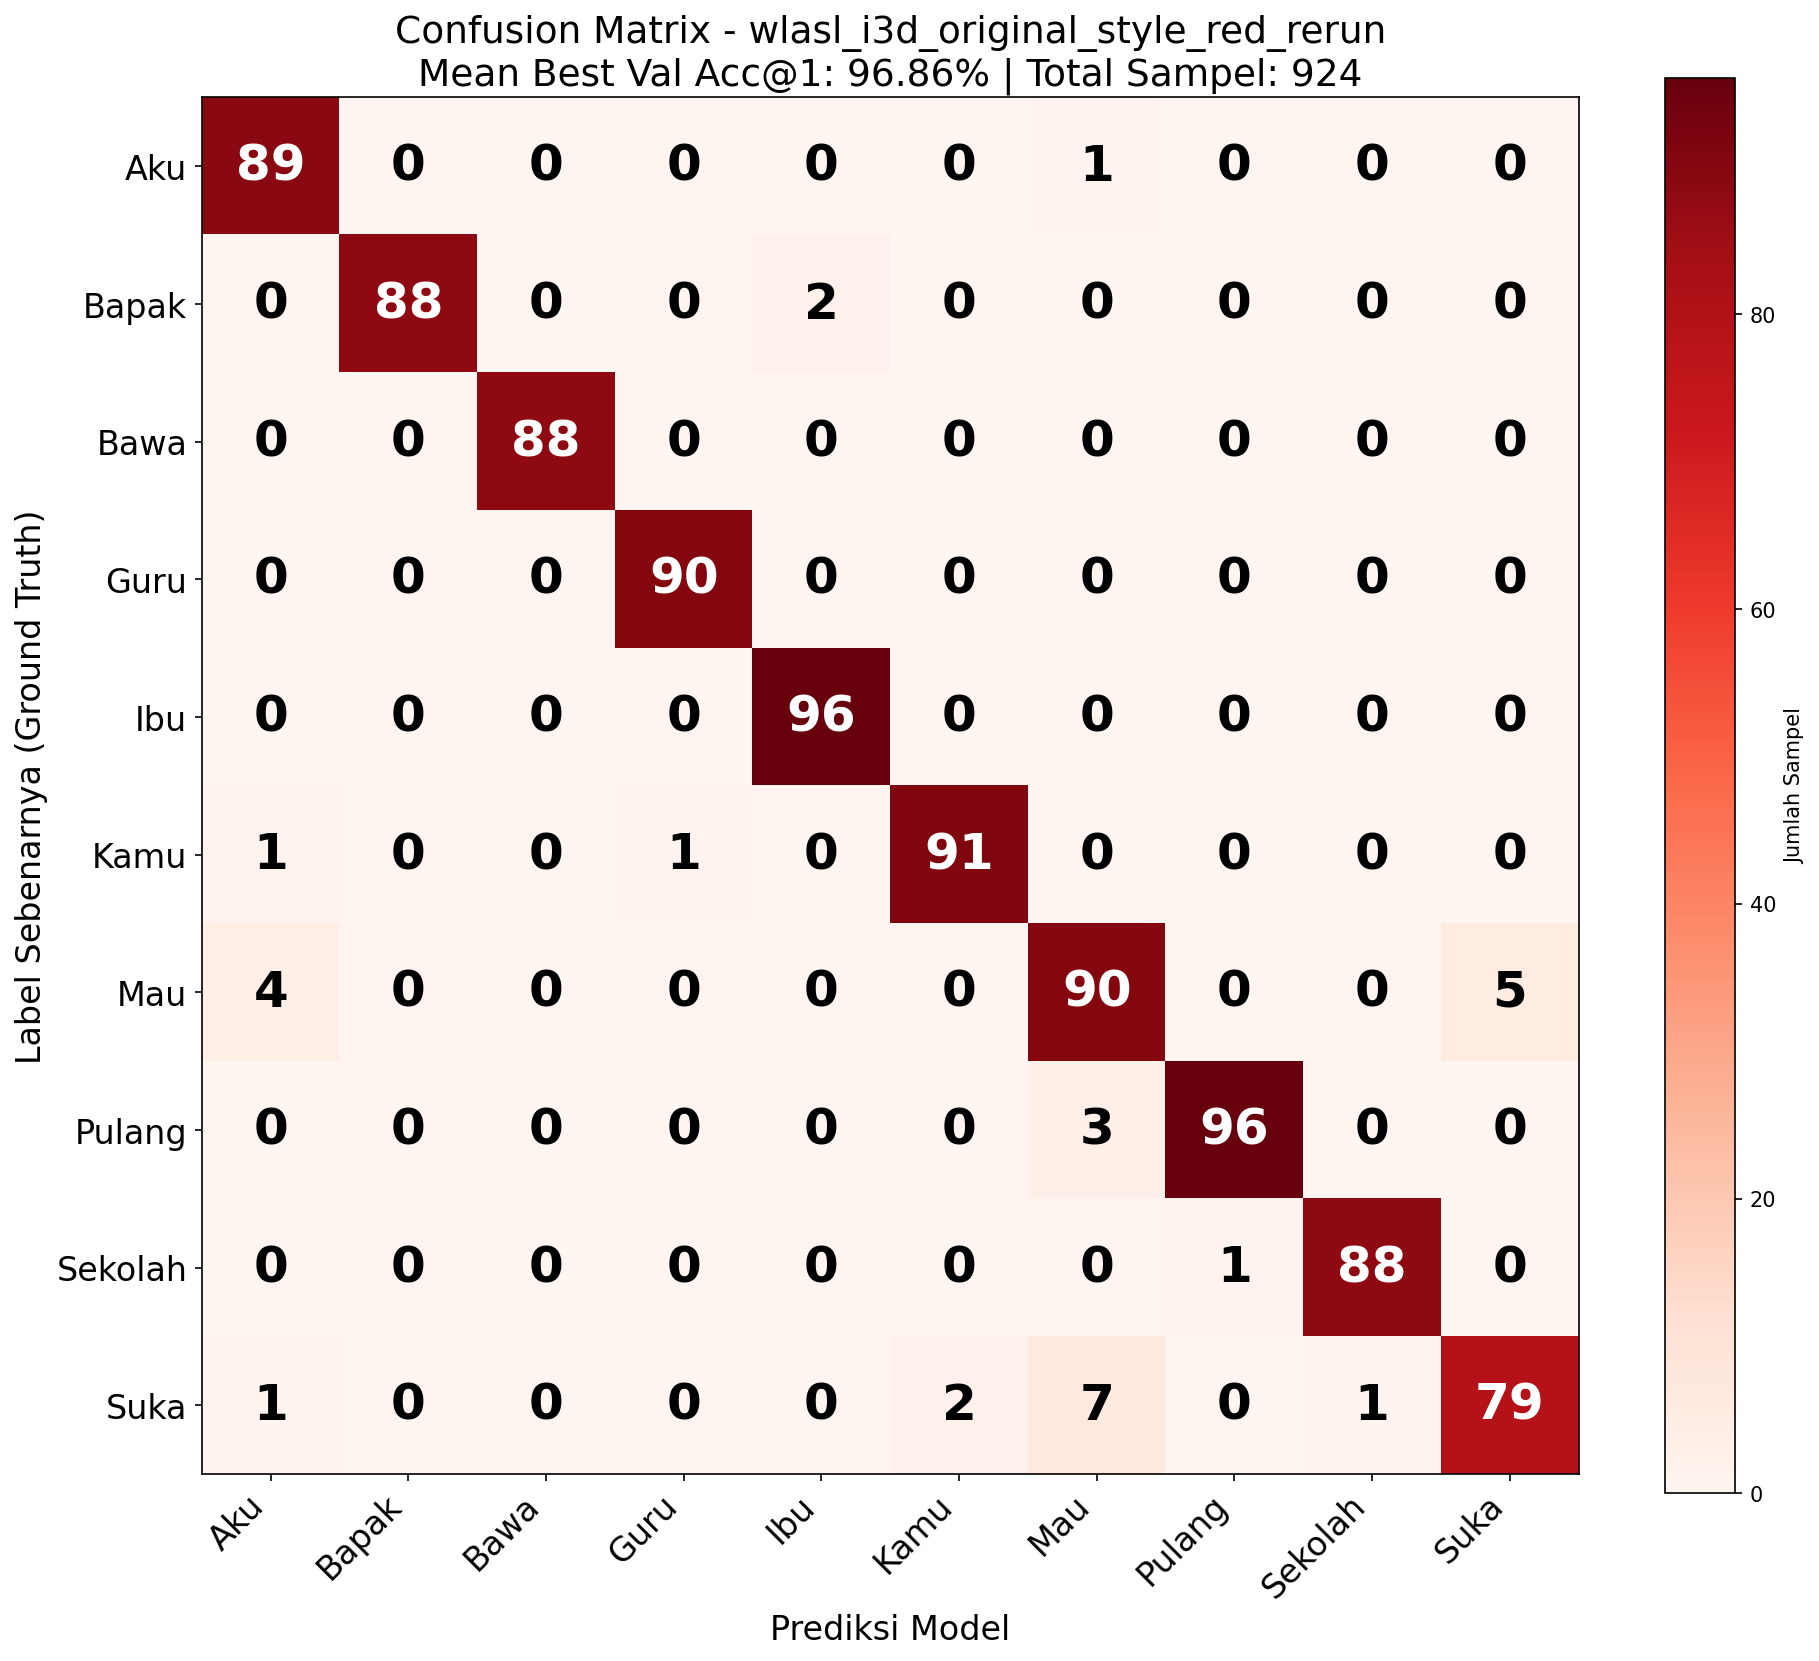
\includegraphics[width=0.95\textwidth]{figure/cm_i3d_new_font.png}
\caption{\textit{Confusion matrix} gabungan semua fold model I3D \textit{baseline}}
\label{fig:4.cm_i3d}
\end{figure}

\textit{Confusion matrix} I3D pada Gambar~\ref{fig:4.cm_i3d} menampilkan diagonal yang sangat dominan dengan intensitas tinggi di seluruh kelas, mencerminkan akurasi yang hampir sempurna. Sel-sel di luar diagonal hampir seluruhnya bernilai nol atau mendekati nol, menunjukkan bahwa kesalahan klasifikasi sangat jarang terjadi, pola yang sebanding dengan E12 namun lebih merata di seluruh kelas. Hal ini berbeda jauh dengan \textit{confusion matrix} VideoMAE E5 (Gambar~\ref{fig:4.cm_e5}) yang memperlihatkan distribusi kesalahan yang jauh lebih menyebar, khususnya pada kelas \textit{Suka}, \textit{Sekolah}, dan \textit{Pulang}.\par

Secara keseluruhan, E12 (VideoMAE ViT-Base + K400) tampil sebagai model terbaik dengan 97.18\%, diikuti I3D (96.86\%), ViViT (94.81\%), dan E11 (93.94\%). Keunggulan E12 dapat dikaitkan dengan dua faktor: (1) kapasitas ViT-Base yang lebih besar dibandingkan ViT-Small pada E11 memungkinkan representasi fitur yang lebih kaya, dan (2) domain K400 dengan \textit{dense sampling} mungkin lebih sesuai untuk menangkap fase gerak kritis dalam gestur SIBI. Selisih E12 atas I3D yang hanya 0.32 poin persentase menunjukkan bahwa VideoMAE yang dikonfigurasi dengan benar dapat bersaing dengan model CNN 3D yang secara historis unggul pada dataset kecil. ViViT menunjukkan performa yang kompetitif meski menggunakan arsitektur yang berbeda dari VideoMAE, mengindikasikan bahwa model \textit{Transformer} video yang di-\textit{fine-tune} dengan baik dari bobot K400 secara umum mampu mengklasifikasikan gestur SIBI dengan akurasi tinggi. Faktor yang paling menentukan bukan arsitektur atau ukuran model, melainkan kualitas bobot \textit{pre-train} dan strategi pelatihan yang tepat, terutama penonaktifan augmentasi yang terbukti kontraproduktif pada dataset bahasa isyarat SIBI.\par

Meskipun seluruh model mencapai akurasi tinggi, dua kelas yang secara konsisten menunjukkan F1-\textit{score} terendah di semua arsitektur adalah \textit{Suka} dan \textit{Mau}. Pada E12, \textit{Suka} memperoleh F1 0.91 dan \textit{Mau} memperoleh F1 0.90, keduanya paling rendah dibandingkan kelas lain meskipun masih tergolong tinggi secara absolut. Pola ini konsisten dengan temuan pada model sebelumnya: \textit{Suka} pada E9 mencapai F1 0.53 sementara mayoritas kelas sudah di atas 0.60, dan pada E5 nilai \textit{Mau} (F1 0.52) dan \textit{Suka} (F1 0.31) tertinggal jauh dari kelas lain. Analisis \textit{confusion matrix} memperlihatkan bahwa sebagian sampel \textit{Suka} cenderung terprediksi sebagai \textit{Mau}, dan sebaliknya, mengindikasikan kemiripan visual yang tinggi di antara keduanya. Secara linguistik, kedua gestur ini melibatkan gerakan tangan yang diarahkan ke area dada atau perut dengan orientasi telapak yang serupa, sehingga perbedaan antar keduanya bertumpu pada detail halus seperti lintasan akhir tangan dan kecepatan gerak. Di samping itu, kedua kelas ini menunjukkan variasi gaya isyarat antar-penutur yang lebih tinggi dibandingkan kelas seperti \textit{Bawa} atau \textit{Guru} yang memiliki bentuk tangan lebih distinktif. Kombinasi kemiripan visual antar kelas dan variasi antar-penutur yang besar menjadikan \textit{Mau} dan \textit{Suka} sebagai pasangan kelas yang paling menantang, dan perbaikan lebih lanjut pada kedua kelas ini kemungkinan memerlukan penambahan data atau augmentasi berbasis pose tangan yang lebih spesifik.\par
Meskipun seluruh model mencapai akurasi tinggi, dua kelas yang secara konsisten menunjukkan F1-\textit{score} terendah di semua arsitektur adalah \textit{Suka} dan \textit{Mau}. Pada E12, \textit{Suka} memperoleh F1 0.91 dan \textit{Mau} memperoleh F1 0.90, keduanya paling rendah dibandingkan kelas lain meskipun masih tergolong tinggi secara absolut. Pola ini konsisten dengan temuan pada model sebelumnya: \textit{Suka} pada E9 mencapai F1 0.53 sementara mayoritas kelas sudah di atas 0.60, dan pada E5 nilai \textit{Mau} (F1 0.52) dan \textit{Suka} (F1 0.31) tertinggal jauh dari kelas lain. Analisis \textit{confusion matrix} memperlihatkan bahwa sebagian sampel \textit{Suka} cenderung terprediksi sebagai \textit{Mau}, dan sebaliknya, mengindikasikan kemiripan visual yang tinggi di antara keduanya. Secara linguistik, kedua gestur ini melibatkan gerakan tangan yang diarahkan ke area dada atau perut dengan orientasi telapak yang serupa, sehingga perbedaan antar keduanya bertumpu pada detail halus seperti lintasan akhir tangan dan kecepatan gerak. Di samping itu, kedua kelas ini menunjukkan variasi gaya isyarat antarpenutur yang lebih tinggi dibandingkan kelas seperti \textit{Bawa} atau \textit{Guru} yang memiliki bentuk tangan lebih distinktif. Kombinasi kemiripan visual antarkelas dan variasi antarpenutur yang besar menjadikan \textit{Mau} dan \textit{Suka} sebagai pasangan kelas yang paling menantang, dan perbaikan lebih lanjut pada kedua kelas ini kemungkinan memerlukan penambahan data atau augmentasi berbasis pose tangan yang lebih spesifik.\par


%===========================================================================
%===========================================================================
\subsection{Analisis Waktu Inferensi Model} \label{IV.Inferensi}
%===========================================================================

Selain akurasi klasifikasi, waktu inferensi merupakan faktor penting dalam menilai kelayakan \textit{deployment} model pada aplikasi nyata. Pengukuran dilakukan menggunakan video asli dari dataset (5 video dipilih secara acak) pada GPU NVIDIA GeForce RTX 3050 Laptop (4\,GB VRAM, CUDA 12.4). Setiap video terlebih dahulu melalui tahap pra-pemrosesan lengkap yang identik dengan pipeline pelatihan masing-masing model, meliputi dekode video, \textit{sampling} frame, \textit{resize}, dan normalisasi, dan hasilnya disimpan sebagai tensor di GPU sebelum pengukuran dimulai. Dengan cara ini, waktu yang dicatat hanya mencerminkan waktu inferensi model tanpa dipengaruhi variasi latensi I/O atau \textit{decoding} video antar-iterasi. Sinkronisasi CUDA (\texttt{torch.cuda.synchronize()}) diterapkan sebelum dan sesudah setiap inferensi untuk memastikan akurasi pengukuran pada GPU. Setiap model diukur pada kelima \textit{best checkpoint} masing-masing fold dengan 10 iterasi \textit{warm-up} dan 50 pengulangan, kemudian dirata-ratakan lintas fold.\par
Selain akurasi klasifikasi, waktu inferensi merupakan faktor penting dalam menilai kelayakan \textit{deployment} model pada aplikasi nyata. Pengukuran dilakukan menggunakan video asli dari dataset (5 video dipilih secara acak) pada GPU NVIDIA GeForce RTX 3050 Laptop (4\,GB VRAM, CUDA 12.4). Setiap video terlebih dahulu melalui tahap prapemrosesan lengkap yang identik dengan pipeline pelatihan masing-masing model, meliputi dekode video, \textit{sampling} frame, \textit{resize}, dan normalisasi, dan hasilnya disimpan sebagai tensor di GPU sebelum pengukuran dimulai. Dengan cara ini, waktu yang dicatat hanya mencerminkan waktu inferensi model tanpa dipengaruhi variasi latensi I/O atau \textit{decoding} video antariterasi. Sinkronisasi CUDA (\texttt{torch.cuda.synchronize()}) diterapkan sebelum dan sesudah setiap inferensi untuk memastikan akurasi pengukuran pada GPU. Setiap model diukur pada kelima \textit{best checkpoint} masing-masing fold dengan 10 iterasi \textit{warm-up} dan 50 pengulangan, kemudian dirata-ratakan lintas fold.\par

Setiap model memiliki pipeline prapemrosesan yang berbeda sesuai protokol pelatihannya; perbedaan tersebut dirangkum pada Tabel~\ref{tab:4.preproc_bench}.

\begin{table}[H]
\centering
\caption{Konfigurasi prapemrosesan tiap model pada eksperimen inferensi}
\label{tab:4.preproc_bench}
\footnotesize
\begin{tabular}{|l|l|r|l|}
\hline
\rowcolor{gray!15} \multicolumn{1}{|c|}{\textbf{Model}} & \multicolumn{1}{c|}{\makecell[c]{\textbf{Library}\\\textbf{Dekode Video}}} & \multicolumn{1}{c|}{\textbf{Frame}} & \multicolumn{1}{c|}{\textbf{Normalisasi}} \\
\hline
VideoMAE ViT-Small + SSV2 & decord & 16 & ImageNet ($\mu/\sigma$) \\
\hline
VideoMAE ViT-Base + K400  & decord & 16 & ImageNet ($\mu/\sigma$) \\
\hline
ViViT-B/16x2              & decord & 32 & $(x-0.5)/0.5$ \\
\hline
I3D RGB                   & OpenCV & 64 & $(x/255)\times2-1$ \\
\hline
\end{tabular}
\end{table}

Kode~\ref{lst:benchmark_fn} menunjukkan fungsi pengukuran yang dipakai secara identik untuk seluruh arsitektur.

\begin{lstlisting}[caption={Kode pengukuran waktu inferensi model (dipakai untuk semua arsitektur)}, label={lst:benchmark_fn}]
def benchmark(model, video_paths, device, warmup=10, runs=50):
    # Pra-pemrosesan dilakukan SEKALI di luar timer
    # Prapemrosesan dilakukan SEKALI di luar timer
    tensors = [preprocess_video(p).to(device) for p in video_paths]

    with torch.no_grad():
        # Warm-up: memastikan GPU dalam kondisi stabil
        for i in range(warmup):
            model(tensors[i % len(tensors)])
            if device.type == "cuda":
                torch.cuda.synchronize()

        # Pengukuran: hanya waktu inferensi yang dicatat
        times = []
        for i in range(runs):
            x = tensors[i % len(tensors)]
            if device.type == "cuda":
                torch.cuda.synchronize()   # pastikan GPU idle sebelum mulai
            t0 = time.perf_counter()
            model(x)
            if device.type == "cuda":
                torch.cuda.synchronize()   # tunggu GPU selesai
            times.append((time.perf_counter() - t0) * 1000)  # ms

    return {"mean": statistics.mean(times), "std": statistics.stdev(times),
            "min": min(times), "max": max(times),
            "median": statistics.median(times)}
\end{lstlisting}

Tabel~\ref{tab:4.inferensi} merangkum rata-rata waktu inferensi tiap model.

\begin{table}[H]
\centering
\caption{Rata-rata waktu inferensi model pada GPU RTX 3050 Laptop}
\label{tab:4.inferensi}
\footnotesize
\begin{tabular}{|l|r|r|r|}
\hline
\rowcolor{gray!15} \multicolumn{1}{|c|}{\textbf{Model}} & \multicolumn{1}{c|}{\textbf{Param.}} & \multicolumn{1}{c|}{\makecell[c]{\textbf{Frame}\\\textbf{Input}}} & \multicolumn{1}{c|}{\makecell[c]{\textbf{Rata-rata}\\\textbf{(ms)}}} \\
\hline
VideoMAE ViT-Small + SSV2 (E11/E5) & 21.9\,jt &  16 &  66.36 \\
\hline
I3D RGB                             & 12.3\,jt &  64 &  89.15 \\
\hline
VideoMAE ViT-Base + K400 (E12)      & 86.2\,jt &  16 & 168.83 \\
\hline
ViViT-B/16x2                        & 88.7\,jt &  32 & 467.09 \\
\hline
\end{tabular}
\end{table}

Hasil pada Tabel~\ref{tab:4.inferensi} menunjukkan bahwa jumlah parameter bukan satu-satunya penentu waktu inferensi; arsitektur komputasi dan jumlah frame yang diproses memainkan peran yang sama pentingnya.\par

Bukti pertama tampak pada perbandingan antara I3D dan VideoMAE ViT-Small. I3D hanya memiliki 12.3 juta parameter, lebih sedikit dari ViT-Small (21.9 juta), namun waktu inferensinya lebih lambat (89.15\,ms vs 66.36\,ms). Penyebabnya adalah jumlah frame: I3D memproses 64 frame sekaligus menggunakan konvolusi 3D yang harus melintasi seluruh dimensi temporal pada setiap blok \textit{Inception}-nya. Meskipun konvolusi 3D secara teoritis lebih ringan dari mekanisme \textit{attention}, beban akumulasi dari 64 frame menjadikan I3D lebih lambat dibandingkan ViT-Small yang hanya memproses 16 frame. Ini membuktikan bahwa semakin banyak frame yang diproses, semakin tinggi biaya komputasi, terlepas dari jumlah parameter model.\par

Bukti kedua dan paling kuat terlihat pada perbandingan ViViT dan VideoMAE ViT-Base. Keduanya memiliki jumlah parameter yang hampir identik, ViViT 88.7 juta dan ViT-Base 86.2 juta, namun waktu inferensi ViViT (467.09\,ms) hampir 2.8$\times$ lebih lambat dibandingkan ViT-Base (168.83\,ms). Perbedaan ini tidak dapat dijelaskan oleh parameter, melainkan oleh dua faktor: (1) ViViT memproses 32 frame sementara ViT-Base hanya 16 frame, dan (2) ViViT menggunakan \textit{full spatio-temporal self-attention} yang kompleksitasnya tumbuh kuadratik $\mathcal{O}(n^2)$ terhadap jumlah token video. Semakin banyak frame, semakin besar matriks \textit{attention} yang harus dihitung, sehingga latensi meningkat secara dramatis. Sebaliknya, VideoMAE ViT-Base menggunakan \textit{tubelet embedding} yang memadatkan informasi temporal sebelum masuk ke blok \textit{attention}, sehingga jumlah token yang diproses jauh lebih sedikit.\par

Satu-satunya kasus di mana parameter menjadi penentu utama adalah perbandingan antara ViT-Small dan ViT-Base, karena keduanya menggunakan arsitektur yang identik (VideoMAE, patch 16$\times$16, 16 frame, \textit{tubelet} 2). Dengan parameter ViT-Base $\approx$4$\times$ lebih banyak, waktu inferensinya meningkat $\approx$2.5$\times$, hubungan yang mendekati proporsional dan wajar untuk arsitektur sejenis.\par

Secara keseluruhan, seluruh model mampu menyelesaikan inferensi di bawah 470\,ms pada GPU kelas menengah, yang mengindikasikan kelayakan \textit{deployment} untuk aplikasi pengenalan bahasa isyarat berbasis video secara \textit{near real-time}. Dari eksperimen ini dapat disimpulkan bahwa pilihan jumlah frame dan strategi \textit{attention} jauh lebih menentukan latensi inferensi dibandingkan sekadar memperbandingkan jumlah parameter antar model.\par


%===========================================================================
\subsection{Rangkuman Hasil Seluruh Eksperimen} \label{IV.Rangkuman}
%===========================================================================

Tabel~\ref{tab:4.rangkuman} merangkum hasil terbaik dari seluruh eksperimen untuk memberikan gambaran perjalanan peningkatan performa secara menyeluruh.\par

\begin{table}[H]
\centering
\caption{Rangkuman hasil terbaik dari seluruh eksperimen VideoMAE, ViViT, dan I3D}
\label{tab:4.rangkuman}
{\setlength{\tabcolsep}{3pt}%
\footnotesize
\begin{tabularx}{\linewidth}{|l|>{\raggedright\arraybackslash}p{2.5cm}|>{\raggedright\arraybackslash}X|>{\raggedleft\arraybackslash}p{2.3cm}|>{\raggedleft\arraybackslash}p{1.3cm}|}
\hline
\rowcolor{gray!15} \multicolumn{1}{|c|}{\textbf{Kode}} & \multicolumn{1}{>{\centering\arraybackslash}p{2.5cm}|}{\makecell[c]{\textbf{Kelompok}\\\textbf{Eksperimen}}} & \multicolumn{1}{>{\centering\arraybackslash}X|}{\textbf{Konfigurasi}} & \multicolumn{1}{>{\centering\arraybackslash}p{2.3cm}|}{\makecell[c]{\textbf{Rerata} $\pm$ \textbf{Std}\\\textbf{(\%)}}} & \multicolumn{1}{c|}{\makecell[c]{\textbf{Acc@1}\\\textbf{(\%)}}} \\
\hline
E3   & \textit{Backbone} \& \textit{Pre-train}       & ViT-Small + SSV2 (\textit{fine-tune})                  & $35.18 \pm 4.32$ & 42.39 \\
\hline
E5   & Strategi Pelatihan                             & \textit{Two-Stage Pre-train} (50 ep, \textit{uniform}) & $63.85 \pm 3.70$ & 70.27 \\
\hline
E9   & Jumlah \textit{Epoch}                          & \textit{Two-Stage Pre-train} (100 ep)                  & $66.56 \pm 2.49$ & 70.81 \\
\hline
E11  & Pengaruh Augmentasi                            & ViT-Small + SSV2, tanpa \textit{mixup/CutMix/reprob}   & $93.94 \pm 1.29$ & 95.68 \\
\hline
E12  & \makecell[l]{Perbandingan\\Lintas Arsitektur}  & ViT-Base + K400, \textit{dense}, tanpa augmentasi      & $97.18 \pm 1.51$ & 98.92 \\
\hline
ViViT & \makecell[l]{Perbandingan\\Lintas Arsitektur} & ViViT-B/16x2 + K400, 32 frame                          & $94.81 \pm 1.69$ & 96.20 \\
\hline
I3D  & \makecell[l]{Perbandingan\\Lintas Arsitektur}  & I3D + ImageNet (\textit{fine-tune})                    & $96.86 \pm 1.04$ & 98.38 \\
\hline
\end{tabularx}}
\end{table}

Tabel~\ref{tab:4.rangkuman} memperlihatkan perjalanan peningkatan performa yang bertahap melalui seluruh kelompok eksperimen. Lompatan terbesar pertama terjadi dari E3 ke E5 (35.18\% $\rightarrow$ 63.85\%), peningkatan sebesar 28.67 poin persentase yang semata-mata berasal dari penerapan strategi \textit{two-stage pre-train} dengan bobot SSV2. Perlu dicatat bahwa E5 sekaligus merepresentasikan konfigurasi terbaik dari dua kelompok eksperimen lainnya: konfigurasi \textit{uniform sampling} pada analisis strategi \textit{sampling} (Bagian~\ref{IV.Sek3}) dan konfigurasi 50 epoch pada analisis jumlah epoch (Bagian~\ref{IV.Sek4}), sehingga tidak dicantumkan terpisah di tabel rangkuman. Peningkatan berikutnya lebih moderat: penambahan epoch dari 50 ke 100 pada E9 menghasilkan kenaikan 2.71 poin (66.56\%), sementara perbedaan strategi \textit{sampling} antara E10 dan E5 memberikan selisih 7.78 poin persentase. Lompatan terbesar kedua terjadi dari E5 ke E11 (63.85\% $\rightarrow$ 93.94\%) ketika augmentasi \textit{mixup}, \textit{CutMix}, dan \textit{reprob} dinonaktifkan, peningkatan 30.09 poin persentase yang mengungkap bahwa ketiga teknik tersebut merusak konteks gerakan detail yang menjadi pembeda utama antar isyarat SIBI. Pada perbandingan lintas arsitektur, E12 (97.18\%) tampil sebagai model terbaik, diikuti I3D (96.86\%), ViViT (94.81\%), dan E11 (93.94\%). Secara keseluruhan, seluruh kelompok eksperimen mengidentifikasi enam faktor kunci secara berurutan berdasarkan besarnya pengaruh terhadap performa: (1) ketersediaan bobot \textit{pre-train} yang relevan, (2) menjaga keutuhan konteks gerakan dengan tidak menerapkan augmentasi yang merusak sekuens spasio-temporal, (3) strategi pelatihan dua tahap yang efektif, (4) pemilihan arsitektur dan ukuran \textit{backbone}, (5) strategi \textit{sampling} yang mencakup keseluruhan temporal gestur, dan (6) durasi pelatihan yang memadai.\par


\section{Analisis Kesalahan} \label{IV.AnalisisKesalahan}
%===========================================================================

Bagian ini menyajikan analisis mendalam terhadap pola kesalahan klasifikasi yang masih terjadi meskipun model telah mencapai performa optimalnya. Analisis ini bertujuan untuk memahami karakteristik spesifik dari sampel-sampel yang gagal diprediksi dengan benar, sehingga dapat memberikan wawasan mengenai batasan kemampuan arsitektur model serta kompleksitas visual dan temporal dari kelas-kelas tertentu dalam dataset SIBI. Melalui telaah \textit{confusion matrix} dan observasi kualitatif terhadap frame video, evaluasi difokuskan untuk mengidentifikasi kelas-kelas yang secara persisten menjadi sumber \textit{misclassification} utama.\par

Meskipun seluruh model mencapai akurasi tinggi, dua kelas yang secara konsisten menunjukkan F1-\textit{score} terendah di semua arsitektur adalah Suka dan Mau. Pada E12, Suka memperoleh F1 0.91 dan Mau memperoleh F1 0.90, keduanya paling rendah dibandingkan kelas lain meskipun masih tergolong tinggi secara absolut. Pola ini konsisten dengan temuan pada model sebelumnya: Suka pada E9 mencapai F1 0.53 sementara mayoritas kelas sudah di atas 0.60, dan pada E5 nilai Mau (F1 0.52) dan Suka (F1 0.31) tertinggal jauh dari kelas lain. Analisis \textit{confusion matrix} memperlihatkan bahwa sebagian sampel Suka cenderung terprediksi sebagai Mau, dan sebaliknya, sehingga pasangan ini merupakan sumber \textit{misclassification} yang paling persisten bahkan setelah performa model secara umum sudah sangat tinggi.\par

Secara visual, kemiripan tersebut dapat dipahami dari contoh frame representatif: baik Mau maupun Suka sama-sama menempatkan tangan dominan pada area artikulasi tengah, yakni sekitar dada hingga perut, dengan tubuh menghadap kamera dan latar yang seragam. Pada level citra tunggal, keduanya tidak memiliki pembeda kasar yang setajam kelas seperti Bawa atau Guru. Hal ini penting karena menunjukkan bahwa satu frame statis saja sering belum cukup untuk membedakan kedua kata tersebut; sinyal pembeda utama justru terletak pada bagaimana tangan bergerak dari posisi awal menuju posisi akhir. Gambar~\ref{fig:4.mau_vs_suka} menunjukkan perbandingan visual sampel gerakan dari kelas Mau dan Suka.\par

\begin{figure}[H]
\centering
\makebox[\textwidth][c]{\fbox{\begin{minipage}{1.1\textwidth}
\centering
% Row 1: Mau
\begin{subfigure}[b]{0.24\linewidth}
  \centering
  
\includegraphics[width=\linewidth]{figure/sampel_blurred/Mau_099_sample1.png}
  \caption{Mau (Sampel 1)}
\end{subfigure}
\hfill
\begin{subfigure}[b]{0.24\linewidth}
  \centering
  
\includegraphics[width=\linewidth]{figure/sampel_blurred/Mau_099_sample2.png}
  \caption{Mau (Sampel 2)}
\end{subfigure}
\hfill
\begin{subfigure}[b]{0.24\linewidth}
  \centering
  
\includegraphics[width=\linewidth]{figure/sampel_blurred/Mau_099_sample3.png}
  \caption{Mau (Sampel 3)}
\end{subfigure}
\hfill
\begin{subfigure}[b]{0.24\linewidth}
  \centering
  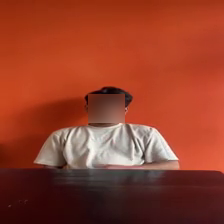
\includegraphics[width=\linewidth]{figure/sampel_blurred/Mau_099_sample4.png}
  \caption{Mau (Sampel 4)}
\end{subfigure}
\vspace{0.5cm}

% Row 2: Suka
\begin{subfigure}[b]{0.24\linewidth}
  \centering
  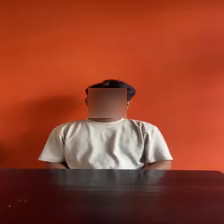
\includegraphics[width=\linewidth]{figure/sampel_blurred/Suka_090_sample1.png}
  \caption{Suka (Sampel 1)}
\end{subfigure}
\hfill
\begin{subfigure}[b]{0.24\linewidth}
  \centering
  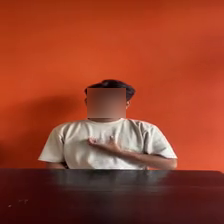
\includegraphics[width=\linewidth]{figure/sampel_blurred/Suka_090_sample2.png}
  \caption{Suka (Sampel 2)}
\end{subfigure}
\hfill
\begin{subfigure}[b]{0.24\linewidth}
  \centering
  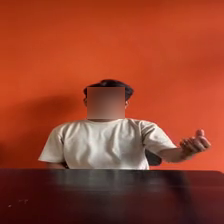
\includegraphics[width=\linewidth]{figure/sampel_blurred/Suka_090_sample3.png}
  \caption{Suka (Sampel 3)}
\end{subfigure}
\hfill
\begin{subfigure}[b]{0.24\linewidth}
  \centering
  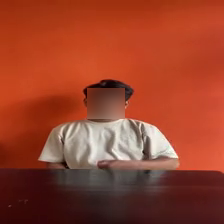
\includegraphics[width=\linewidth]{figure/sampel_blurred/Suka_090_sample4.png}
  \caption{Suka (Sampel 4)}
\end{subfigure}
\end{minipage}}}
\captionsetup{justification=raggedright,singlelinecheck=false}
\caption{Perbandingan visual sampel gerakan gestur Mau (baris atas) dan Suka (baris bawah)}
\label{fig:4.mau_vs_suka}
\end{figure}

Kondisi ini menegaskan bahwa untuk bahasa isyarat, model tidak bisa hanya mengandalkan fitur spasial tunggal. Kemampuan model untuk menangkap \textit{temporal dynamics}---perubahan antar-frame---menjadi sangat krusial. Pada kelas Mau dan Suka, model sering kali 'bingung' karena keduanya memiliki fitur spasial yang identik pada frame-frame tertentu, dan hanya dibedakan oleh kecepatan atau arah pergerakan yang sangat halus. Ini adalah tantangan utama dalam \textit{fine-grained action recognition}, di mana kelas-kelas tertentu memerlukan \textit{temporal receptive field} yang lebih panjang atau mekanisme \textit{attention} yang lebih sensitif terhadap perubahan kecil di sepanjang waktu. Kesalahan yang terjadi pada kelas ini sebagian besar adalah masalah dinamika gestur daripada masalah bentuk pose tunggal.\par

Secara temporal, kedua gestur sama-sama memuat lintasan tangan pendek di ruang artikulasi yang berdekatan, sehingga perbedaannya bertumpu pada detail mikro seperti arah lintasan akhir, besar amplitudo gerak, perubahan orientasi telapak, dan \textit{timing} saat tangan berhenti. Jika model gagal menangkap salah satu fase tersebut, maka representasi kedua kelas menjadi sangat berdekatan di ruang fitur. Gejala ini terlihat jelas pada E10, di mana \textit{dense sampling} menurunkan F1 kelas Suka hingga 0.14 dan banyak sampelnya diprediksi sebagai Mau atau Kamu; hal ini mengindikasikan bahwa ketika cakupan temporal tidak lengkap, petunjuk pembeda pada fase awal atau akhir gestur mudah hilang. Sebaliknya, pada E12, ViViT, dan I3D, kesalahan tinggal tersisa dalam jumlah kecil, tetapi tetap terkonsentrasi pada dua kelas ini, yang menunjukkan bahwa bahkan model dengan representasi spasio-temporal kuat masih harus bekerja lebih keras untuk membedakan pola gerak yang sangat mirip secara lokal.\par

Dari sudut pandang linguistik bahasa isyarat, temuan ini memperlihatkan bahwa Mau dan Suka berbagi parameter manual tingkat tinggi yang serupa, tetapi dibedakan oleh konfigurasi sub-gerak yang lebih halus. Karena itu, kesalahan klasifikasi keduanya bukan sekadar akibat kekurangan data, melainkan mencerminkan batas diskriminasi model terhadap isyarat yang memiliki kemiripan lokasi artikulasi dan orientasi awal. Analisis ini memberi bobot ilmiah tambahan pada hasil penelitian: untuk tugas pengenalan SIBI berbasis video, evaluasi tidak cukup berhenti pada akurasi global, tetapi perlu menelaah pasangan kelas yang secara linguistik dan visual berdekatan. Perbaikan lebih lanjut pada pasangan Mau--Suka kemungkinan memerlukan penambahan sampel dengan variasi lintasan gerak yang lebih kaya, resolusi temporal yang lebih padat namun tetap mencakup keseluruhan gestur, atau pendekatan yang lebih eksplisit memodelkan pose tangan dan perubahan orientasi antar-frame.\par


%===========================================================================
